\documentclass[12pt]{article}
\usepackage[english]{babel}
\usepackage{amsmath}
\usepackage{graphicx}
\usepackage{enumerate}
\usepackage{caption}
\usepackage{booktabs}
\usepackage{natbib}
\usepackage{subcaption}
\usepackage{amssymb}
\usepackage[colorinlistoftodos]{todonotes}
\usepackage{multicol}
\usepackage{authblk}
\usepackage{url}
\usepackage{color}
\newcommand{\comment}[1]{{\color{blue} #1}}
\newcommand{\brittany}[1]{{\color{cyan} Brittany says: #1}}
\newcommand{\mike}[1]{{\color{orange} #1}}
% ... for graphics
\graphicspath{{./}{figs/}}
% ... for easy and consistent referencing
\newcommand{\figref}[1]{Figure~\ref{#1}}
% ... mathematical symbols
\def\R{{\mathbb R}}

%\pdfminorversion=4
% NOTE: To produce blinded version, replace "0" with "1" below.
\newcommand{\blind}{0}

% DON'T change margins - should be 1 inch all around.
\addtolength{\oddsidemargin}{-.5in}%
\addtolength{\evensidemargin}{-.5in}%
\addtolength{\textwidth}{1in}%
\addtolength{\textheight}{1.3in}%
\addtolength{\topmargin}{-.8in}%


\begin{document}

%\bibliographystyle{natbib}

\def\spacingset#1{\renewcommand{\baselinestretch}%
{#1}\small\normalsize} \spacingset{1}


%%%%%%%%%%%%%%%%%%%%%%%%%%%%%%%%%%%%%%%%%%%%%%%%%%%%%%%%%%%%%%%%%%%%%%%%%%%%%%

\if0\blind
{
  \title{\bf Topological Hypothesis Tests for the Large-Scale Structure of the Universe}
  \author{Mike Wu\\
    Department of Computer Science, Yale University \\
    Jessi Cisewski\thanks{
    Corresponding author.  The authors gratefully acknowledge Yale Information Technology Services}\hspace{.2cm} \\
    Department of Statistics, Yale University \\
    Brittany T. Fasy\\
School of Computing, Montana State University \\
    Wojciech Hellwing \\
    Institute of Cosmology and Gravitation, University of Portsmouth \\
    Mark R. Lovell\\
    Gravitation AstroParticle Physics, University of Amsterdam \\
    Alessandro Rinaldo\\
    Department of Statistics, Carnegie Mellon University \\
    Larry Wasserman\\
    Department of Statistics, Carnegie Mellon University \\
  }
  \maketitle
} \fi

\if1\blind
{
  \bigskip
  \begin{center}
    {\LARGE\bf Title}
\end{center}
  \medskip
} \fi

%%%%%%%%%%%%%%%%%%%%%%%%%%%%%%%%%%%%%%%%%%%%%%%%%%%%%%%
%% SECTION: ABSTRACT
%%%%%%%%%%%%%%%%%%%%%%%%%%%%%%%%%%%%%%%%%%%%%%%%%%%%%%%

\bigskip
\begin{abstract}
The large-scale structure (LSS) of the Universe is an intricate and spatially complex web. In order to understand the physics of the Universe, theoretical and computational cosmologists develop large-scale simulations that allow for visualizing and analyzing the LSS under varying physical assumptions. In particular, different realizations of dark matter, warm and cold, are thought to lead to contrasting velocities of cosmic structure formation. However, rigorous comparisons and inference on such complicated structures can be problematic.  We present a framework for hypothesis testing of LSS using persistent homology. The randomness in the data (due to measurement error or topological noise) is transferred to randomness in the topological summaries, which provides an infrastructure for inference. These tests allow for statistical comparisons between complicated spatial data such as LSS in cosmology, but are also relevant to other areas of science. We present several test statistics using persistence diagrams, carry-out a simulation study to investigate the suitableness of the proposed test statistics, and finally apply the inference framework to study topological disparities between assumptions of warm and cold dark matter.
\end{abstract}

\noindent%
{\it Keywords:} Astrostatistics, persistent homology, topological data analysis 

%%%%%%%%%%%%%%%%%%%%%%%%%%%%%%%%%%%%%%%%%%%%%%%%%%%%%%%
%% SECTION: INTRODUCTION
%%%%%%%%%%%%%%%%%%%%%%%%%%%%%%%%%%%%%%%%%%%%%%%%%%%%%%%

\spacingset{1.45} % DON'T change the spacing!
\section{Introduction}
\label{sec:intro}

{\color{blue} Real observations of cosmic web:  Great Wall \citep{geller1989mapping}, Sloan Great Wall \citep{gott2005map}, gas \citep{cantalupo2014cosmic}.}

Rigorous comparisons of spatially complex web-like data such as the large-scale structure (LSS) of the Universe (see \figref{fig:introData}) are notoriously challenging due, in part, to the difficulty in capturing the randomness of geometric and topological structures.  However, these comparisons are important because there exists information about cosmological parameters in the structure. We propose a framework for constructing topological hypothesis tests using ideas from an emerging area of topological data analysis (TDA) called persistent homology. Persistent homology offers a novel way to represent, visualize, and interpret complex data by extracting topological features, which can be used to infer properties of the underlying structures, as seen in astronomy \citep{Sousbie2011, SousbieEtAl2011, van2011alpha,cisewski2014non} among other areas of science \citep{bendich2014persistent, duong2012closed}.

The large-scale structure (LSS) of the Universe is an important example of a spatially complex structure, and is fittingly referred to as the \emph{Cosmic Web} \citep{bond1996filaments,springel2006large}. The LSS of the Universe is a focus of manifold scientific research because its properties reveal information about the underlying physics and formation of our Universe \citep{davis1985evolution}.  For example, LSS can reveal characteristics of dark energy, which is thought to be the driver of the acceleration of the Universe \citep{Sanchez:2012aa}.  In order to study theoretical aspects of the formation and evolution of LSS, cosmologists develop large simulations and can adjust the physical inputs and evaluate their effects on the LSS \citep{cooray2002halo,centrella1983three,doroshkevich1980two,schaye2015eagle}. One such input is related to the nature of dark matter (DM). The received theory is that the Universe is made up of dark energy, DM, and baryonic matter. However, the nature of DM is still a mystery, but there are hypotheses regarding its possible particle behavior. Hot DM would consist of particles that travel with ultrarelativistic speeds, while cold DM particles would move much slower. For an easy introduction to DM, see \cite[p. 61-63]{HilbeEtAl2014}.

Though the generally accepted and best supported cosmological model assumes \emph{cold dark matter} (known as $\Lambda$CDM), there are some elements of disagreement with observations \citep{SchneiderEtAl2012}. Furthermore, it has been demonstrated through cosmological simulations that the nature of DM affects the development and formation of LSS \citep{SchneiderEtAl2012}.
In \figref{fig:introData}, one realization of our Universe under CDM from the EAGLE cosmological simulation \citep{schaye2015eagle} is displayed, along with a realization assuming WDM. Though there are similarities in shape of the densest regions (called \emph{filaments}), there are differences in the distribution of matter about these filaments.

\begin{figure}[htp!]
  \centering
  \begin{subfigure}{.40\textwidth}
    \centering
    \caption{WDM Simulation}  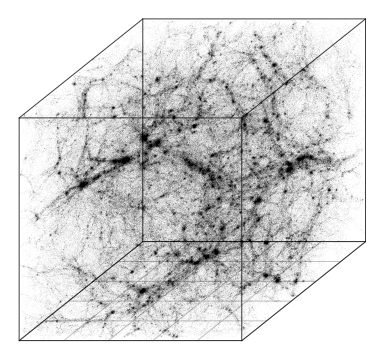
\includegraphics[width=\linewidth]{figure_1_whole_wdm.png}
    \label{fig:introDataWDM}
  \end{subfigure}
    \begin{subfigure}{.40\textwidth}
    \centering
    \caption{CDM Simulation}  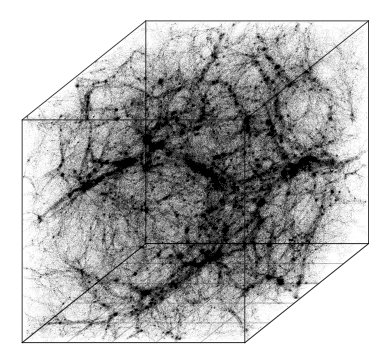
\includegraphics[width=\linewidth]{figure_1_whole_cdm.png}
    \label{fig:introDataCDM}
  \end{subfigure}
    \caption{Dark matter-only cosmological simulations assuming (a) warm dark matter (WDM) and (b) cold dark matter (CDM).  See Section~\ref{sec:application} for details. }
    \label{fig:introData}
\end{figure}

In this paper, we wish to better identify differences in the topology between structures using persistent homology. We begin with an introduction to persistent homology followed by the proposed hypothesis testing framework. Then we carry out a simulation study to investigate the performance of the proposed statistics followed by more background on LSS. And finally, we apply the hypothesis tests to quantify the topological disparities between warm and cold DM using cosmological simulation data. We end with concluding remarks.


%%%%%%%%%%%%%%%%%%%%%%%%%%%%%%%%%%%%%%%%%%%%%%%%%%%%%%%
%% SECTION: TOOLS FROM TDA
%%%%%%%%%%%%%%%%%%%%%%%%%%%%%%%%%%%%%%%%%%%%%%%%%%%%%%%

\section{Tools from TDA Useful for Studying LSS}
\label{sec:tda}
Homology is the study of certain properties of topological spaces, specifically the number of different ordered holes in the space (e.g. connected components, loops, voids). Persistent homology studies the spatial structure of a parameterized family of topological spaces (e.g., keeping track of the so-called
births and deaths of the noted homological features as a topological space changes with a varying parameter).
%
The type of data we are investigating is a point cloud, where each point can represent some unit of mass such as a galaxy or, for cosmological simulation data, a certain mass of DM.
The homological features mentioned above that get tracked in the filtration have cosmological interpretations in dimensions zero, one, and two.  Before providing more details about persistent homology, we explain the interpretation of different ordered holes in the Universe.

\paragraph{Clusters}
A \emph{connected component}, or zeroth-dimensional homology feature ($H_0$), is a maximal subspace of a topological space that cannot be covered by two disjoint open sets. In words, a connected component is a \textit{piece} of a topological space.  If our topological space is a $k$-nn graph, then the components are clusters of data points. In cosmology, these clusters of galaxies (or other cosmological matter) are an important structure to understand. Persistent homology tracks the appearance of new connected components and the merging of two distinct components into one.

\paragraph{Filaments and Loops} A \emph{loop}, or one-dimensional homology feature ($H_1$), provides information about the connectivity of data. As many $H_0$ features appear, nearby connected components can merge together. If our topological space is a $k$-nn graph, then loops are clusters of data points that merge into a fully connected cycle. For LSS, this would appear as filaments joining together in a loop.


\paragraph{Cosmological Voids}  A \emph{void}, or two-dimensional homology feature ($H_2$), represents empty areas within the topological space. Again, if our topological space is a $k$-nn graph, then the voids are the unfilled spaces inside enclosed $H_1$ features.  In cosmology, these would be the low-density regions typically away from the filamentary, LSS.

\subsection{Persistent Homology}
Various methods can be used in order to transform a discrete point set into a topological space. For example, points can be connected based on a distance (or
a distance-like structure as in \citep{chazal2011geometric}, or one may estimate the density from which the points were sampled. In the latter case, one can look at a KDE of a point cloud and study the topological features of super-level sets of that density. Below, we summarize some of the key components of persistent homology. See \citep{edelsbrunner2010computational,hatcher2002algebraic,munkres1984elements} for a more thorough introduction to algebraic and computational topology.

\paragraph{Filtrations}
To derive the persistent homology for some density function $p$ over $\mathcal X$, consider a threshold $r$, represented by a hyperplane that divides the domain of $p$ into two separate segments: a super-level set, defined as $\{ x \in \mathcal X \in p \textup{ s.t. } p(x) \geq r \}$, and a sub-level set $\{x \in \mathcal X \textup{ s.t. } p(x)  <  r \}$. If $r$ is initialized at $\infty$, then the super-level set is empty and the sub-level set contains the domain of $p$. The evolving topological space is characterized by its homology as~$r$ decreases to $-\infty$ (or zero when $p$ is a density). The persistent homology would then track the connected components ($H_{0}$), loops ($H_{1}$), and voids ($H_{2}$) that appear and disappear in the super-level sets $p^{-1}([r,\infty)]$. More specifically, as~$r$ intersects $p$, the super-level set is no longer empty and is instead, composed of disjoint maxima. An example of a density with a 2-dimensional domain is presented in Figure~\ref{fig:example_3d}, along with the plane representing a threshold for defining super-level sets.  Figures~\ref{fig:example_contour1} and \ref{fig:example_contour2} display the upper-level sets for two thresholds.  Figure~\ref{fig:example_pd} shows the persistence diagram which is discussed below.


\paragraph{Tracking Homology Generators}
Figure~\ref{fig:example_contour1} and Figure~\ref{fig:example_contour2} show the threshold, $r$ decreasing from 1.1 to 0.1. In that interval, the upper-level set changed from having six connected components ($H_0$'s) and zero loops ($H_1$'s) to having one connected component and one loop. The time in the filtration when homology features appear, the \emph{birth} of the feature, and the time when a feature joins other features, the \emph{death} of the feature, are captured in a persistence diagram. Figure~\ref{fig:example_pd} displays the persistence diagram for the function in Figure~\ref{fig:example_3d}, where each point represents the birth time (y-axis) and death time (x-axis) of a homological feature. A point $(x,x)$ on the diagonal represents a feature with a lifespan of 0.  The \emph{persistence} of a point $(b,d)$ is the length of the interval of the persistence parameter that supports that feature: $b - d$. In the persistence diagram, the distance from $(b,d)$ to the diagonal is proportional to this value; in fact, the (Euclidean) distance to the diagonal is $\frac{(b-d)}{\sqrt{2}}$.
Sometimes it is desired to interpret features with longer lifetimes as topological signal, and the features with shorter lifetimes (closer to the diagonal) as topological noise.

\begin{figure}
  \begin{subfigure}{.27\linewidth}
    \centering
    \caption{}
        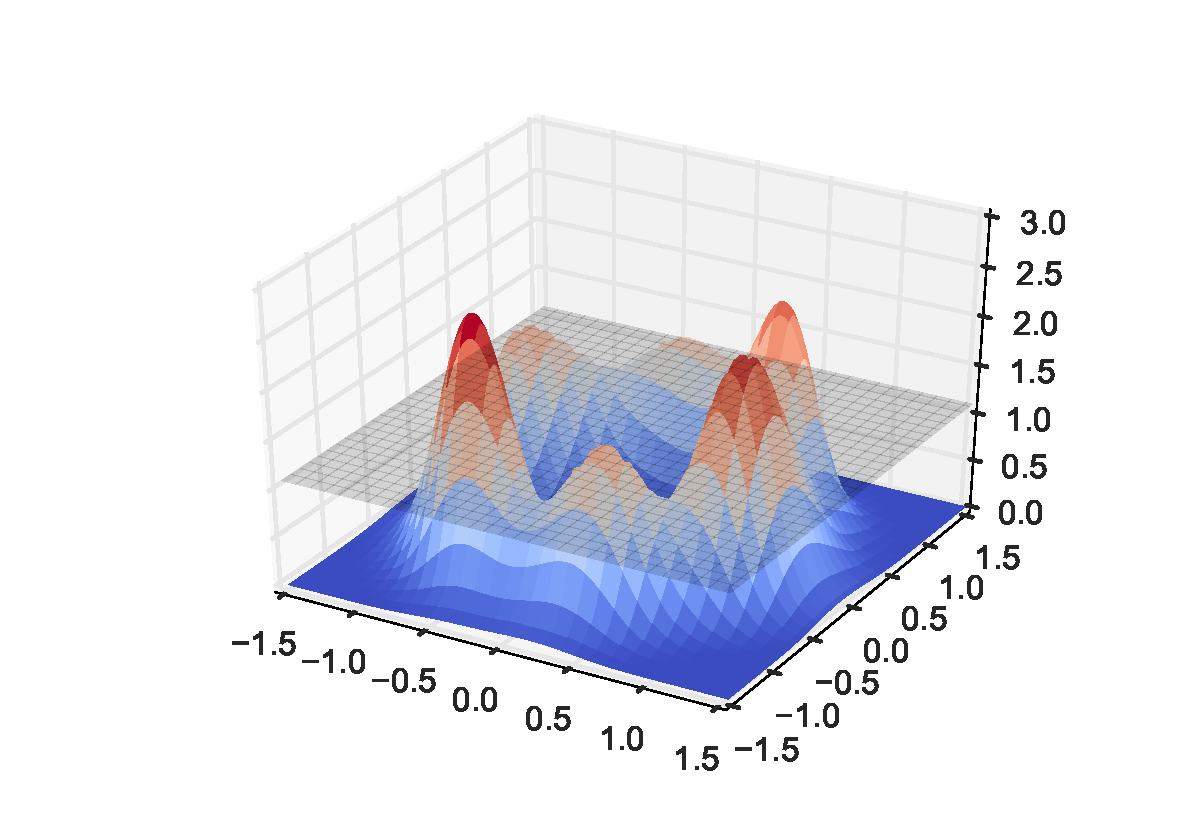
\includegraphics[width=\linewidth]{figure_2_3d_repr.pdf}
    \label{fig:example_3d}
  \end{subfigure}
    \begin{subfigure}{.25\linewidth}
    \centering
    \caption{}
        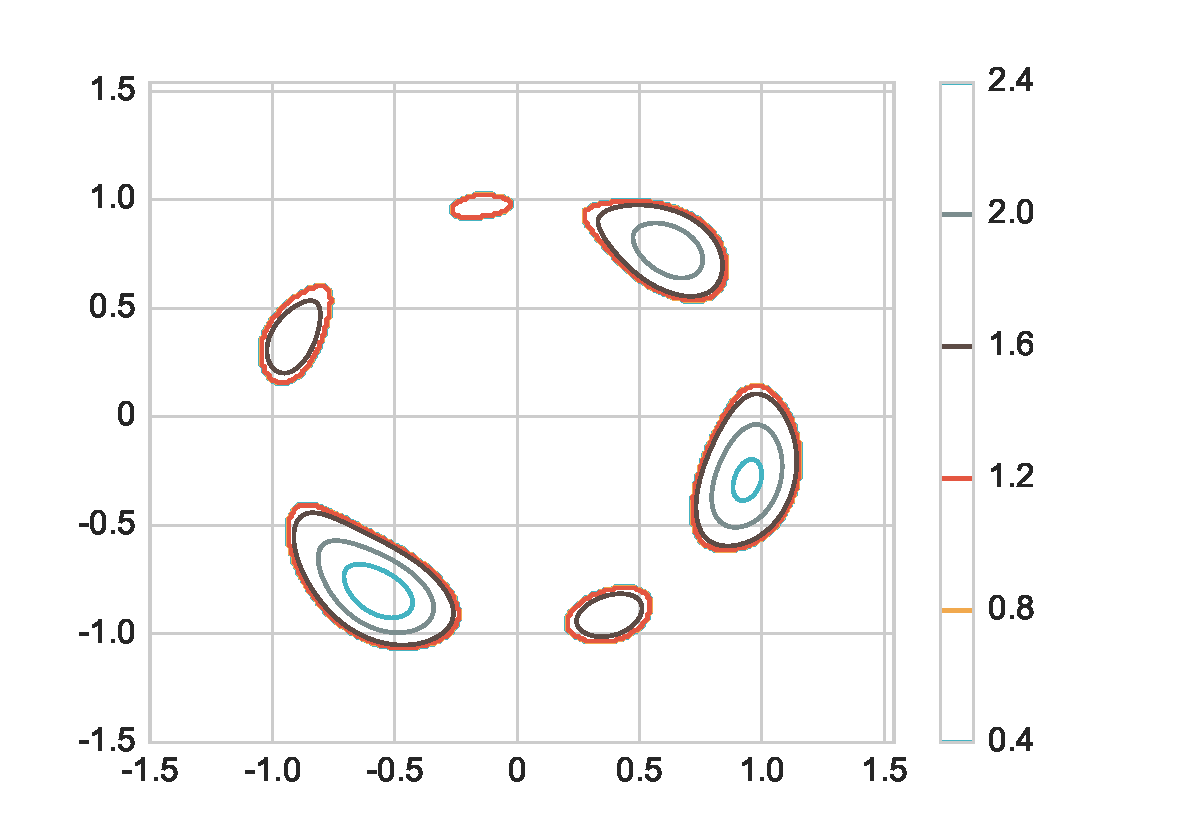
\includegraphics[width=\linewidth]{figure_2_contour_1.pdf}
    \label{fig:example_contour1}
  \end{subfigure}
    \begin{subfigure}{.25\linewidth}
    \centering
    \caption{}
        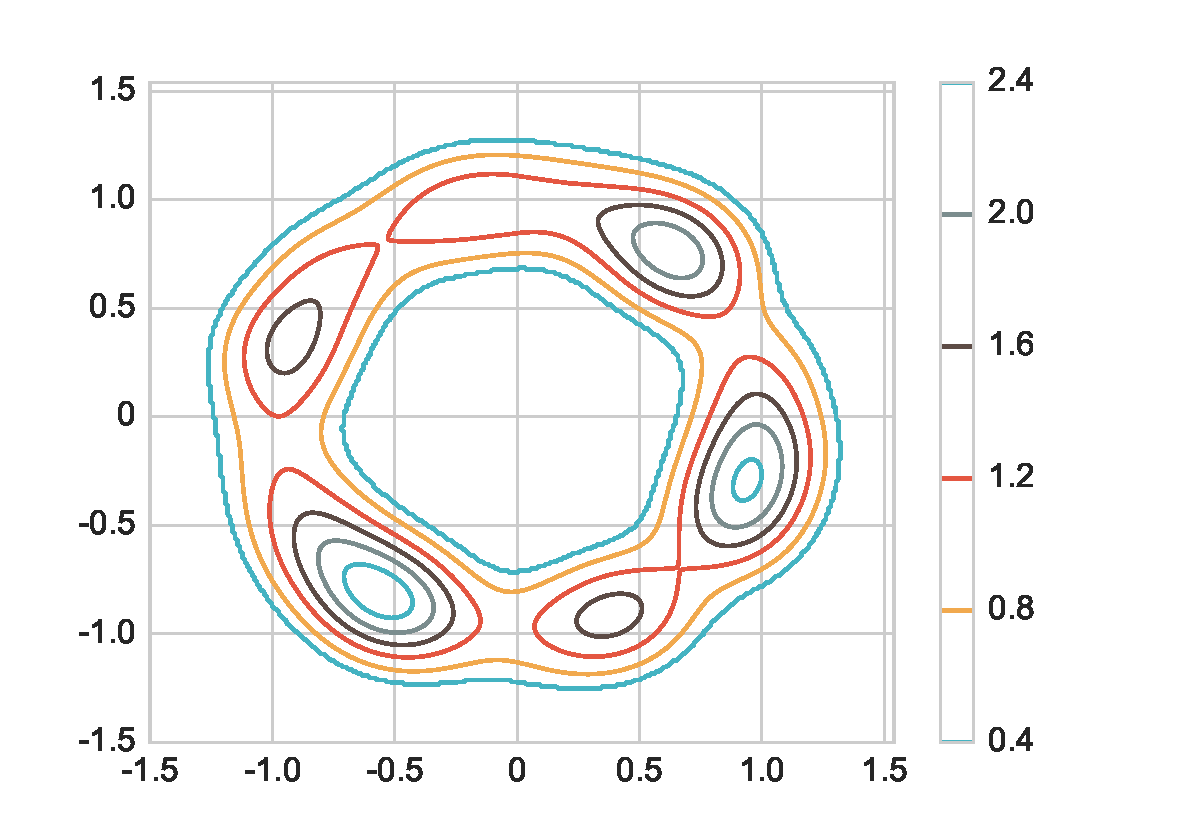
\includegraphics[width=\linewidth]{figure_2_contour_2.pdf}
    \label{fig:example_contour2}
  \end{subfigure}
    \begin{subfigure}{.20\linewidth}
    \centering
    \caption{}
        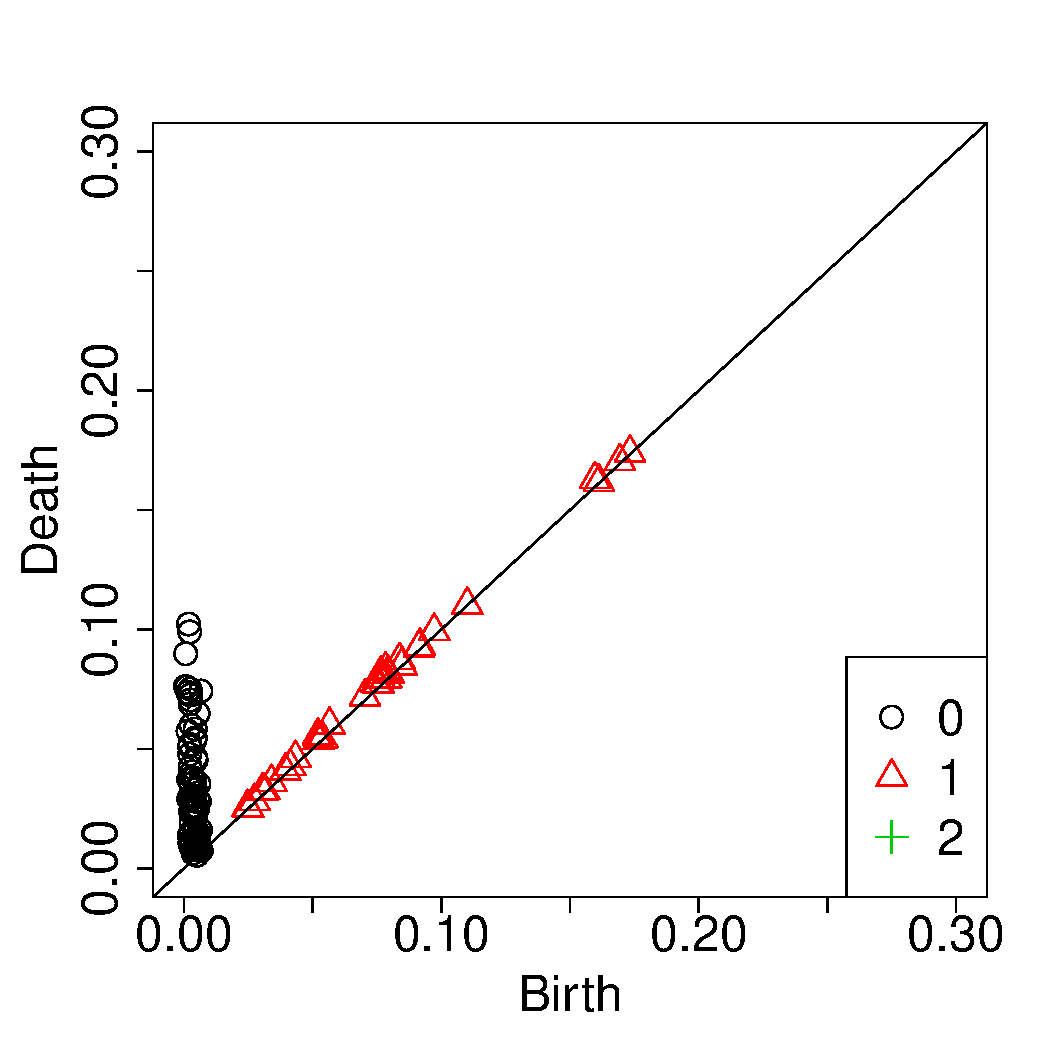
\includegraphics[width=\linewidth]{figure_2_pd.pdf}
    \label{fig:example_pd}
  \end{subfigure}
  \caption{ We illustrate persistent homology with this two-dimensional example. The density, $p$, in (a) shows 3 steep peaks and 3 shallow peaks  distributed around a circle. The gray hyperplane defines the threshold for super-level sets, and (b) and (c) plot the super-level sets $p^{-1}[1.10,\infty)$ and $p^{-1}[0.10,\infty)$ respectively. As the threshold decreases, the contour more clearly defines a loop-like structure. In (d), the persistence diagram for the super-level set filtration of $p$. We highlight the upper left quadrant based at $(0.18, 0.02)$, which contains an $H_1$ generator as a red triangle. The remaining 0-dimensional $H_0$ generators represent the connected components from each of the 6 peaks and are displayed as black circles.  There are no $H_2$ generators (green pluses).
  } % end caption
    \label{fig:homologyexample}
\end{figure}

%\paragraph{An Example}
%In order to illustrate persistent homology, we step down a dimension from cubes in $\R^3$ to squares in $\R^2$. In \figref{fig:homologyexample}, we see how persistent homology captures the evolving super-level sets of a KDE $\widehat{p} \colon [-2,2]^2 \to \R$.  The density plot in \figref{fig:homologyexample} was created using 6 Gaussian peaks distributed along a uniform circle in the $<x,y>$ plane. As the persistence parameter $t$, shown as a hyperplane in \figref{fig:homologyexample}(a), decreases from $\infty$ to $-\infty$, various events occur in the super-level sets $\widehat{p}^{-1}[t,\infty)$: a new component can appear (zeroth-dimensional birth), two distinct components can merge (zero-dimensional death), a loop can appear (one-dimensional birth), and two loops can become homologous (one-dimensional death).  These birth and death events are paired and plotted in the persistence diagram.
%%
%In the persistence diagram of \figref{fig:homologyexample}(a), we see exactly 6 zero-dimensional persistence points (denoted by black circles), one for each of the Gaussian peaks, and a single one-dimensional persistence point (denoted by red triangles), representing the circle on which the modes are located and is captured in \figref{fig:homologyexample}(c).
%
%The upper-left quadrant based at a point $(x,x)$ will contain all persistence points that are born before $x$ and die at or after $x$; that is, the persistence points in this quadrant are in one-to-one correspondence with generators of $p^{-1}(x,\infty)$.  In this way, the homology of each super-level set can be read off of the persistence diagram.
%\brittany{todo: continue here (update for new example)}

\subsection{Derivatives of Persistence Diagrams} \label{sec:derivatives}
While persistence diagrams are useful summaries of the topology of a data set, they are not easy to work with directly.
For example, the distance between two persistence diagrams can be calculated using, for example,  the bottleneck distance or the $q$-Wasserstein distance, but both are computationally expensive.
Fr\'echet means and medians have been defined for spaces of persistence diagrams \citep{Turner:2014kq}, but are also computationally expensive and not necessarily unique.  Instead we consider transformations and summaries of persistence diagrams that make computations more tractable.
Below are several approaches that further summarize a persistence diagram and will be used in \S \ref{sec:methods} to develop hypothesis tests.




%%%%%%%%%%%%%%%%%%%%
\paragraph{Weighted silhouette functions}
Weighted silhouette functions are formed by weighting a particular functional summary of persistence diagrams called \emph{landscape functions} \citep{bubenik2015statistical}.
Landscape functions are defined as follows. Let the finite birth and death intervals of a persistence diagram with $n_h$ points, for homology dimension $h = 0, 1, 2, \ldots$, be defined as $\{(b_{hi},d_{hi})\}_{i = 1}^{n_h}$.  Next, consider rotating the persistence diagram such that a given point is $p_{hi} = \left(\frac{b_{hi}+d_{hi}}{2}, \frac{d_{hi}-b_{hi}}{2}\right) \in D_h, \quad i = 1, \ldots, n_h$.  Equilateral triangles are formed from each $p_{hi}$ to the base as
\begin{equation*}
\Lambda_{p_{hi}}(t) =
  \begin{cases}
    t - b_{hi}  & \quad t \in [b_{hi}, \frac{d_{hi}+b_{hi}}{2}]\\
    d_{hi} - t  & \quad t \in [\frac{d_{hi}+b_{hi}}{2}, d_{hi}]\\
    0  & \quad \text{ otherwise}\\
  \end{cases}
\end{equation*}
where $t \in [t_{\min}, t_{\max}]$. For a given $h$, the persistence landscape is then defined as the following collection of functions
%
\begin{equation*}
\lambda_{D_h}(k, t) = \underset{p_{hi}\in D_h}{\text{kmax }} \Lambda_{p_{hi}}(t), \quad t \in [t_{\min}, t_{\max}], k = 1, \ldots, n_h
\end{equation*}
where kmax is the kth largest value in $D_h$.  An example of a persistence landscape function is displayed in Figure~\ref{fig:landscape}.

\begin{center}
\begin{figure}[htp!]
  \centering
%  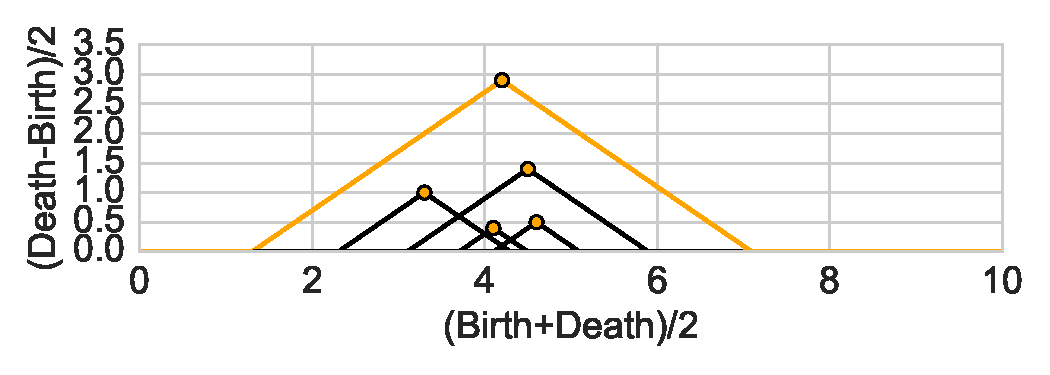
\includegraphics[width=0.6\linewidth]{figure_3_silh.pdf}
  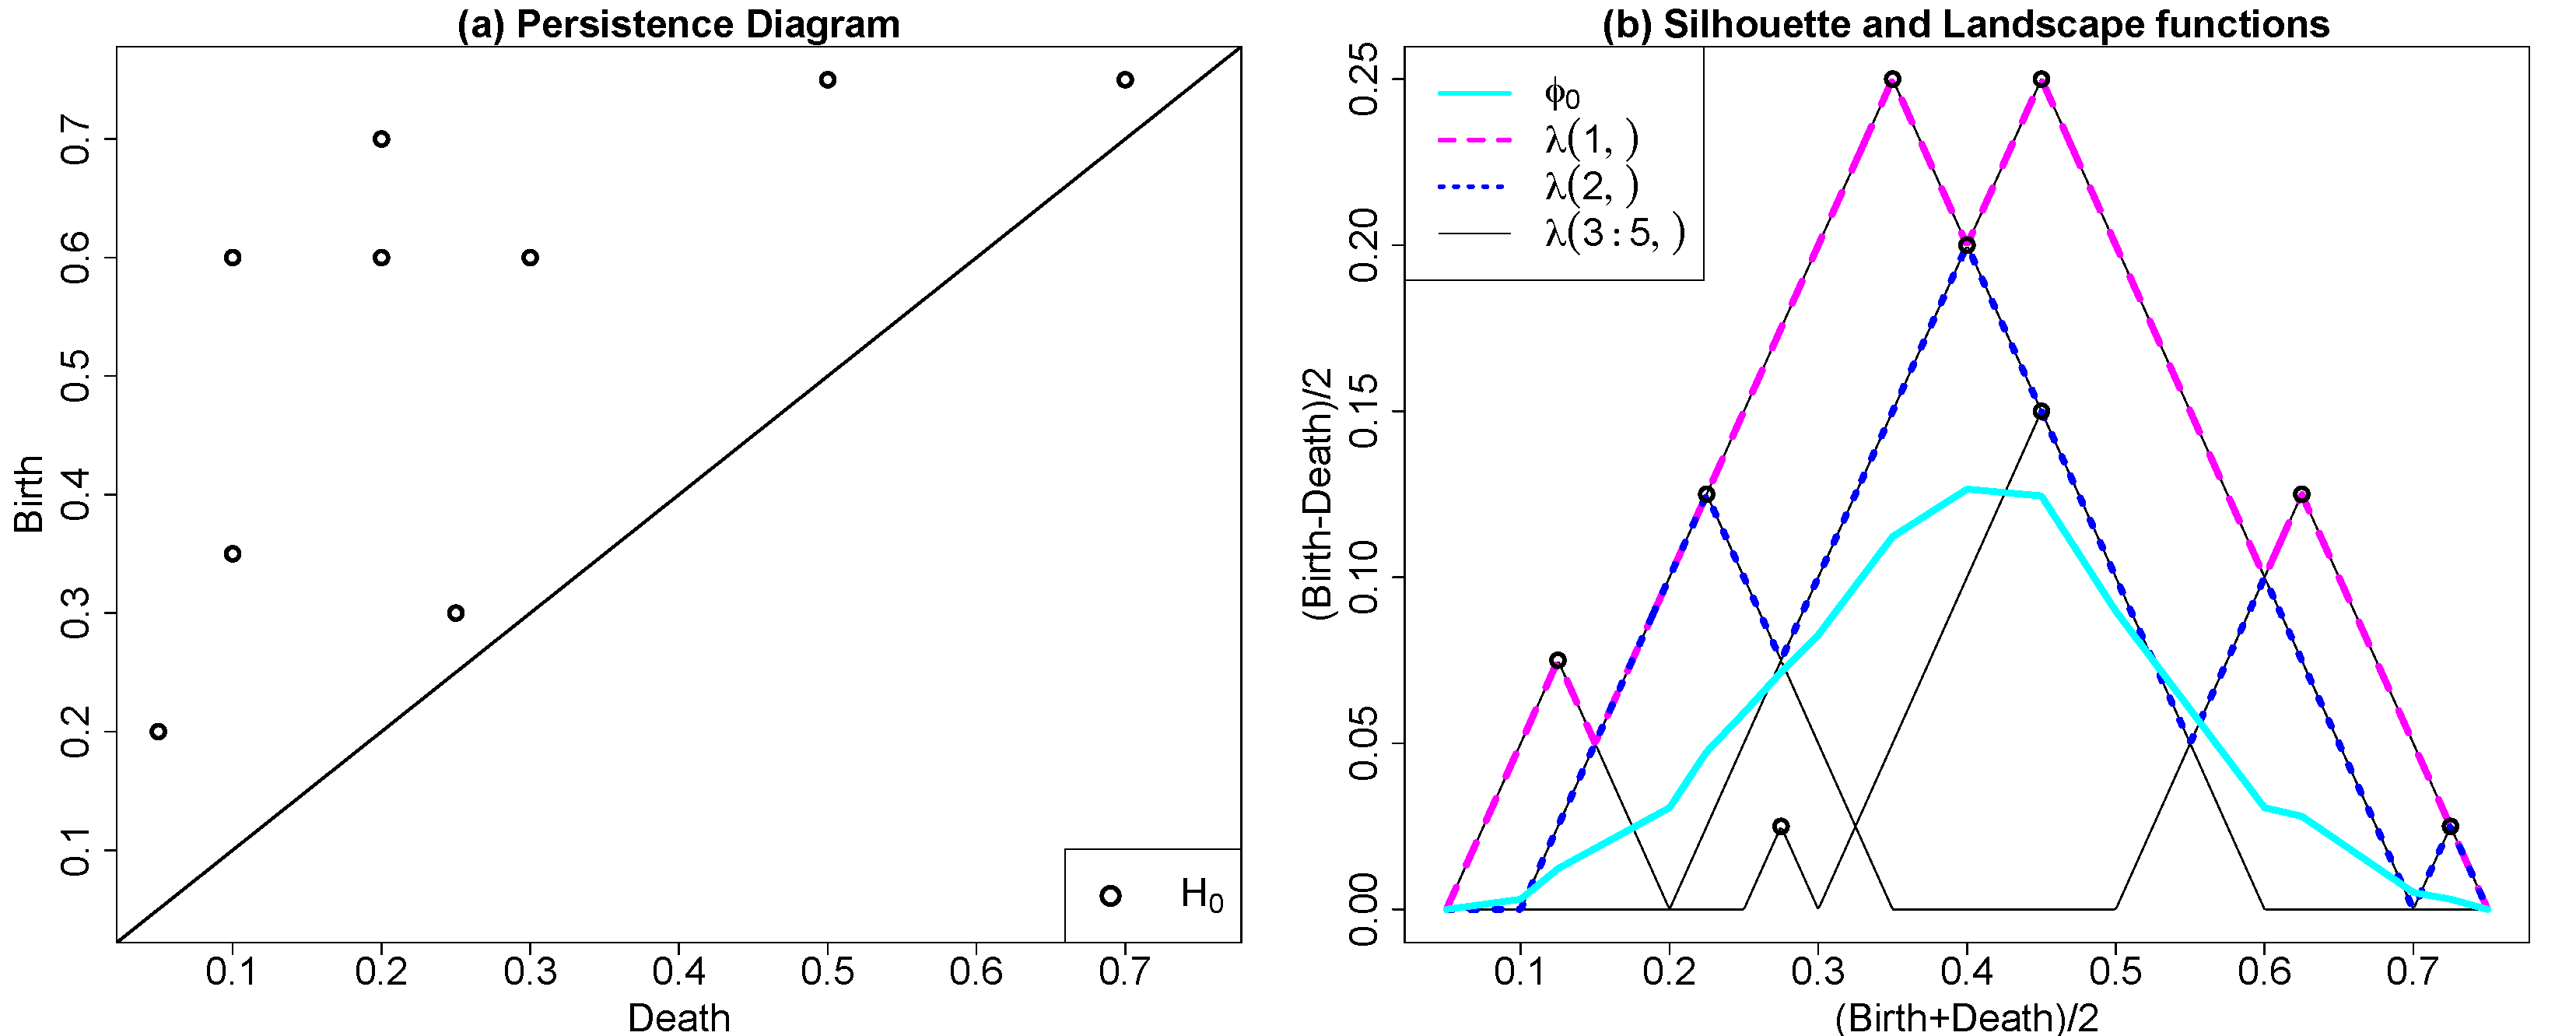
\includegraphics[width=0.95\linewidth]{fig_landscape_jjc.pdf}
    \caption{A persistence diagram (a) along with its silhouette and landscape functions (b) for $H_0$.  The solid cyan curve is the silhouette function with $p = 1$; the magenta dashed and blue dotted lines in (b) are landscape functions $\lambda_{D_0}(1, \cdot)$ and $\lambda_{D_0}(2, \cdot)$, respectively.}
    \label{fig:landscape}
\end{figure}
\end{center}

Rather than working with each $k$ of $\lambda_{D_h}(k, t)$ individually, weighted silhouettes provide a way of combining the information in the collection of landscape functions. Silhouettes are weighted averages of the individual functions for homology dimension $h$ defined~as
%
\begin{equation*}
\phi_h(t) = \frac{\sum_{i = 1}^mw_{hi}\Lambda_{hi}(t)}{\sum_{i = 1}^mw_{hi}}
\end{equation*}
where the weights $w_i$ can give more emphasis or less emphasis to features with longer lifetimes. As suggested in \citep{chazal2014stochastic}, we use $w_{hi} = |d_{hi} - b_{hi}|^p$, where $p$ is a tuning parameter that needs to be selected.  An example of a weighted silhouette function is provided in Figure~\ref{fig:landscape}.
More details and theoretical properties of landscapes and silhouettes are provided in \citep{chazal2014stochastic}.


%%%%%%%%%%%%%%%%%%%%
\paragraph{Euler Characteristic Function}
The Euler characteristic is a topological invariant and defined as: $\chi = \sum_{i=0}^{N} (-1)^{i} \beta_{i}$,
where $\beta_{i}$ represents the $i$-th Betti number (the rank of the $i$-th homology group) and $N$ is the number of dimensions. When analyzing persistence diagrams of LSS, since there exist only three dimensions of data, the only non-trivial homology groups will be in dimensions 0, 1, and 2. Given the Betti numbers $\beta_{0}$, $\beta_{1}$, and $\beta_{2}$, the Euler equation simplifies to:
$\chi = \beta_{0} - \beta_{1} + \beta_{2}.$
As the filtration threshold $t$ decreases and new features are born or old ones die, the Euler Characteristic changes so we consider the Euler Characterisitic function, $\chi(t)$, $t \in [t_{\min}, t_{\max}]$.



%%%%%%%%%%%%%%%%%%%%
\paragraph{Smooth Persistent Diagrams}
Another variation of persistent diagrams are smoothed persistence diagrams. \cite{chen2015statistical} introduced \emph{persistent intensity functions}, which is a weighted kernel density estimate of a persistence diagram with weights as a function of a point's persistence. Let $\mathcal{D} = {(b_i , d_i) : i = 1, \cdots ,m}$ be a persistence diagram where $m$ is the number of persistent features for dimension $h$.  Then the weighted intensity function for the persistence diagram is
%
\[ X(t_1, t_2) = \sum_{j=1}^m(d_{j} - b_{j})\frac{1}{\tau^{2}}K \left(\frac{t_1-d_{j}}{\tau}\right)K \left(\frac{t_2-b_{j}}{\tau}\right)\]
%
for $t_{\min} \leq t_1 \leq t_2 \leq t_{\max}$ with symmetric kernel function $K$, and smoothing parameter $\tau$.  An example of a persistent intensity function is displayed in Figure~\ref{fig:examplestest5}.

\emph{Persistent Images} are similar to persistent intensity functions \citep{adams2015persistent} except that the persistence diagram is rotated and the smoothed diagram is pixelized into a uniformly spaced 2-dimensional grid of a chosen resolution, and finally vectorized.   The persistence diagram is transformed using the linear transformation $T: \mathbb{R}^{2} \rightarrow \mathbb{R}^{2}$ where $T(x,y) = (x, y-x)$; therefore $T(\mathcal{D})$ represent the transformed diagram with birth-persistence coordinates.  As with persistent intensity functions, the now transformed diagram is smoothed using weighted kernel density estimation, with weights that are zero on the horizontal axis.  \cite{adams2015persistent} use a piecewise, linear weighting function that assigns a weight of 0 to points with 0 persistence.
A 2-dimensional grid is then defined over the smoothed $T(\mathcal D)$ to turn it into a matrix of a user-selected resolution.  The matrix is then vectorized and easily used as inputs into a statistical analysis.   See Figure~\ref{fig:examplestest8} for an example of a persistent image.



\begin{figure}[htbp]
  \centering
  \begin{subfigure}{0.22\textwidth}
    \centering
      \caption{Point Cloud}
      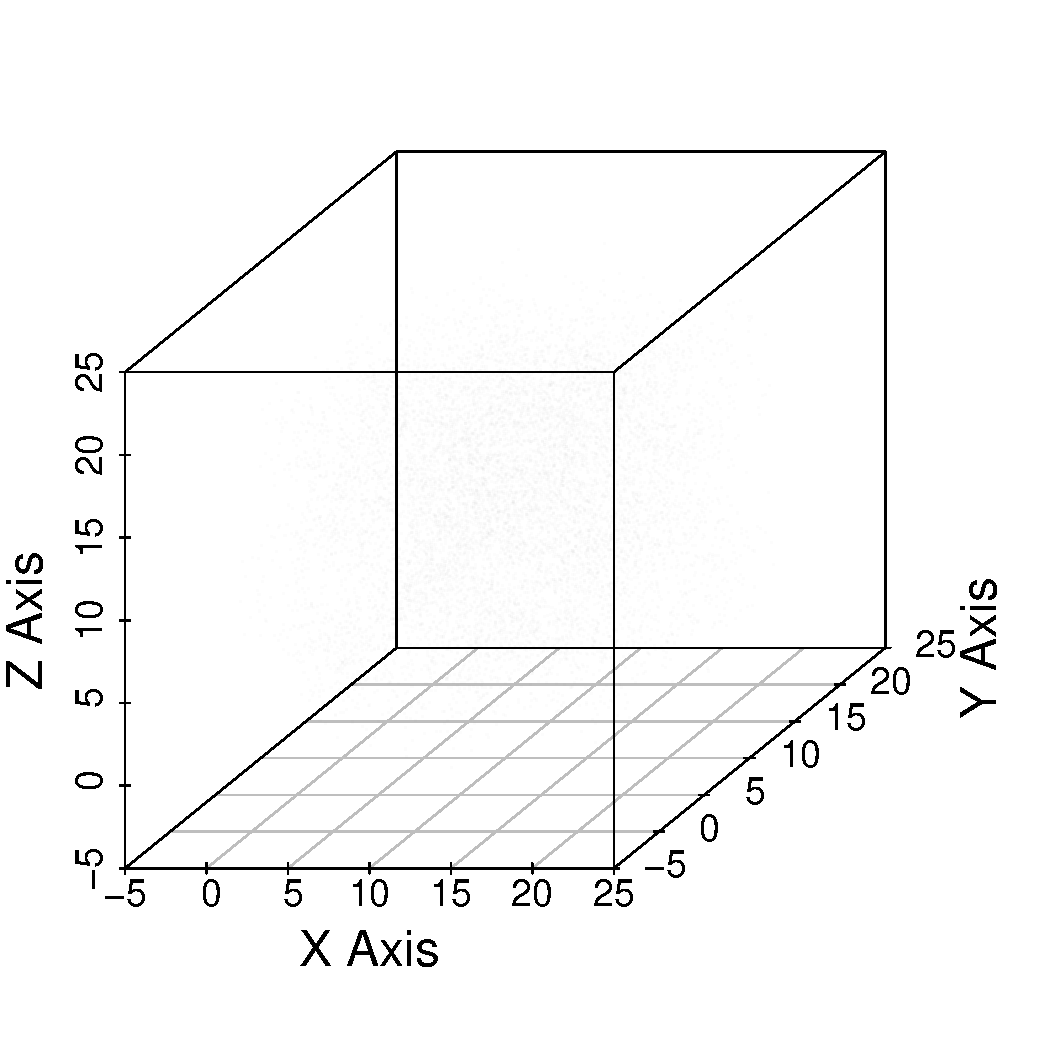
\includegraphics[height = 1.15in]{figure_5_plot.pdf}
    \label{fig:examplestest1}
  \end{subfigure}
  \begin{subfigure}{0.22\textwidth}
    \centering
        \caption{Persistence Diag}
        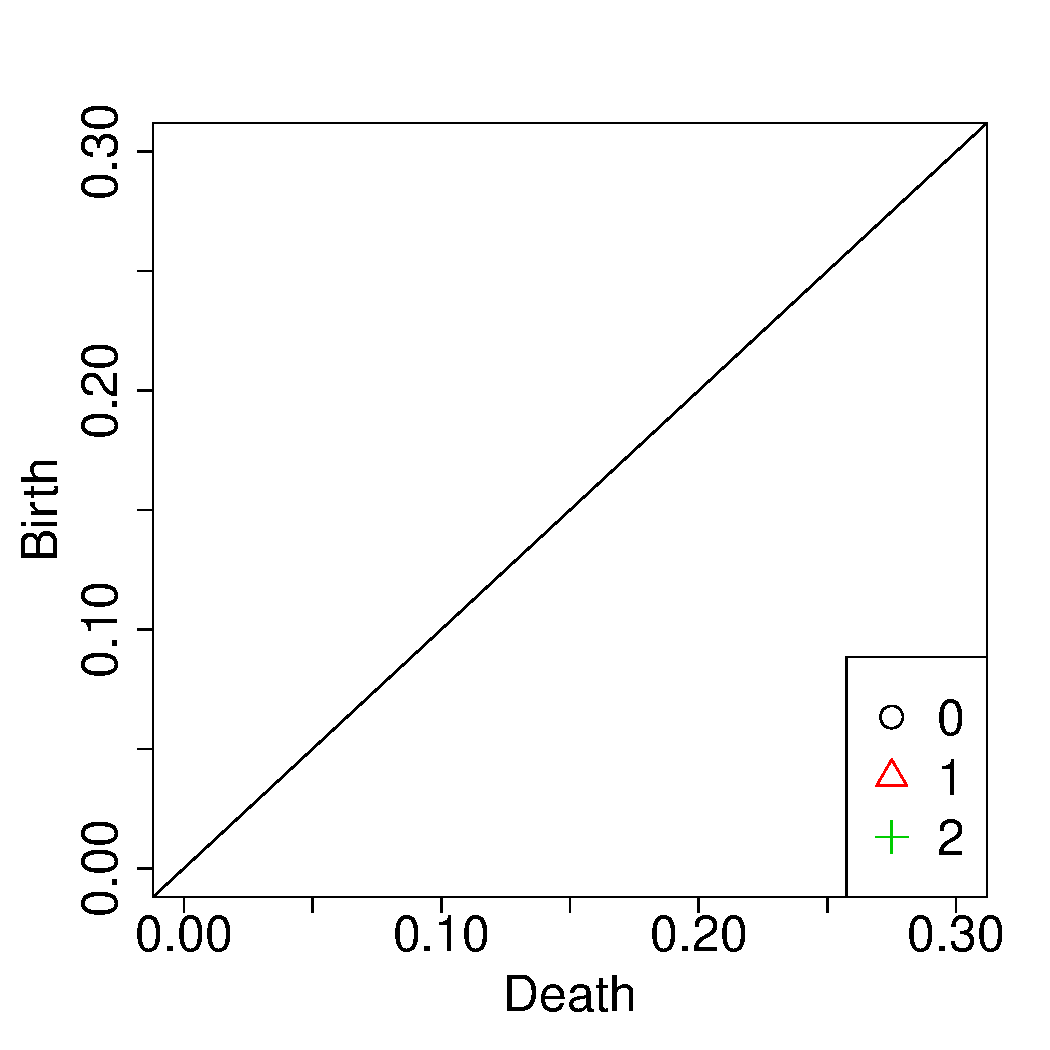
\includegraphics[height = 1.15in]{figure_5_pd.pdf}
    \label{fig:examplestest2}
  \end{subfigure}
  \begin{subfigure}{0.26\textwidth}
    \centering
        \caption{Intensity Func.}
        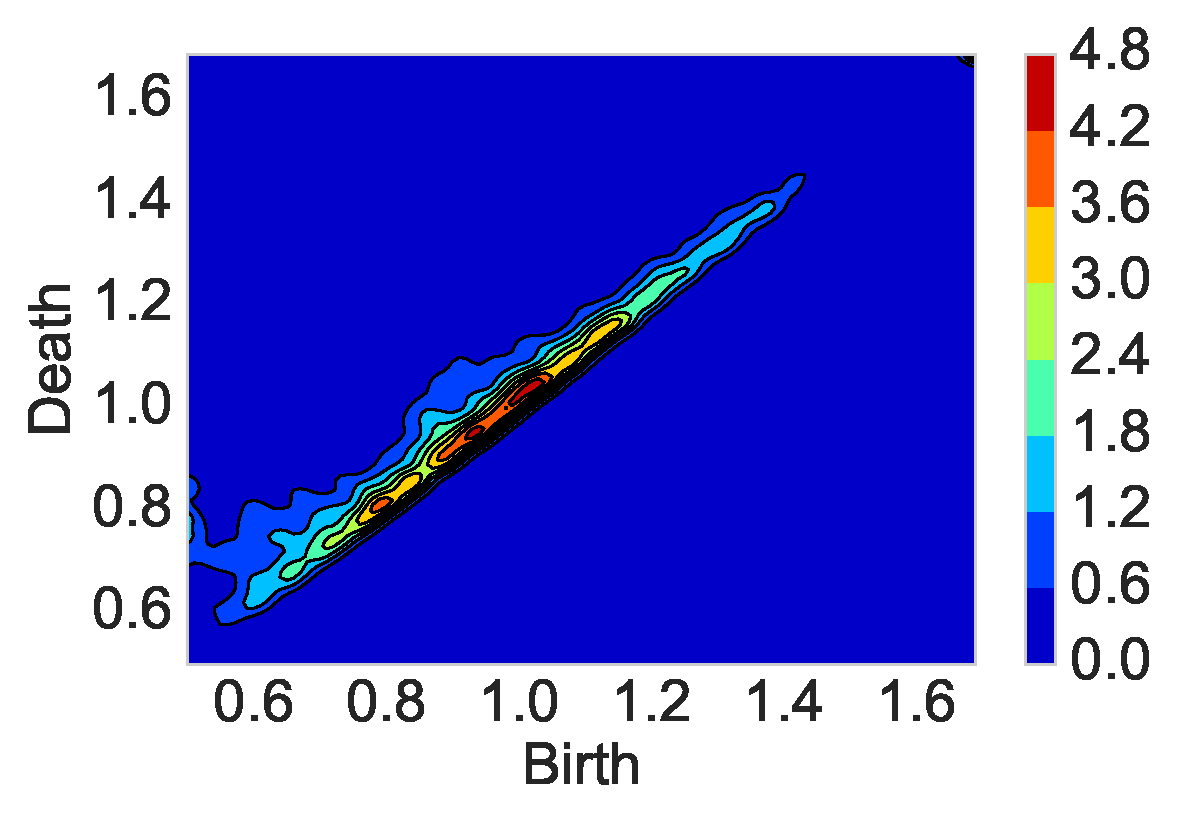
\includegraphics[height = 1.11in]{figure_5_kernel.pdf}
    \label{fig:examplestest5}
  \end{subfigure}
  \begin{subfigure}{0.26\textwidth}
    \centering
        \caption{Persistent Image}
        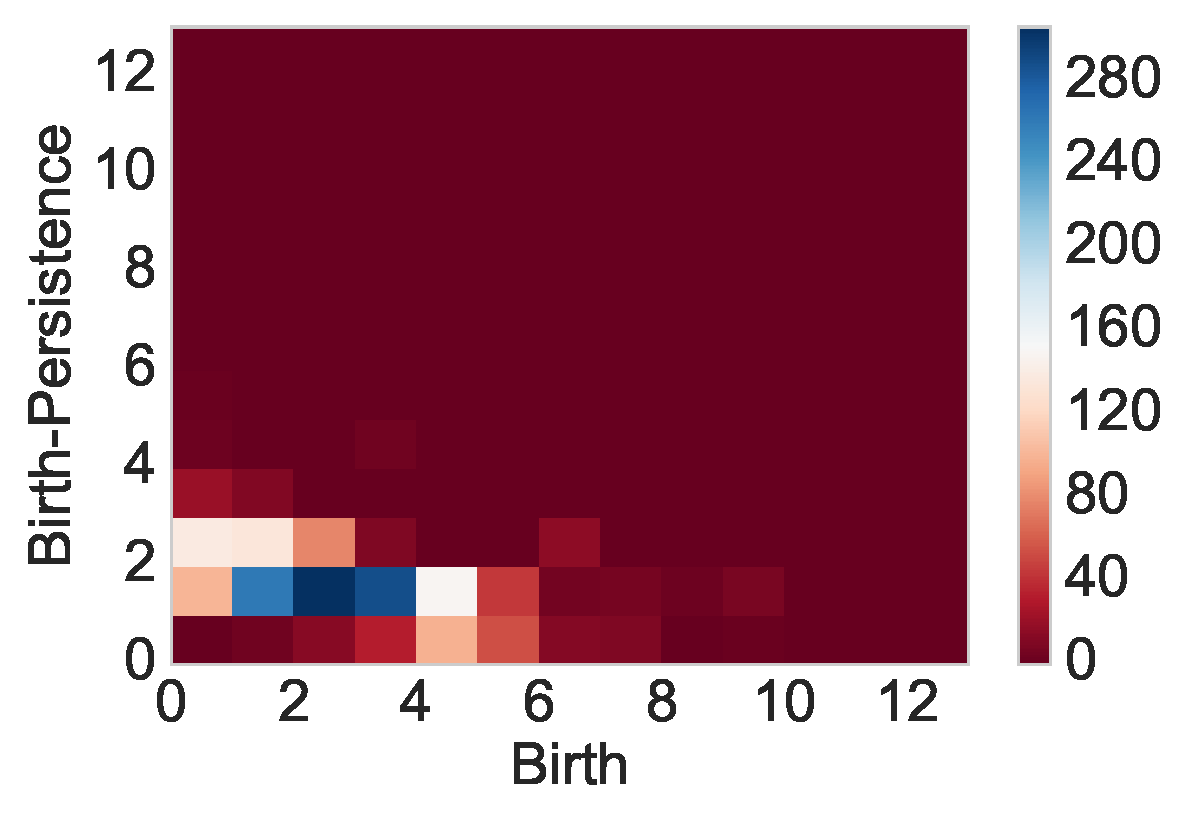
\includegraphics[height = 1.11in]{figure_5_pimage_fun.pdf}
    \label{fig:examplestest8}
  \end{subfigure}
  \caption{Examples of smoothed persistence diagrams.  A 3-dimensional point cloud is provided in (a) along with its persistence diagram in (b).
The Persistence Intensity function in (c) and Persistence Image in (d) are both for $H_0$,
See \S \ref{sec:methods} for more details.}
   \label{fig:examples}
\end{figure}







%%%%%%%%%%%%%%%%%%%%%%%%%%%%%%%%%%%%%%%%%%%%%%%%%%%%%%%
%% SECTION: METHODS
%%%%%%%%%%%%%%%%%%%%%%%%%%%%%%%%%%%%%%%%%%%%%%%%%%%%%%%

\section{Methods} \label{sec:methods}
\begin{sloppypar}
Using the variations of persistence diagrams described in \S \ref{sec:derivatives},
we describe several options for test statistics for two-sample hypothesis tests for topological structure.
For this setup, suppose we have two sets of persistence diagrams, $\{\mathcal P_1^{(1)}, \ldots, \mathcal P_{n_1}^{(1)}\}$ and $\{\mathcal P_1^{(2)}, \ldots, \mathcal P_{n_2}^{(2)}\}$.  These samples can be used to test $H_0: \mathcal
P^{(1)} = \mathcal P^{(2)}$ vs. $H_1: \mathcal P^{(1)} \neq \mathcal P^{(2)}$, where $\mathcal P^{(1)}$ and $\mathcal P^{(2)}$ are the true underlying distributions of persistence diagrams.  Probability measures can be defined on a space of persistence diagrams (with a Wasserstein metric) as presented in \citep{Mileyko:2011aa}. We would like the framework to test the hypothesis that the two samples are drawn from populations with different random topologies. However, we note that without incorporating a scaling adjustment on the space  of the data or the space of the diagrams, geometrical differences can also lead to a rejection of the null hypothesis. This is discussed in more detail in \S \ref{sec:standardize}.
\end{sloppypar}

Given two samples of persistence diagrams, there are a number of possible ways to derive test statistics. We consider functional versions of persistence diagrams as test statistics:  the Euler characteristic function, Silhouette function, and a Silhouette-Euler characteristic function (which will be defined below).
Given that each observed dataset will have a corresponding functional summary, a \emph{p-value} can be derived from a two-sample T-test by integrating the absolute value of the functional summary.
We consider persistent intensity functions and persistent images with p-values derived from a two-sample kernel test statistic \citep{gretton2012kernel}, and use a permutation test to get a p-value.
%
Additionally, we consider a test using the two-point correlation function.  The correlation function is used to capture the spatial behavior of LSS, and we include it to see if the differences in LSS can be attributed to spatial differences rather than topological differences.
As with the functional summaries above, p-values are calculated with a T-test using the integral of the absolute value of the correlation function.

The proposed test statistics are discussed in more detail below.  Among the proposed test statistics, we are seeking the summary that is most sensitive to differences in distributions of persistence diagrams produced from LSS.

% Given any persistence diagram $x$ extracted from a point cloud, $x$ represents a sample from some latent distribution $\chi$. For example, given a simulation of the Megaparsec cosmic mass, the $(x, y, z)$ points are discrete samples from the continuous, observable Universe, which represents the true distribution. Using that definition, suppose there are two persistence diagrams, $x$ and $y$, each produced from a separate point cloud. Given that $x \sim \chi$, and $y \sim \gamma$, where $\chi$ and $\gamma$ represent the true distributions, an interesting question is whether $\chi$ and $\gamma$ are identical to some error $\epsilon$. In other words, are the samples $x$ and $y$ sampled from the same latent distribution? One might consider the following hypothesis test, where $H_{0}$ is the null and $H_{A}$ is the alternative.

% \[ H_{0} : \chi = \gamma \]
% \[ H_{A} : \chi \neq \gamma \]

% However, given that the parameters of the distributions $chi$ and $\gamma$ are unknown, one cannot directly compare them. Instead, one much infer the relationship between $chi$ and $gamma$ by comparing the diagrams sampled from $\chi$ and $\gamma$ respectively. Given $n$ samples, a hypothesis test should be designed to compare $\{ x_{1}, ..., x_{n} \sim \chi \}$ and $\{ y_{1}, ..., y_{n} \sim \gamma \}$. However, comparing two persistence diagrams, $x$ and $y$, is non-trivial. Naive distance calculations, like bottleneck or Wasserstein, are easily perturbed by randomness and noise, and are computationally expensive. Instead, we propose to further summarize a persistence diagram by a test statistic. To find such a test statistic, we must define a function $f_{T}$ that takes an input $x$ and produces a statistic $T_{x}$, $f_{T}(x) = T_{x}$. Provided such a function exists, using the further summarized statistics, we can test the hypothesis that two persistence diagrams, $x$ and $y$ are sampled from the same latent distribution with the following framework:

% \[ H_{0} : f_{T}(x) = f_{T}(y) \]
% \[ H_{A} : f_{T}(x) \neq f_{T}(y) \]

% One main contribution of this paper is studying the effectiveness of different functions $f_{T}$ when the true topological relationship between $x$ and $y$ are known. The best functions $f_{T}$ are then used to analyze a data set in which the topological relationships is unknown. We now proceed to describe different methods for defining $f_{T}$ for hypothesis testing in the setting of large-scale structure (LSS).



\paragraph{Euler Characteristic Test (EC)}
Each persistence diagram in the two samples result in an individual Euler characteristic function, $\chi^{(J)}(t)$,  $J = 1, 2$. The two-sample T-test is based on the sample means
$
\bar{EC}_J = \frac{1}{n_J}\sum_{i = 1}^{n_J} \int_{t_{\min}}^{t_{\max}} | \chi_i^{(J)}(t) | \textup{ d}t.
$
Note that the Euler characteristic function combines all homology dimensions into a single functional summary.


% \begin{center}
% \begin{figure}[htp!]
%   \centering
%   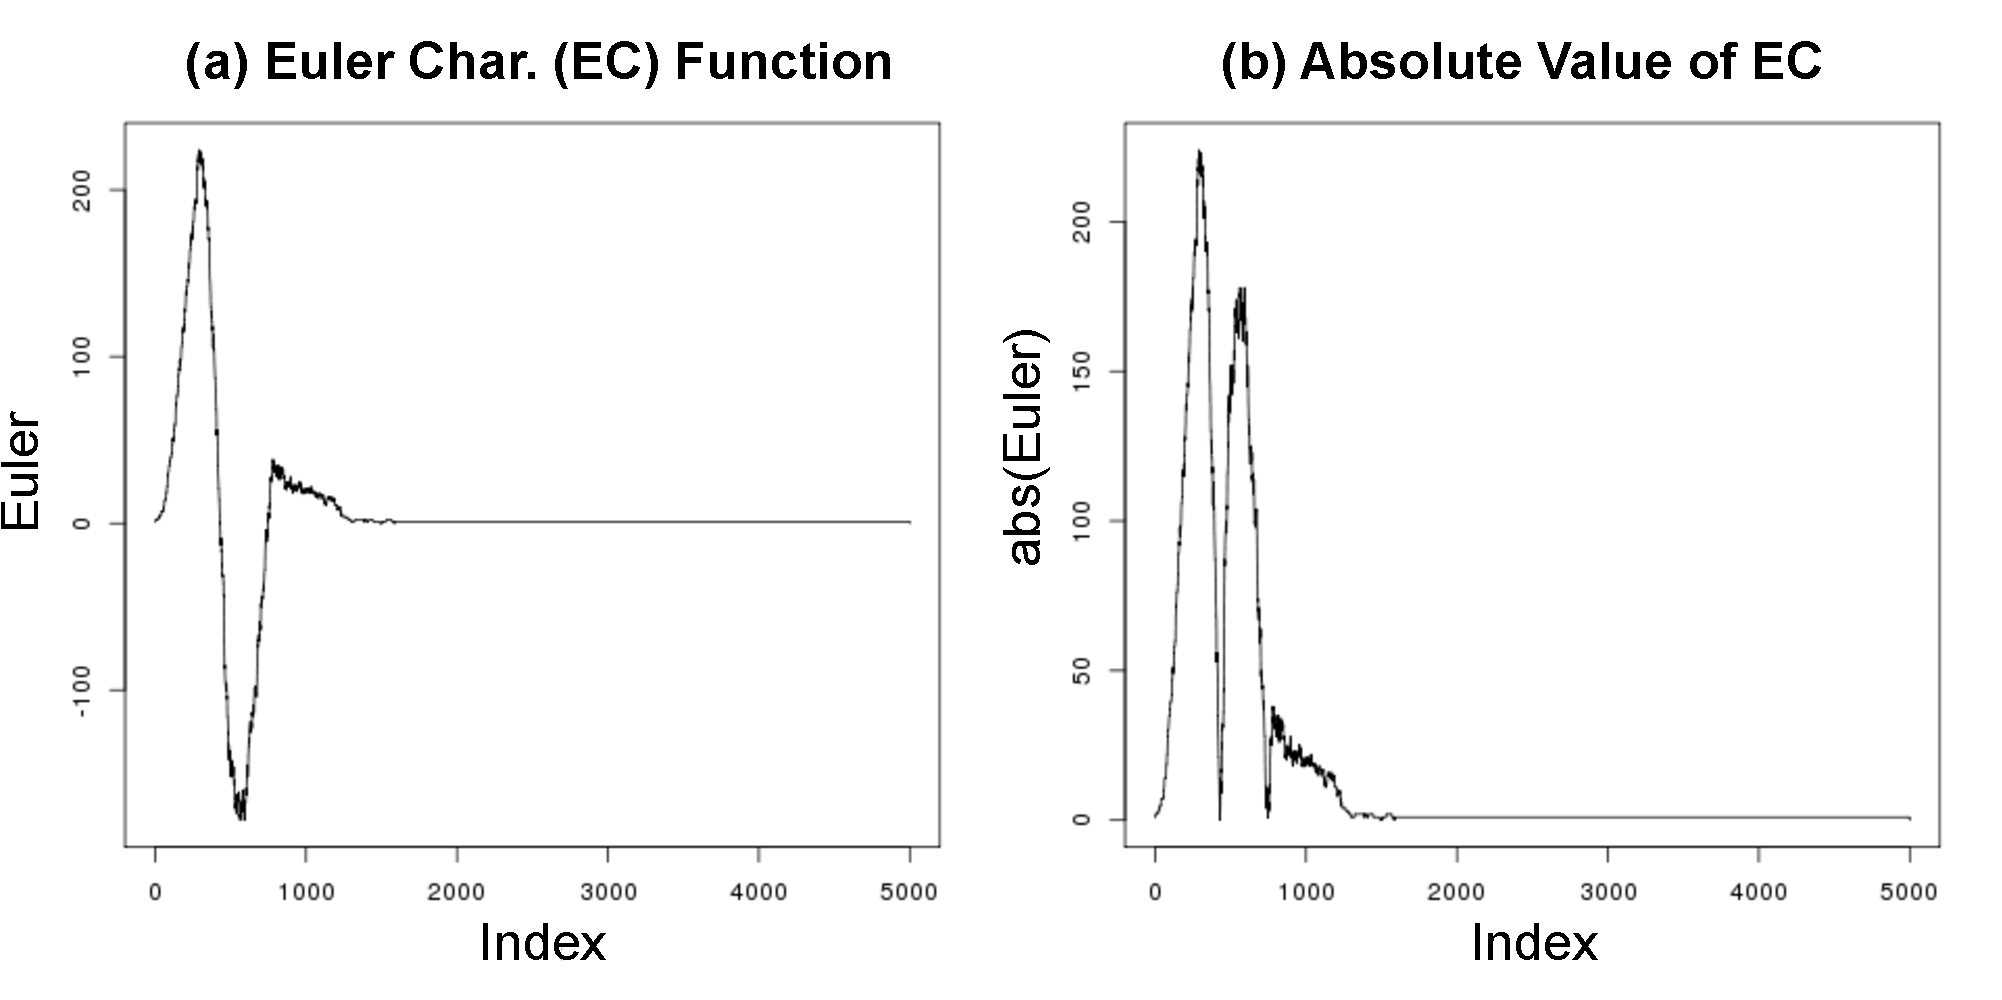
\includegraphics[width=0.7\linewidth]{example_euler.pdf}
%     \caption{(a) An Euler characteristic function created by plotting the Euler characteristic of a Voronoi foam model at each point beginning at time 0 until the last birth time. (b) The absolute value of the characteristic function that is integrated to produce the test statistic $E_{t}$.}
%     \label{fig:eulerexample}
% \end{figure}
% \end{center}

\paragraph{Silhouette Test (SIL)}
As with EC, the Silhouette Test (SIL) is a two-sample T-test is carried-out by integrating the weighted silhouette functions for each sample $J = 1, 2$ and each homology dimension $h = 0, 1, 2$:  $
\bar{SIL}_{hJ} = \frac{1}{n_J}\sum_{i = 1}^{n_J} \int_{t_{\min}}^{t_{\max}} | SIL_i^{(J)}(t) | \textup{ d}t.$  The SIL tests for homology dimension $h = 0, 1, 2$ are denoted, $SIL_0, SIL_1,$ and $SIL_2$, respectively.
In order to combine information across homology dimension, we use a Hotelling's $T^2$ test with all three dimensions, denoted $SIL_{0:2}$.


\paragraph{Silhouette-Euler Characteristic (SILEC).}
Another method for simultaneously considering individual silhouettes, $S_{h}(t)$, across dimensions $h = 0$, 1, and 2, is a modified Euler characteristic function. Instead of calculating the alternating sum of Betti numbers, the Silhouette-Euler characteristic function (SILEC) computes the alternating sum of silhouette functions across the threshold parameter, $t$, $SILEC(t) =  S_{0}(t) - S_{1}(t) + S_{2}(t)$. A p-value is calculated using a T-test in the same fashion as done for EC.




%\paragraph{Permutation Method.} Although not one of the nine approaches, the permutation method is frequently used in our tests and provides a very generic approach for calculating a p-value from any arbitrary test statistic. Assuming we observe two independent samples $X_{1}, \cdots, X_{n} \sim P$ and $Y_{1}, \cdots, Y_{n} \sim Q$, the two sample test problem is to test the hypothesis $H_{0} : P = Q$ versus the alternative $H_{1} : P \neq Q$. Assuming there is some arbitrary method of calculating a test statistic $T$ as a function of the data, we reject $H_{0}$ if $T > t$ where $t$ is a critical value. We choose $t$ such that if $H_{0}$ is true then $W(T > t) \leq \alpha$ where $W$ is the distribution of $T$ when $H_{0}$ is true. Permutation testing attempts to help us choose $t$ and find $W$ of $T$ under $H_{0}$.
%
%In the permutation method, the data is concatenated as a vector in the order \[X_{1}, X_{2}, \cdots, X_{n}, Y_{1}, Y_{2}, \cdots, Y_{n}\] and presented initial labels of $0$ or $1$ where all $X_{i}$ receive label 0 and all $Y_{i}$ receive label 1. If $H_{0}$ is true, then the entire data vector is an i.i.d sample from $P$ and the group labels are arbitrary. To test this, the group labels are randomly permuted and the test statistic is recalculated. This changes the values of $T$ but (under $H_{0}$), it should not change the distribution of $T$. The labels are permuted $N$ times and the p-value is
%
%\[ p = \frac{1}{N}\sum^{n}_{j=1} I(T_{j} \geq T) \]
%
%where $I$ is the indicator function. Therefore, the p-value is the fraction of times $T_{j}$ is larger than $T$. As $N$ approaches $\inf$, $p$ approaches the exact value.

\paragraph{Intensity Kernel Test (IK).}
The Intensity Kernel Test (IK) uses persistent intensity functions rather than the raw persistent diagrams.
The IK statistic used in this paper is computed for two sets of persistence diagrams, and the discrepancy between the diagrams is calculated as the integrated squared difference between two \emph{unweighted} intensity functions instead of points directly from the persistence diagrams. Unweighted intensity functions assigns uniform weights to points on the diagram and therefore does not account for the diagonal boundary on persistence diagrams where birth = death; we considered the usual weighted intensity functions as defined in \cite{chen2015statistical} in the Weighted Intensity Kernel Test discussed below.

 The two-sample test statistic for $X = X_1, \ldots, X_{n_1}$ and $Y = Y_1, \ldots, Y_{n_2}$ is defined using the two-sample Kernel Test from \cite{gretton2012kernel}:
%
\begin{equation}
\widehat{T}_{IK}(X, Y) = \frac{1}{n_1^{2}}\sum_{i=1}^{n_1}\sum_{j=1}^{n_1} K_{\sigma}(X_{i}, X_{j}) - \frac{2}{n_1n_2}\sum_{i=1}^{n_1}\sum_{j=1}^{n_2}K_{\sigma}(X_{i}, Y_{j}) + \frac{1}{n_2^{2}}\sum_{i=1}^{n_2}\sum_{j=1}^{n_2} K_{\sigma}(Y_{i}, Y_{j}), \label{eq:kernel_test}
\end{equation} where $n_1$ and $n_2$ are the sizes of the two samples, and $\{X_1, \ldots, X_{n_1}\}$ and $\{Y_1, \ldots, Y_{n_2}\}$ are the two sets of intensity functions.  $K_{\sigma}(X,Y)$ can be thought of as a similarity measure between intensity functions $X$ and $Y$, and in this case is a Gaussian kernel $K_{\sigma}(X,Y) = exp(-\frac{||X - Y||^{2}}{\sigma^{2}})$ with  $||X - Y|| = \sqrt{\int \left(X(t_1, t_2) - Y(t_1, t_2)\right)^2dt_1dt_2}$. The $\sigma$ is a hyperparameter that sets the standard deviation of the Gaussian distribution used in the kernel $K_{\sigma}$: a larger $\sigma$ will reduce sensitivity to small differences between $X$ and $Y$, while a smaller $\sigma$ will heighten sensitivity. The optimal $\sigma$ value was found to be $0.1 \pm 0.04$ using grid search from 0 to 5. A permutation test is used to calculate a p-value for each homology dimension, $IK_0$, $IK_1$, and $IK_2$.
% with $N$ permutations, and the p-value represents the fraction of times $T_{j}$ is larger than the observed $\widehat{GC}$ for any $j$,

% \[ \text{p-value} = \frac{1}{N} \sum_{j=1}^{N} I(T_{j} \geq T). \]

\paragraph{Weighted Intensity Kernel Test (WIK)}
The intensity function in WIK, unlike IK, uses weighted kernel density estimates \citep{chen2015statistical} where the weights are a function of a feature's persistence. 
Using weighted intensity functions, a p-value is calculated by considering the same kernel test statistic as Equation~\eqref{eq:kernel_test}. A permutation test for each homology dimension produces three analogous statistics: $WIK_0$, $WIK_1$, and $WIK_2$.






\paragraph{Persistent Image Test (PI)}   The Persistent Image Test (PI) uses the Persistent Image transformation of persistent diagrams introduced in \cite{adams2015persistent}. The dimension of the persistent image is $10 \times 10$ resulting in a vector of length 100.  Unlike the WIK test, the PI test combines all homologies into a single statistic by concatenating the vectors for each homology dimension.
A p-value is calculated using the two-sample kernel test statistic from Equation~\eqref{eq:kernel_test} along with permutation test.



\paragraph{Two-point Correlation Function Test (CORR)} 
The Two-Point Correlation Function Test (CORR) considers to the two-point correlation function of the raw data in order to compare the persistent homology tests with a test based on the spatial distribution of the LSS.  The two-point correlation function was selected due to its ubiquitous employment in the astronomy literature (e.g. \citealt{Baugh:2006aa, Sanchez:2012aa}), and provides a measure of the degree of clustering in a dataset.   
The implementation used to get the two-point correlation function is from the Python {\tt TreeCorr} library \citep{jarvis2004skewness, Jarvis:2015aa}. 
As with the other function-based test statistics (where the two-point correlation function is a function that takes distances between points in the raw data as the input), the two-sample T-test is based on the sample means is used for CORR.
%$
%\bar{CORR}_J = \frac{1}{n_J}\sum_{i = 1}^{n_J} \int_{0}^{r_{\max}} | \xi_i^{(J)}(r) | dr.
%$





%%%%%%%%%%%%%%%%%%%%%%%%%%%%%%%%%%%%%%%%%%%%%%%%%%%%%%%
%% SECTION: SIMULATION STUDY
%%%%%%%%%%%%%%%%%%%%%%%%%%%%%%%%%%%%%%%%%%%%%%%%%%%%%%%

\section{Simulation Study}
\label{sec:simulation}

To evaluate the performance of the proposed test statistics, we carried out a simulation study by generating realizations of web-like spatial structures.  The simulation model is discussed in detail below.

\subsection{Simulation model} \label{sec:sim_model} %--------------------------------------
Motivated by LSS, we developed our simulation model to approximate the Cosmic Web. In particular, we drew from ideas that use Voronoi tessellations to model the filament structure of the Universe, known as \emph{Voronoi Foam} \citep{icke1987fragmenting, icke1991galaxy, van2007voronoi}.  The Voronoi Foam model offers an approximation to the distribution of matter in the Universe at large scales (e.g. galactic clusters, filaments, walls) \citep{icke1991galaxy}.

The cells of the Voronoi tessellation become the cosmological voids, the outline of the cells are the filaments and walls, and the points of intersection are the superclusters (large clusters of galaxies).  Once the tessellation is defined, points are added according to several parameters - the points can represent individual galaxies, clusters of galaxies, or dark matter halos (which would host gravitationally-bound galaxies or galactic clusters).
The elements of our approximate Voronoi Foam model include (i) the number of voids (the number of cells in the Voronoi tessellation), (ii) the number of galaxies/clusters/halos (the number of points to generate), and (iii) the percentage of the points that should fall on the cluster, filaments, and walls; see Table~\ref{table:voronoisettings}. In this simulation study, we varied the filament percentage (percFil) from 10\% to 30\% by a 5\% step size. See the Appendix for additional tests for filament percentages ranging from 10\% to 90\%.

\begin{table}[htp!]
\begin{center}
\begin{tabular}{ l|l|l }
Abbrev & Definition & Value \\
\hline
percWall & Percentage of particles on the walls & $0.98 - p_{f}$ \\
percFil & Percentage of particles on the filaments & $p_{f}$ \\
percClust & Percentage of particles in the clusters & 0.02 \\
\end{tabular}
\end{center}
\caption{Parameters of LSS model. For the simulation study, $p_{f}$ will vary from 0.1 to 0.3 by 0.05 increments. See \figref{fig:vf} for a visual representation of walls, filaments, and clusters.}
\label{table:voronoisettings}
\end{table}


\figref{fig:vf} displays the construction procedure of one realization of our simulation model:  (i) First a grid is defined at a specified resolution within a specified volume; (ii) then a specified number of points are randomly selected within the volume - these will be used to define the Voronoi tesselation and will act as voids (these will be called \emph{void points}); (iii) the nearest void point to each grid point is found and stored, call this the \emph{void label} of a grid point; (iv) the void labels of the eight nearest neighbors of each grid point is noted - if there are more than three unique void labels among the eight then that grid point is assigned to be a cluster point, if there are exactly three unique void labels among the eight nearest neighbors then that grid point is assigned to be a filament point, and if there are exactly two unique void labels among the eight nearest neighbors then that grid point is assigned to be a wall point. The black, empty circles in Figures~\ref{subfig:cluster}, \ref{subfig:fil}, \ref{subfig:wall} display the grid points that were selected to be cluster points, filament points, and wall points, respectively.  Depending on the parameter assignments in Table~\ref{table:voronoisettings} and the total desired sample size of dataset, the number of points are randomly selected among the cluster, filament, and wall points.  Specified Gaussian noise is also added to the selected points so they do not fall exactly on the defined grid.


\begin{figure*}[t!]
    \centering
    \begin{subfigure}[t]{0.5\textwidth}
        \centering
                \caption{Grid and selected voids}
        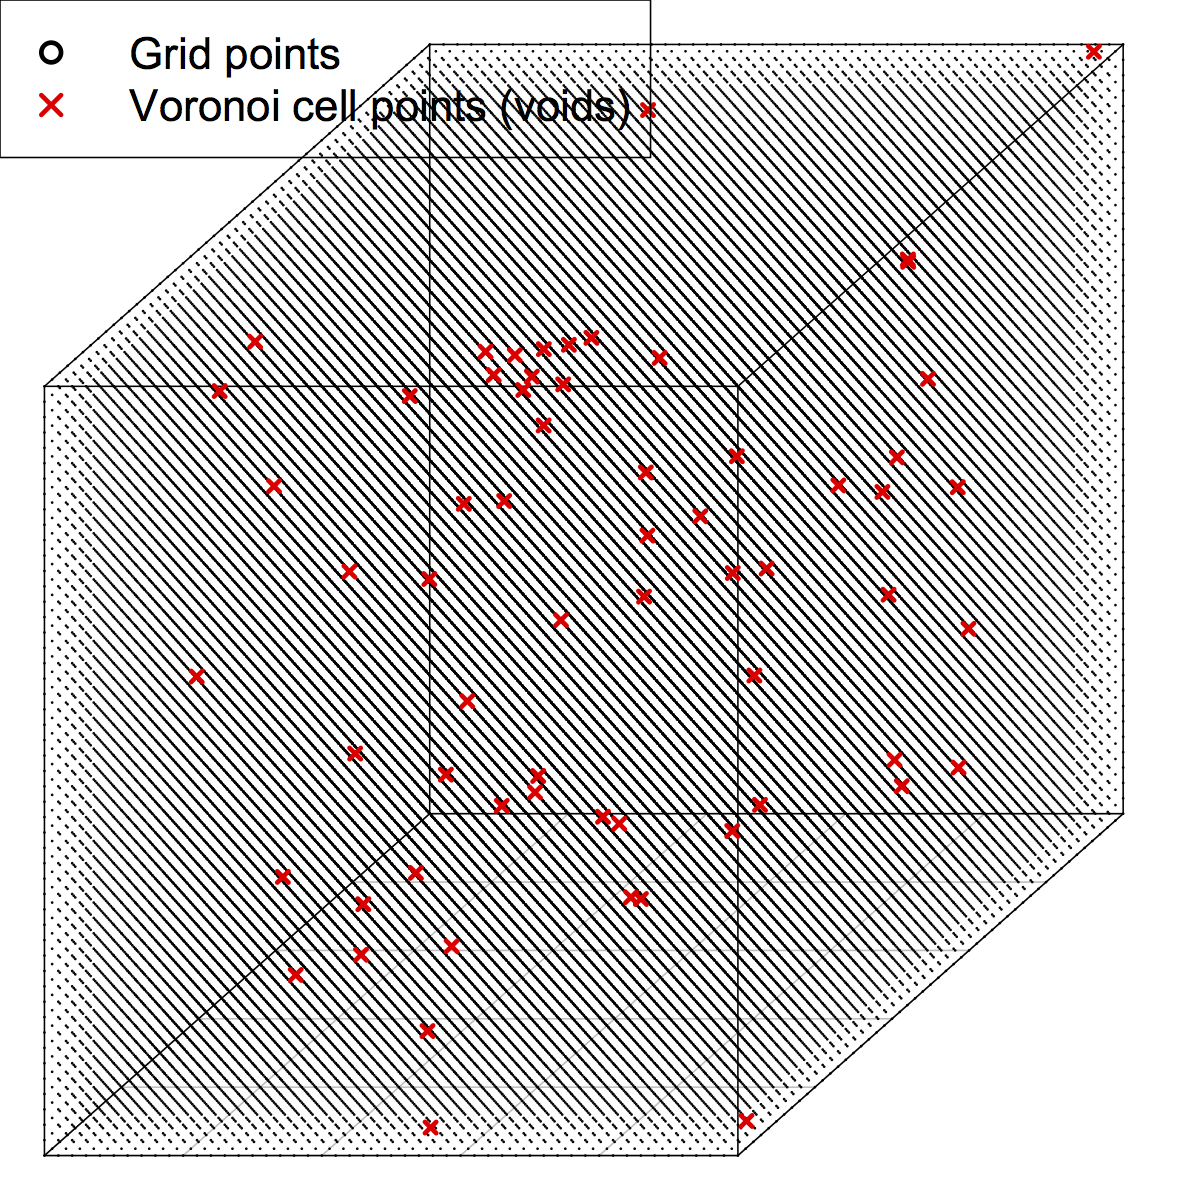
\includegraphics[height=2.25in]{fig_vf_grid.png}
 \label{subfig:grid}
    \end{subfigure}%
    ~
    \begin{subfigure}[t]{0.5\textwidth}
        \centering
                \caption{Cluster points}
        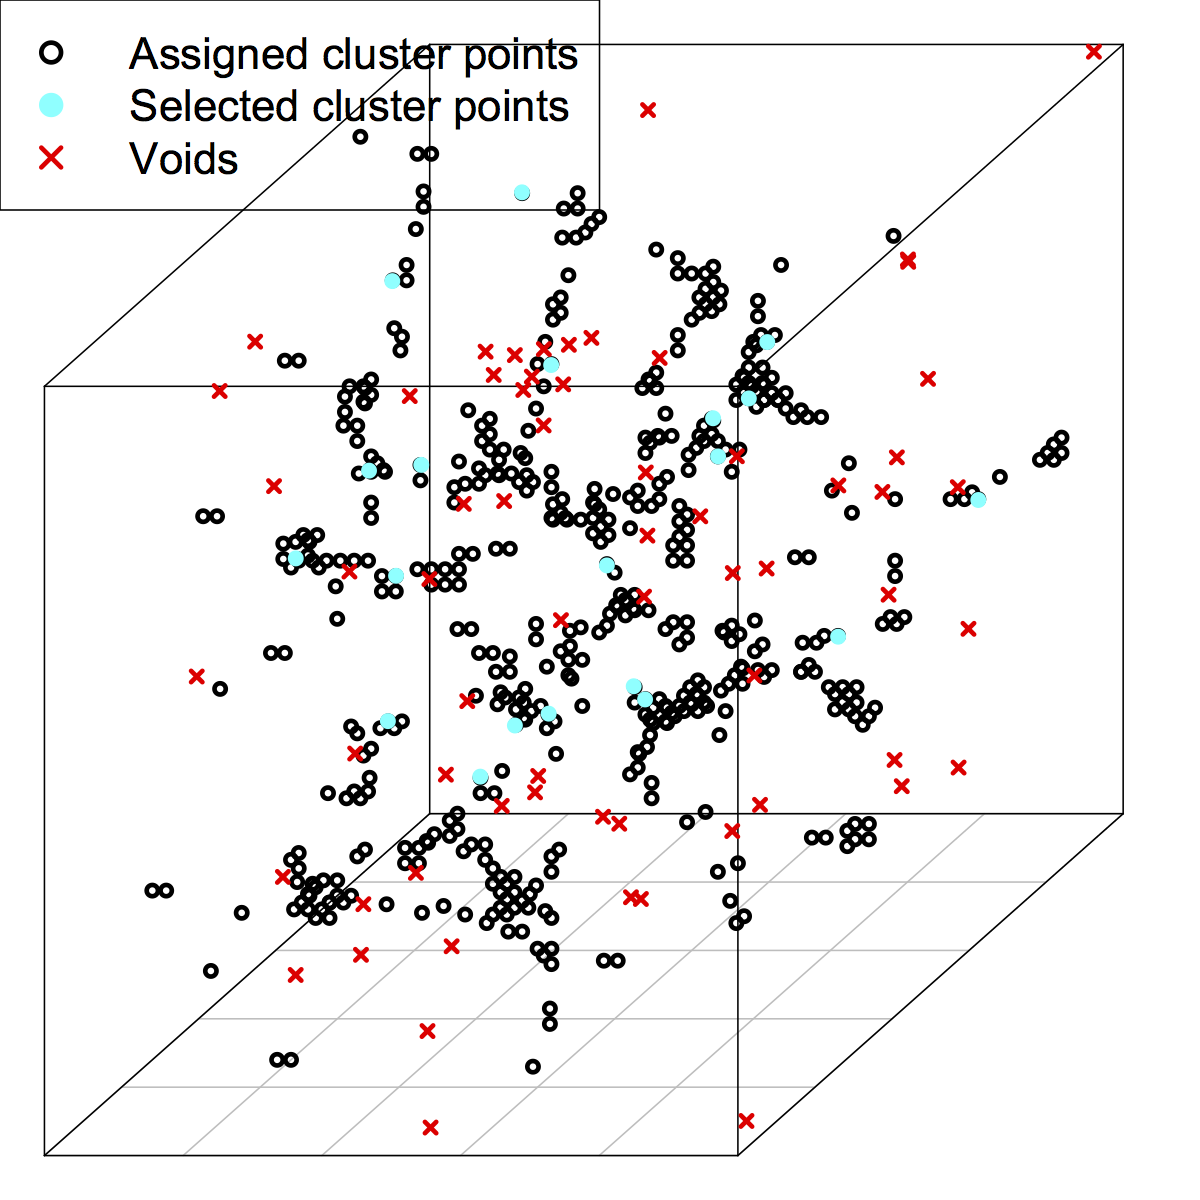
\includegraphics[height=2.25in]{fig_vf_cluster.png}
 \label{subfig:cluster}
    \end{subfigure} \\

     \begin{subfigure}[t]{0.5\textwidth}
      \centering
           \caption{Filament points}
    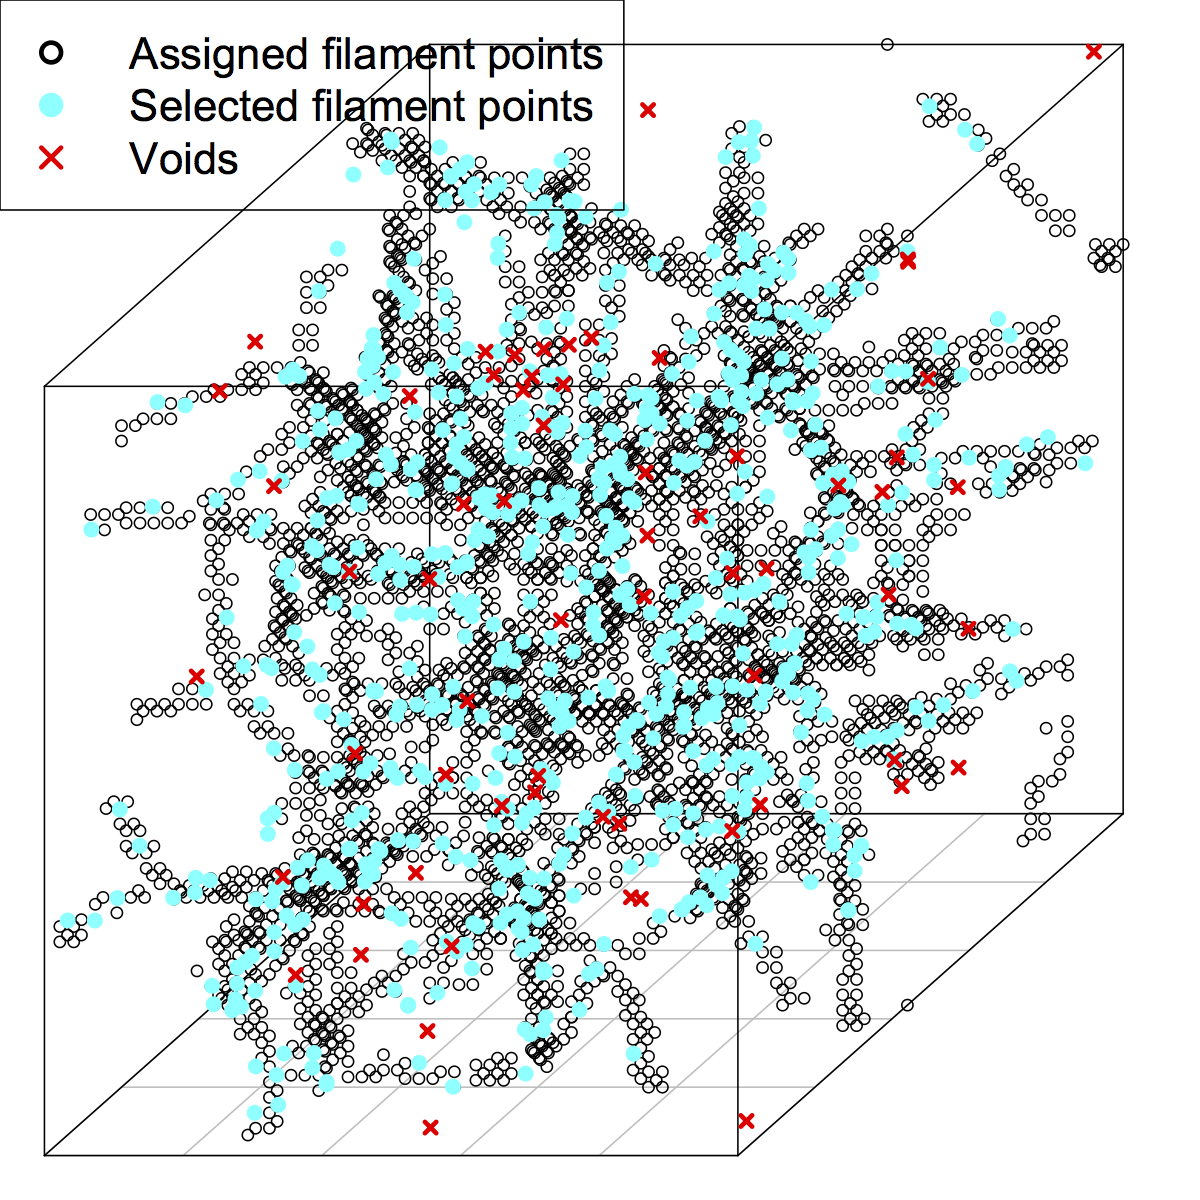
\includegraphics[height=2.25in]{fig_vf_fil.png}
 \label{subfig:fil}
    \end{subfigure}%
    ~
    \begin{subfigure}[t]{0.5\textwidth}
        \centering
                \caption{Wall points}
        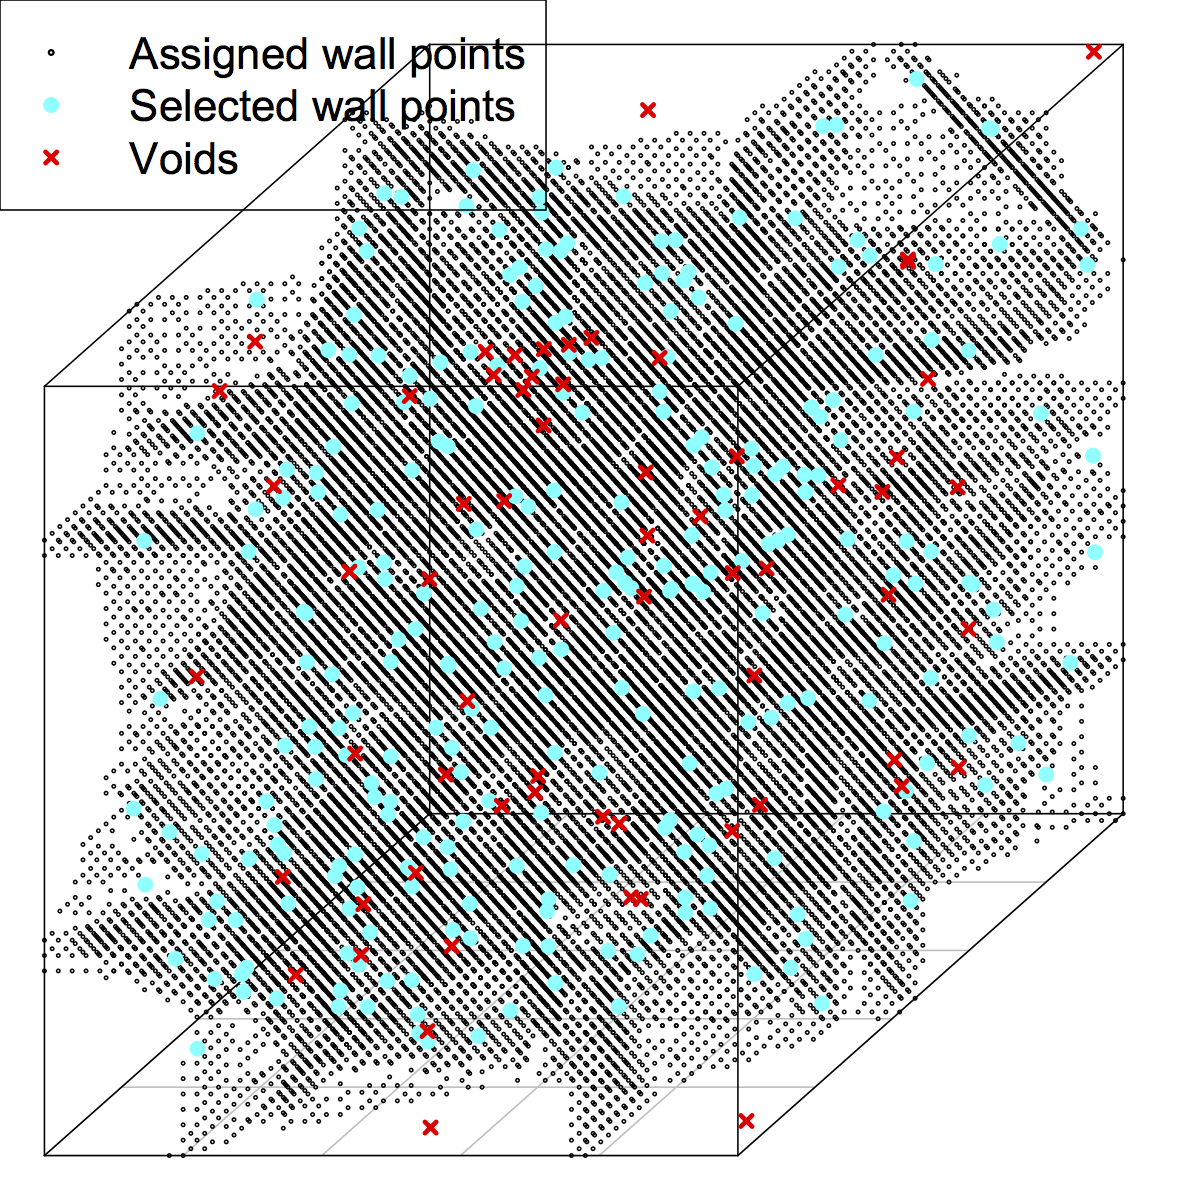
\includegraphics[height=2.25in]{fig_vf_wall.png}
 \label{subfig:wall}
    \end{subfigure}
    \caption{Simulation model construction.  (a) A grid is defined and points are randomly selected to define the Voronoi tesselation - the Voronoi cells are the voids.  (b) - (d) Based on the location of the voids and the grid, points are defined to be cluster points, filament points or wall points - these are the empty black circles.  Based on the values assigned from Table~\ref{table:voronoisettings}, points are randomly selected from the assigned points to be in the final dataset.} \label{fig:vf}
\end{figure*}

% introduced the Voronoi foam as a packing of polyhedral units with walls representing pancakes, edges representing filaments, and vertices representing clusters in the galaxy. Icke showed that the Voronoi foam is an appropriate model for a 10-500 Mpc scale Universe with pressure-free Newtonian gravitational collapse. Statistical study showed that the spatial two-point correlation of Voronoi foams has a power law behavior with close to identical amplitude and slope as that of actual Abell clusters \citep{vanvoronoi}.
% A Voronoi foam model, is generated from a tessellation, where the edges of each cell represent filaments and the faces of the cell, enclosed voids. Given a plane with fixed size, such a tessellation partitions the plane into cellular regions with nuclei. Every cell territory is defined as the set of points equal or closer to that cell's nuclei than any other. To produce a simulation in polynomial time, each point in the plane is compared to the $k$ closest nuclei using a nearest neighbor algorithm where $k$ is chosen to be a small integer. Gaussian noise is added to perturb the plane and inject randomness. Because the nuclei number and the plane size are variable, the points in the simulation representing filaments, clusters, and walls are variable as well. By choosing a reasonable percentage of filaments and related structures, Voronoi simulations are to approximate the topology and LSS of true simulations of the observable Universe. By varying these percentages and repeating simulations, one can quickly generate a large, labeled data sets for hypothesis testing. Our interest primarily was gauging the effect of changing the percent filament in the Voronoi tessellation on the ability of the hypothesis tests to distinguish two foam models sampled from different tessellations.


Examples of three Voronoi Foam models with percFil 10\%and 90\% are shown in \figref{fig:percfilexample} along with their persistence diagrams. One can see that the as the percFil increases, the web-like structure becomes more pronounced, changing the distribution of topological features.
\begin{center}
  \begin{figure}[htp!]
    \centering
    \begin{subfigure}{.24\textwidth}
      \centering
      \caption{PercFil=10\%}
      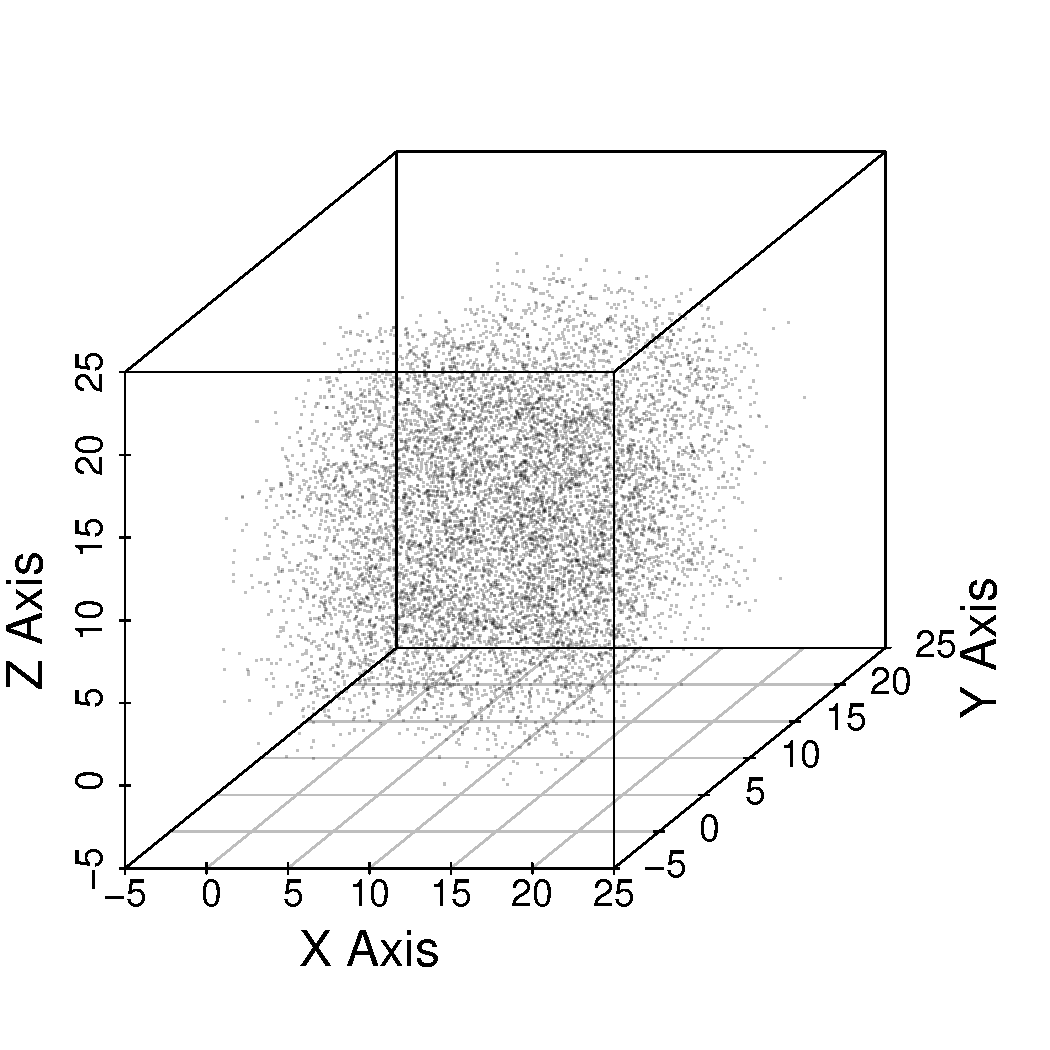
\includegraphics[height=1.5in]{figure_7_plot_pf_0_1.pdf}
      \label{fig:percfil01voronoi}
    \end{subfigure}
    % \begin{subfigure}{.32\textwidth}
    %   \centering
    %   \caption{PercFil = 50\%}
    %   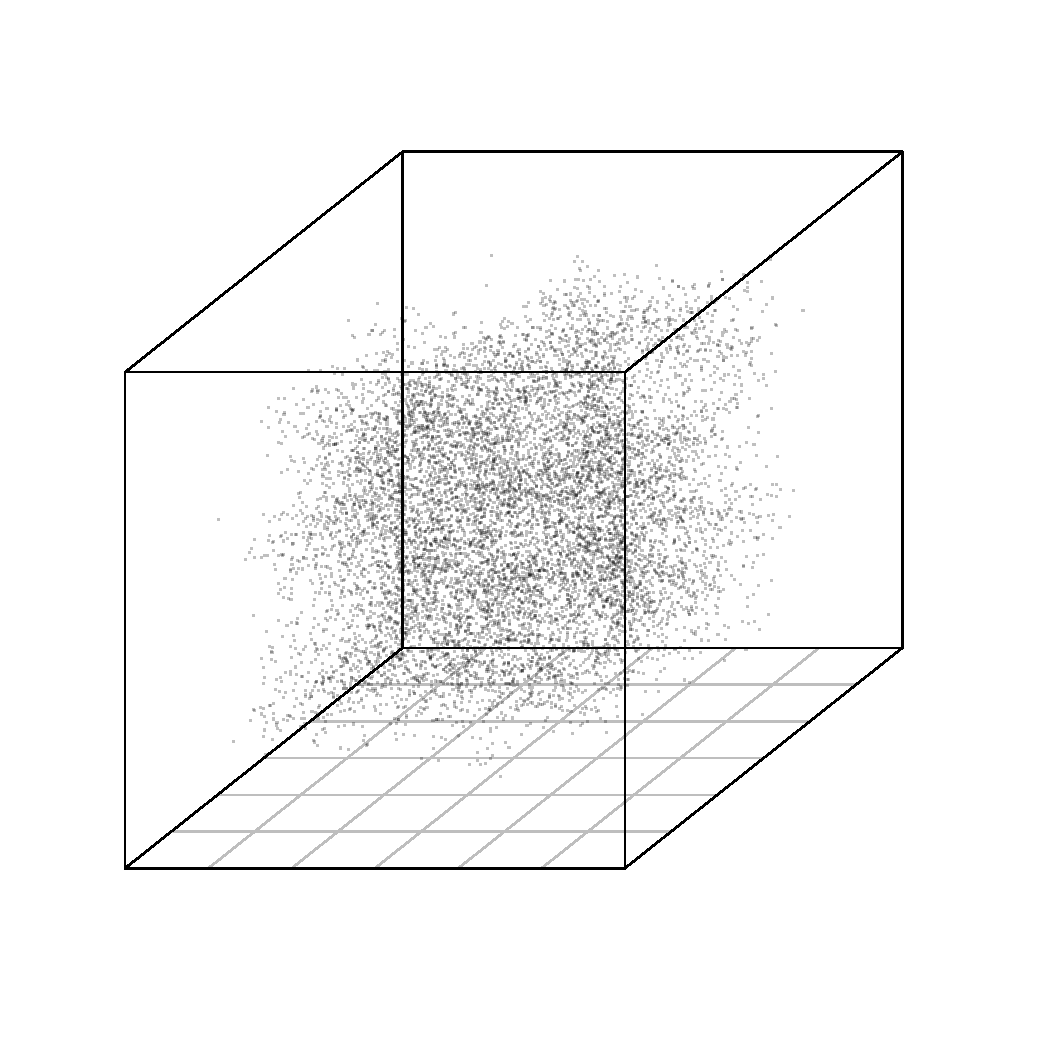
\includegraphics[height=1.5in]{figure_7_plot_pf_0_5.pdf}
    %   \label{fig:percfil09voronoi}
    % \end{subfigure}
    \begin{subfigure}{.24\textwidth}
      \centering
      \caption{PercFil=10\% (PD)}
      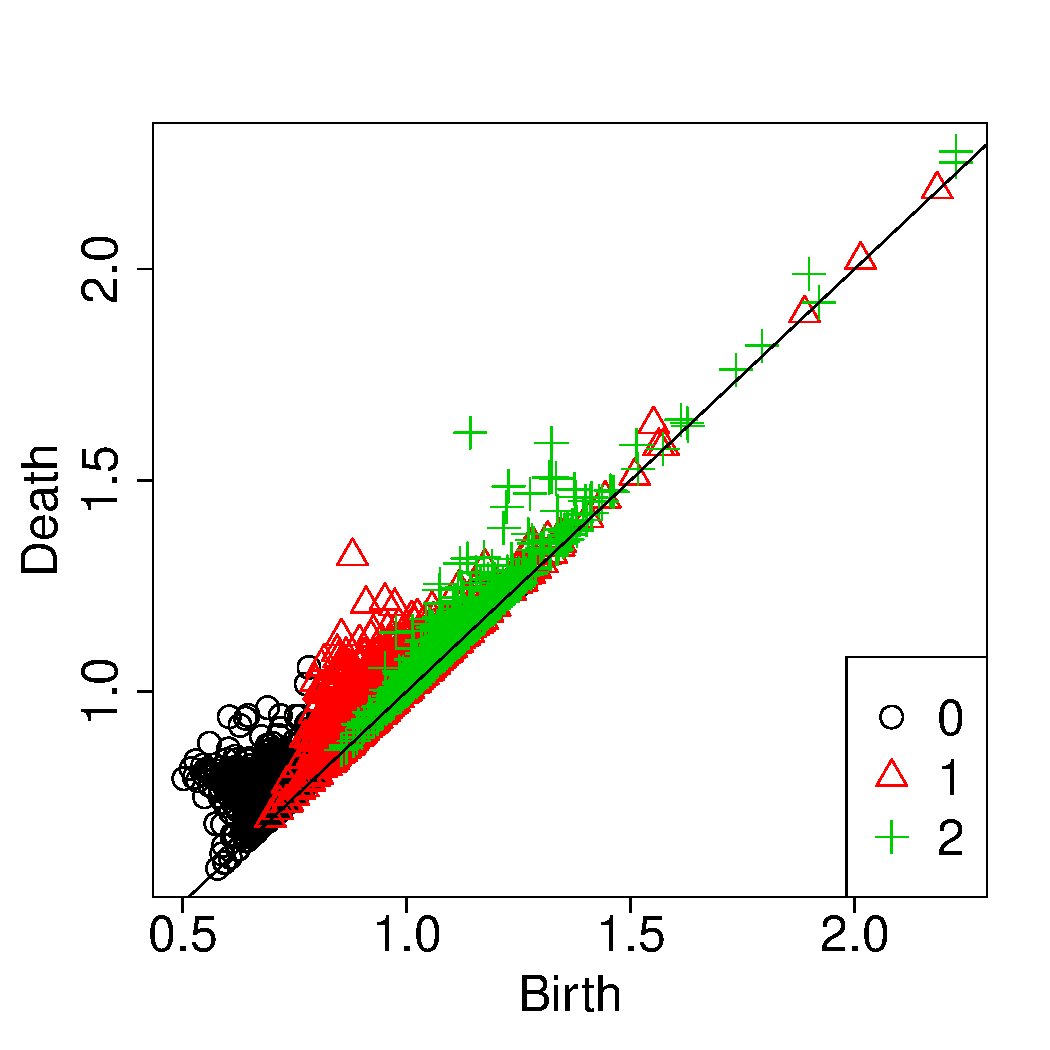
\includegraphics[height=1.5in]{figure_7_pd_0_1.pdf}
      \label{fig:percfil01pd}
    \end{subfigure}
    \begin{subfigure}{.24\textwidth}
      \centering
      \caption{PercFil=90\%}
      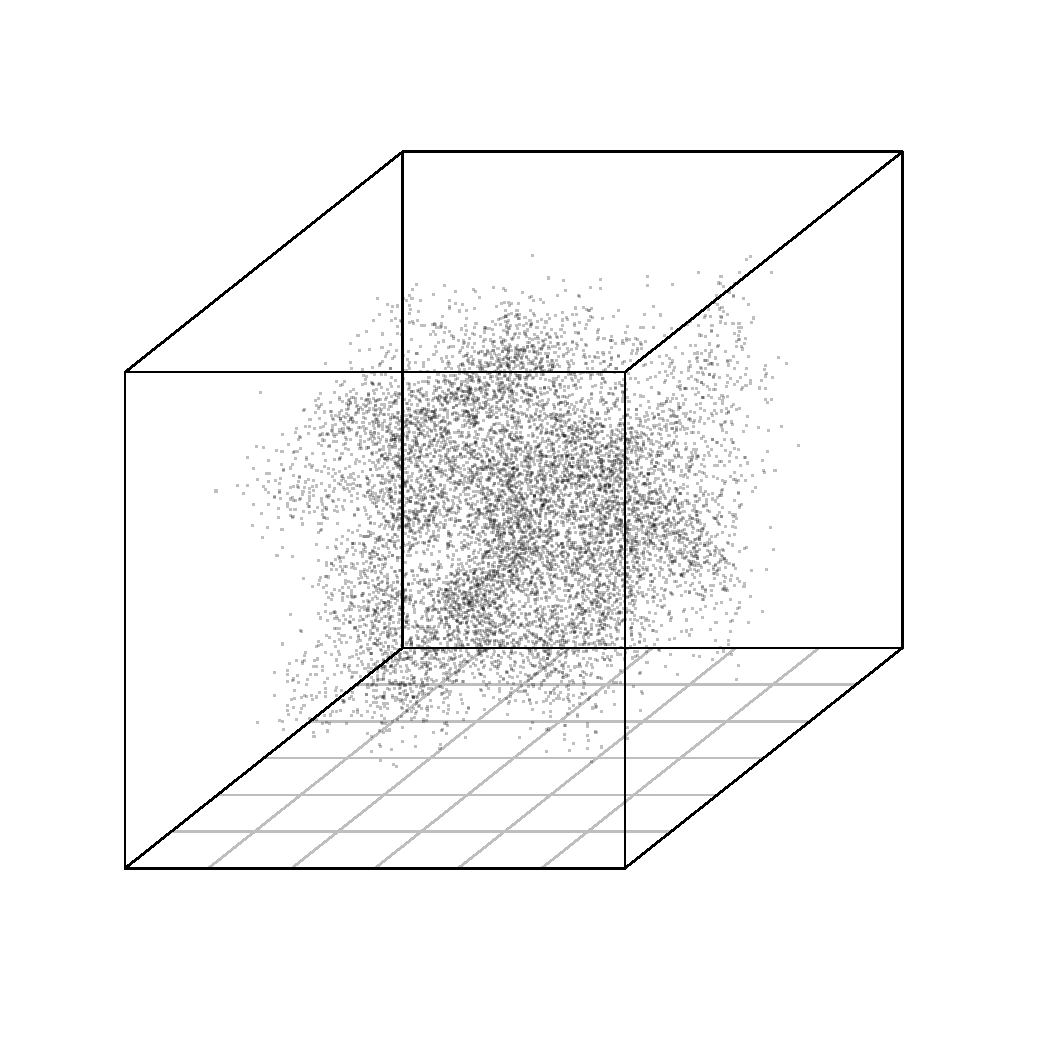
\includegraphics[height=1.5in]{figure_7_plot_pf_0_9.pdf}
      \label{fig:percfil09voronoi}
    \end{subfigure}
    % \begin{subfigure}{.32\textwidth}
    %   \centering
    %   \caption{PercFil = 50\% (PD)}
    %   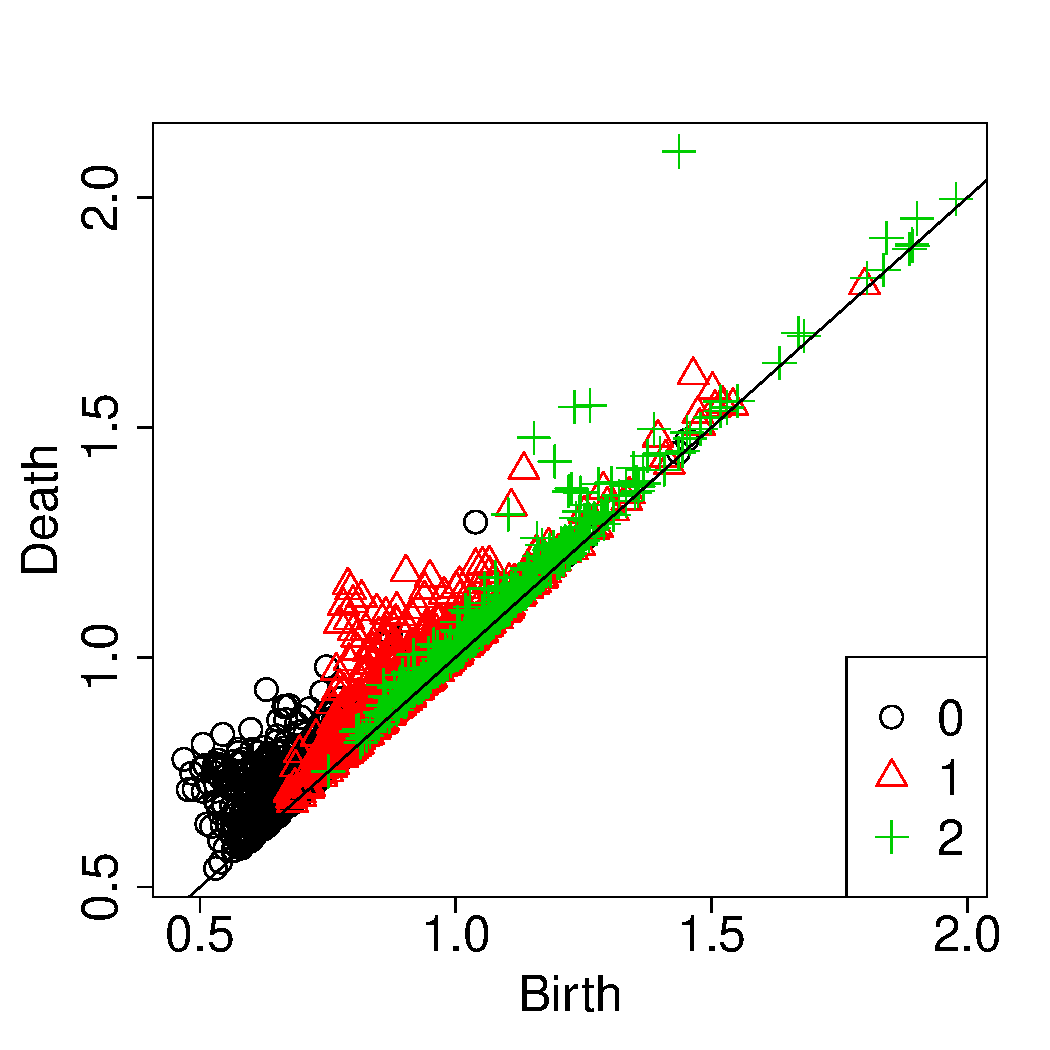
\includegraphics[height=1.5in]{figure_7_pd_0_5.pdf}
    %   \label{fig:percfil09pd}
    % \end{subfigure}
    \begin{subfigure}{.24\textwidth}
      \centering
      \caption{PercFil=90\% (PD)}
      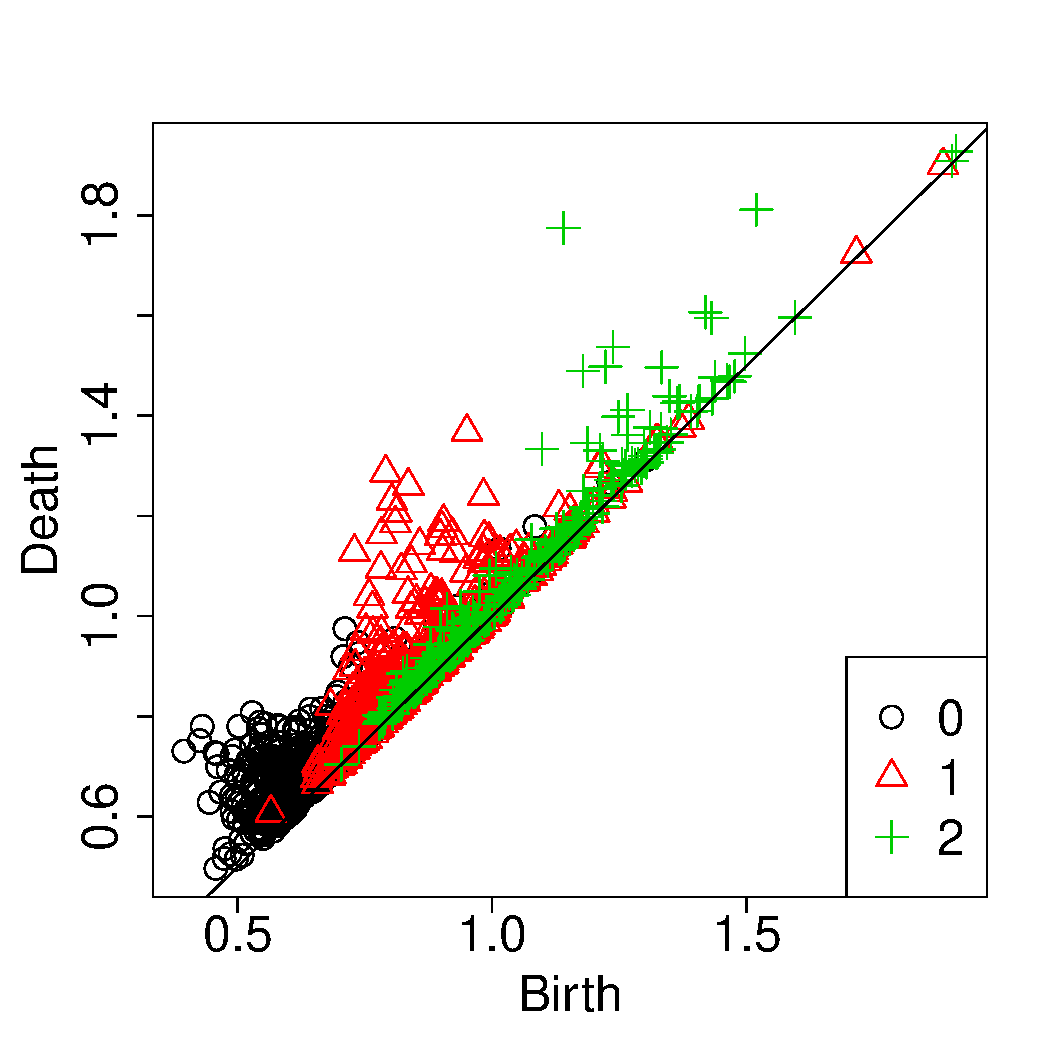
\includegraphics[height=1.5in]{figure_7_pd_0_9.pdf}
      \label{fig:percfil09pd}
    \end{subfigure}
      \caption{Simulated point clouds and their corresponding persistence diagrams (PD) using PercFil of 10\% and 90\%. As the PercFil increases, the point clouds tend to co-agulate into dense and sparse regions; the PDs also form more features with longer lifespans. The other parameters used the generate the data are as defined in Table~\ref{table:voronoisettings}.}
      \label{fig:percfilexample}
  \end{figure}
\end{center}

\subsection{Simulation Study Results}
\label{sec:results1}
The simulated LSS data were generated under $1.25 \times  10^{5}$ box volume, $0.1$ resolution, $1 \times  10^{4}$ points, $64$ cells (voids), percClust = 2\%,  percFil = $[10\%, 30\%]$, and percWall = $[68\%, 88\%]$. 
Persistence diagrams are generated using distance-to-measure (DTM) with a $0.01$ tuning parameter. The diagrams are preprocessed to remove the known 0-dimensional artifact, a vestigial $H_{0}$ element with birth time of 0 and a death time of $\infty$ (with exception to the EC test in which the artifact is preserved). The hypothesis tests were performed on 1000 independent iterations of 15 independent realizations from each of the two populations. The 15 independent datasets are each generated using a percFil setting from 10\% to 30\% (5\% step size).   


Given the data drawn from a model with percFil $p$, each of the proposed test statistics are used to compute a p-value for the test $H_0: \mathcal
P^{(1)} = \mathcal P^{(2)}$ vs. $H_1: \mathcal P^{(1)} \neq \mathcal P^{(2)}$,
based on two samples of persistence diagrams: $\{\mathcal
P_1^{(1)}, \ldots, \mathcal P_{15}^{(1)}\}$ drawn from the model with percFil = 10\%, and $\{\mathcal P_1^{(2)}, \ldots,
\mathcal P_{15}^{(2)}\}$ drawn from the model with percFil = $p$, $p = 10\%, 15\%, \ldots, 30\%$.
(Recall that $\mathcal P^{(1)}$ and $\mathcal P^{(2)}$ are the true underlying distributions of persistence diagrams.)
Similar tests were also completed against a control model with percFil = 30\%, and similar results were found. 


The simulation study results are displayed in \figref{fig:subLinesUnnormApp}, which shows the median $\log_{10}$ p-values along with interval from the $25th$ to the $75th$ quantiles of the 1000 iterations of the proposed test statistics.
We see that  EC,  CORR, and SILEC test are the most effective in distinguishing differences between the models. 
%All other tests are not as sensitive, eventually finding differences between the test and control once percFil approaches 70\% (see Appendix~\ref{app:simulation}). 
Additionally, all tests derived from Euler characteristic functions perform relatively well compared to the other tests, suggesting that the Betti numbers, by being topologically invariant, are much better functional summaries of the persistence diagrams than intensity functions, silhouettes, and landscapes. More interestingly, it is possible that the alternating linear function by which the Betti numbers are combined may better preserve topological information given than the SILEC test, which combines silhouettes through a similar linear fashion, performed better than any individual silhouette counterpart and the naive cross-dimension statistic (SIL$_{0:2}$). Finally,  CORR, though not as powerful as EC, performs well as percFil increases.

% --------------- BEGIN FIGURES -----------------

\begin{center}
  \begin{figure}[htp!]
    \centering
    \begin{subfigure}{.47\textwidth}
      \centering
      \caption{EC Tests}
      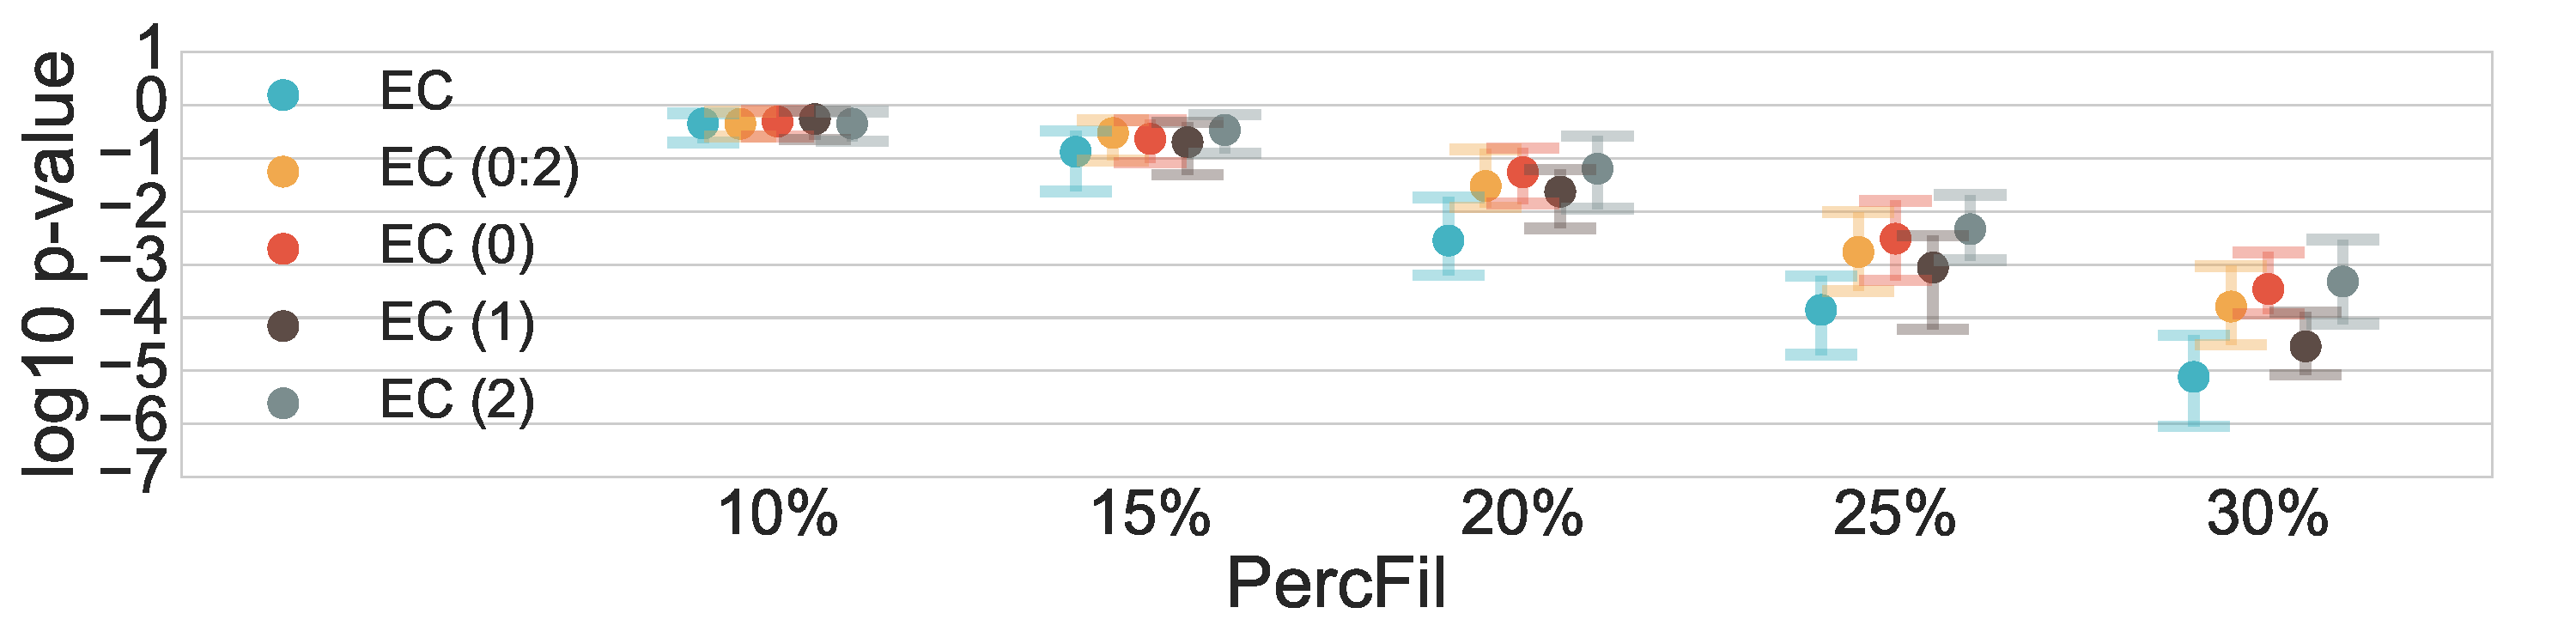
\includegraphics[height = .78in]{figure_8_euler_group.pdf} 
      \label{fig:sub_euler}
    \end{subfigure}
%    \begin{subfigure}{.48\textwidth}
%      \centering
%      \caption{EC Tests (Standardized Ratio)}
%      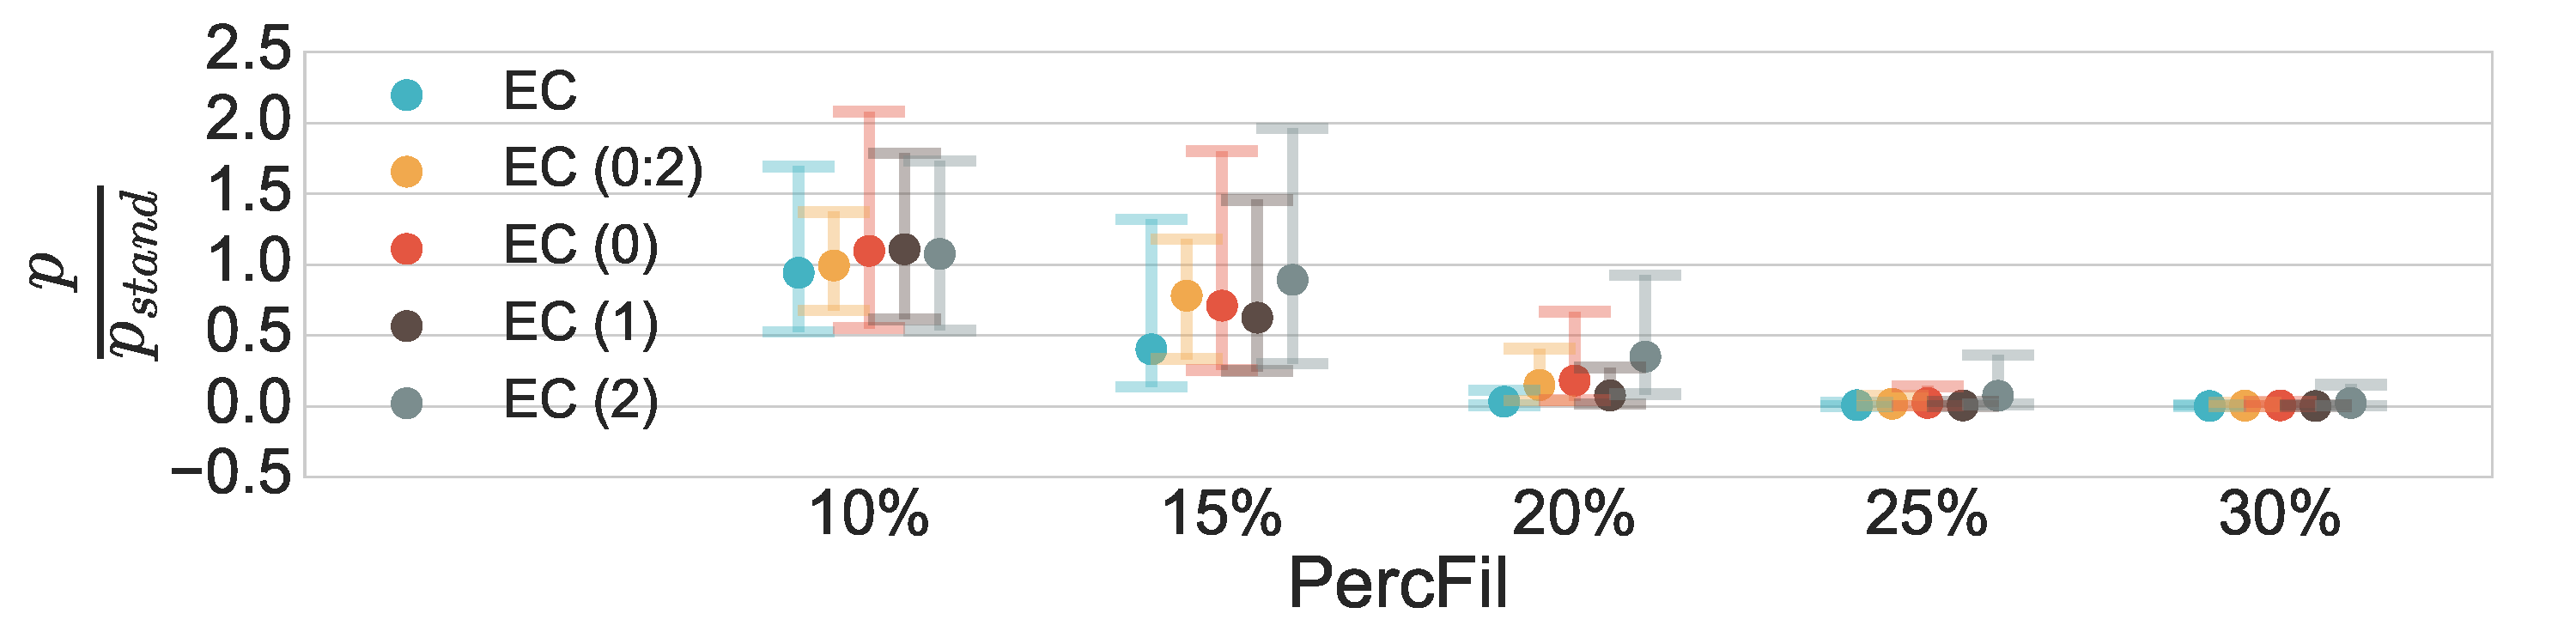
\includegraphics[width=\linewidth, height = .75in]{figure_8_joint_euler_group.pdf}
%      \label{fig:sub_euler_normed}
%    \end{subfigure}
    \begin{subfigure}{.47\textwidth}
      \centering
      \caption{SIL Tests}
      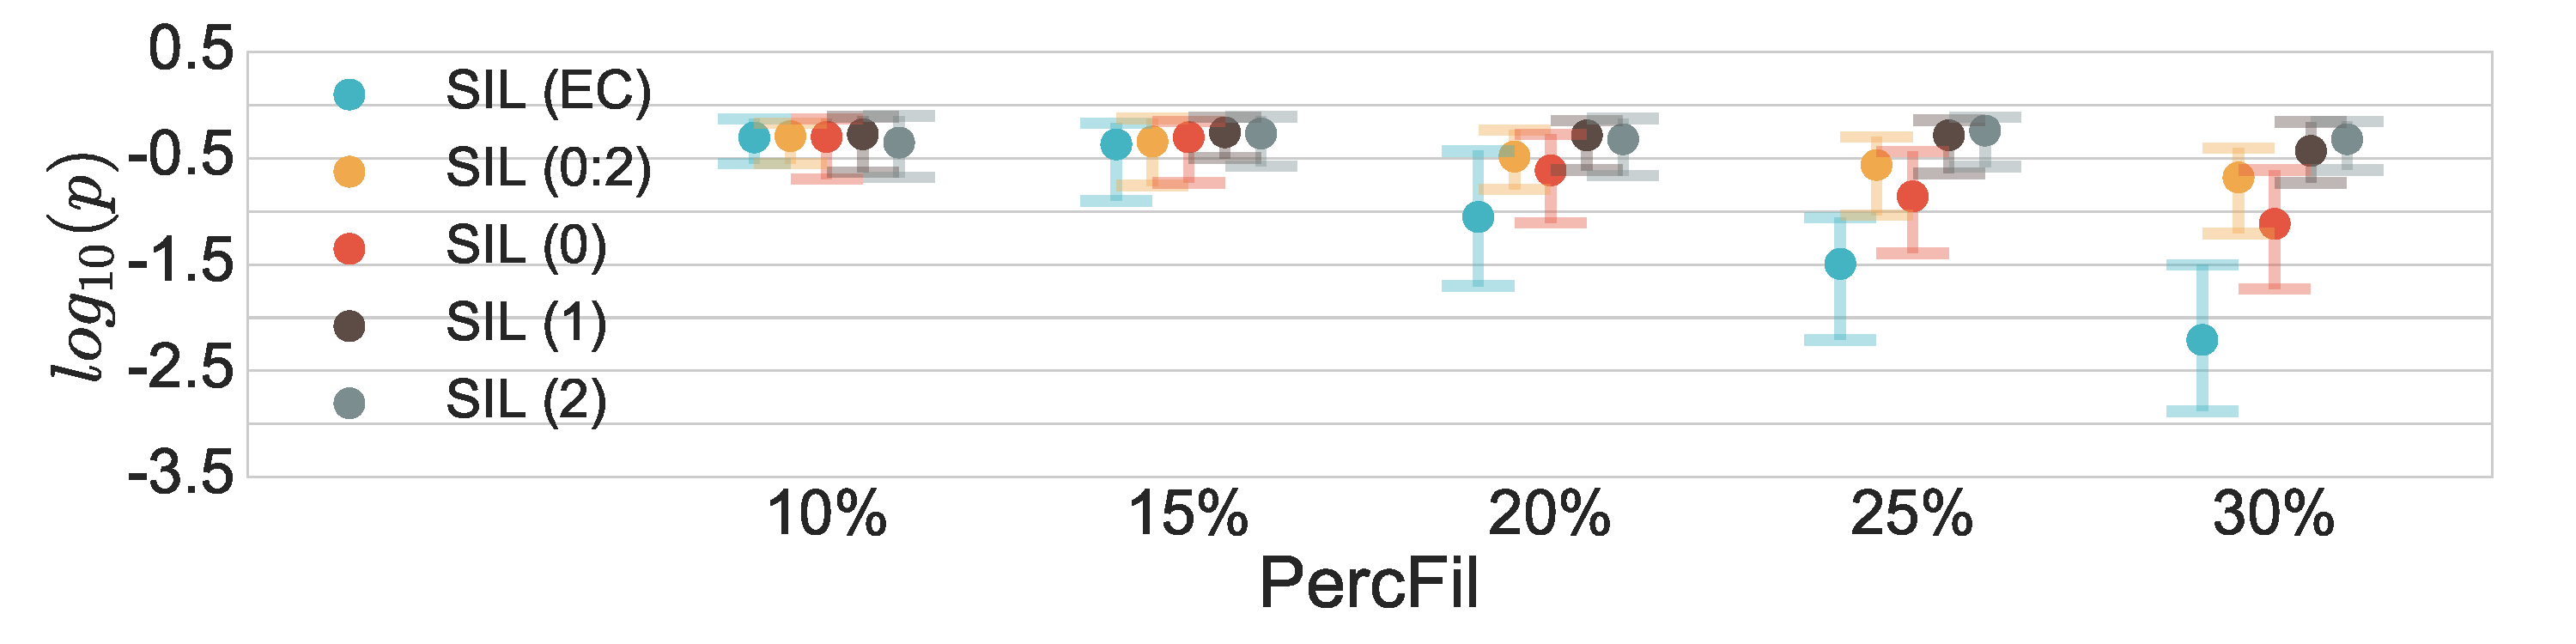
\includegraphics[height = .78in]{figure_8_silhouette_group.pdf}
      \label{fig:sub_silh}
    \end{subfigure}
%    \begin{subfigure}{.48\textwidth}
%      \centering
%      \caption{SIL Tests (Standardized Ratio)}
%      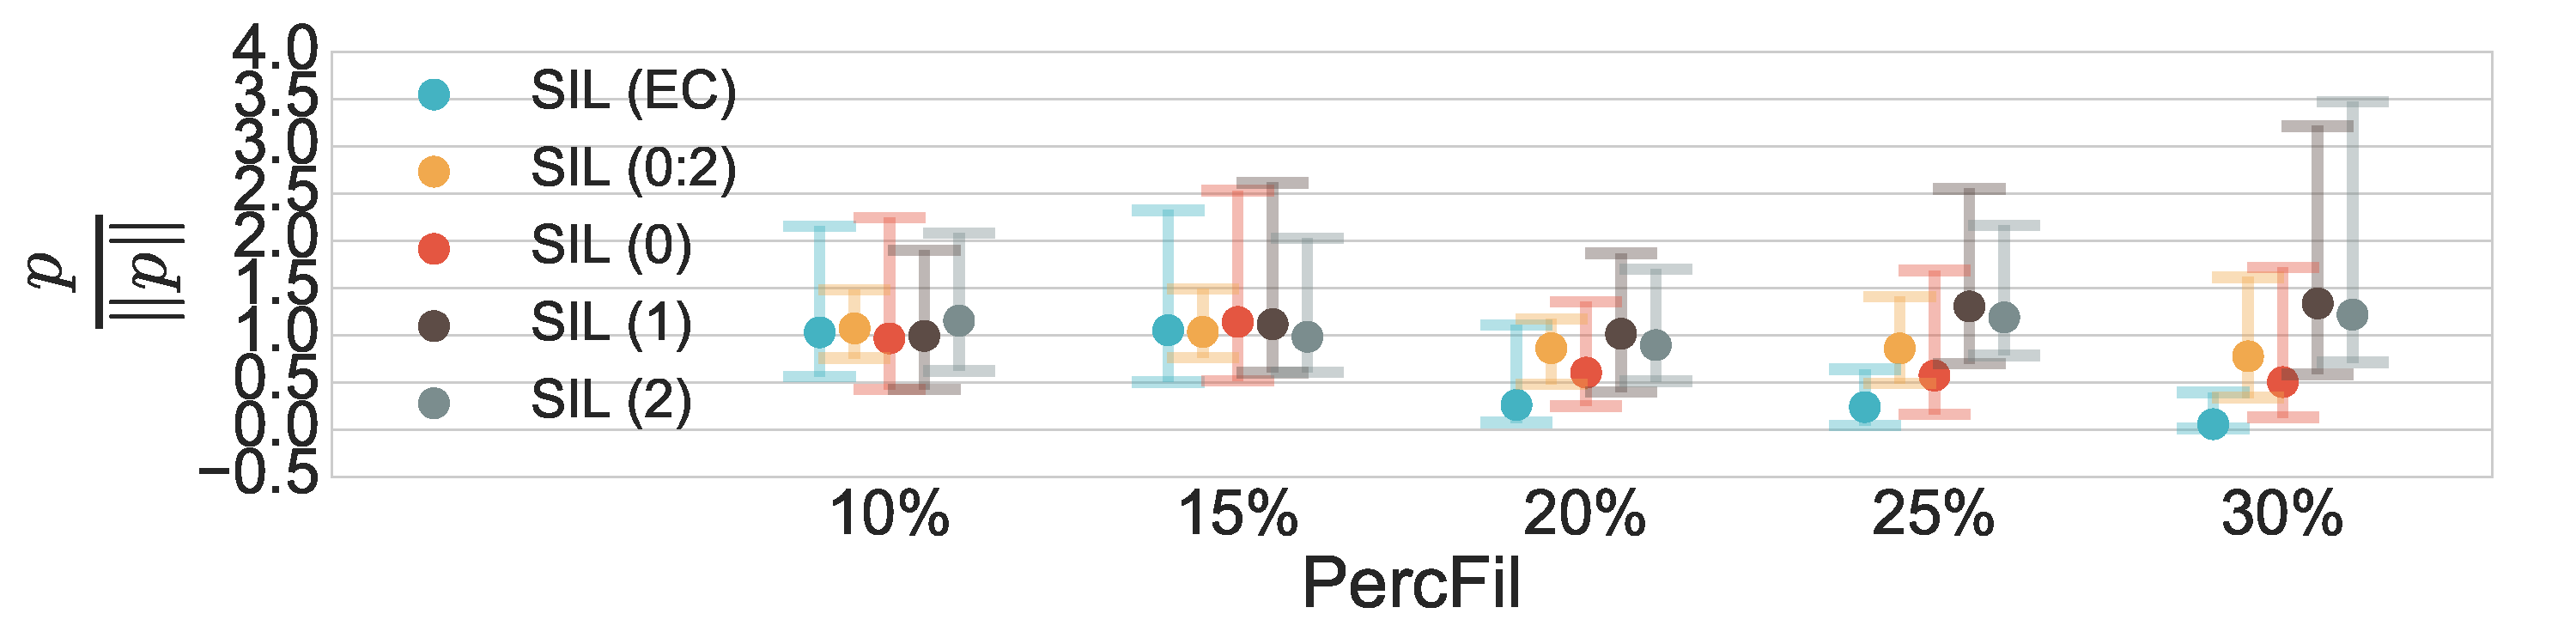
\includegraphics[width=\linewidth, height = .75in]{figure_8_joint_silhouette_group.pdf}
%      \label{fig:sub_silh_normed_normed}
%    \end{subfigure}
    \begin{subfigure}{.47\textwidth}
      \centering
      \caption{IK Tests}
      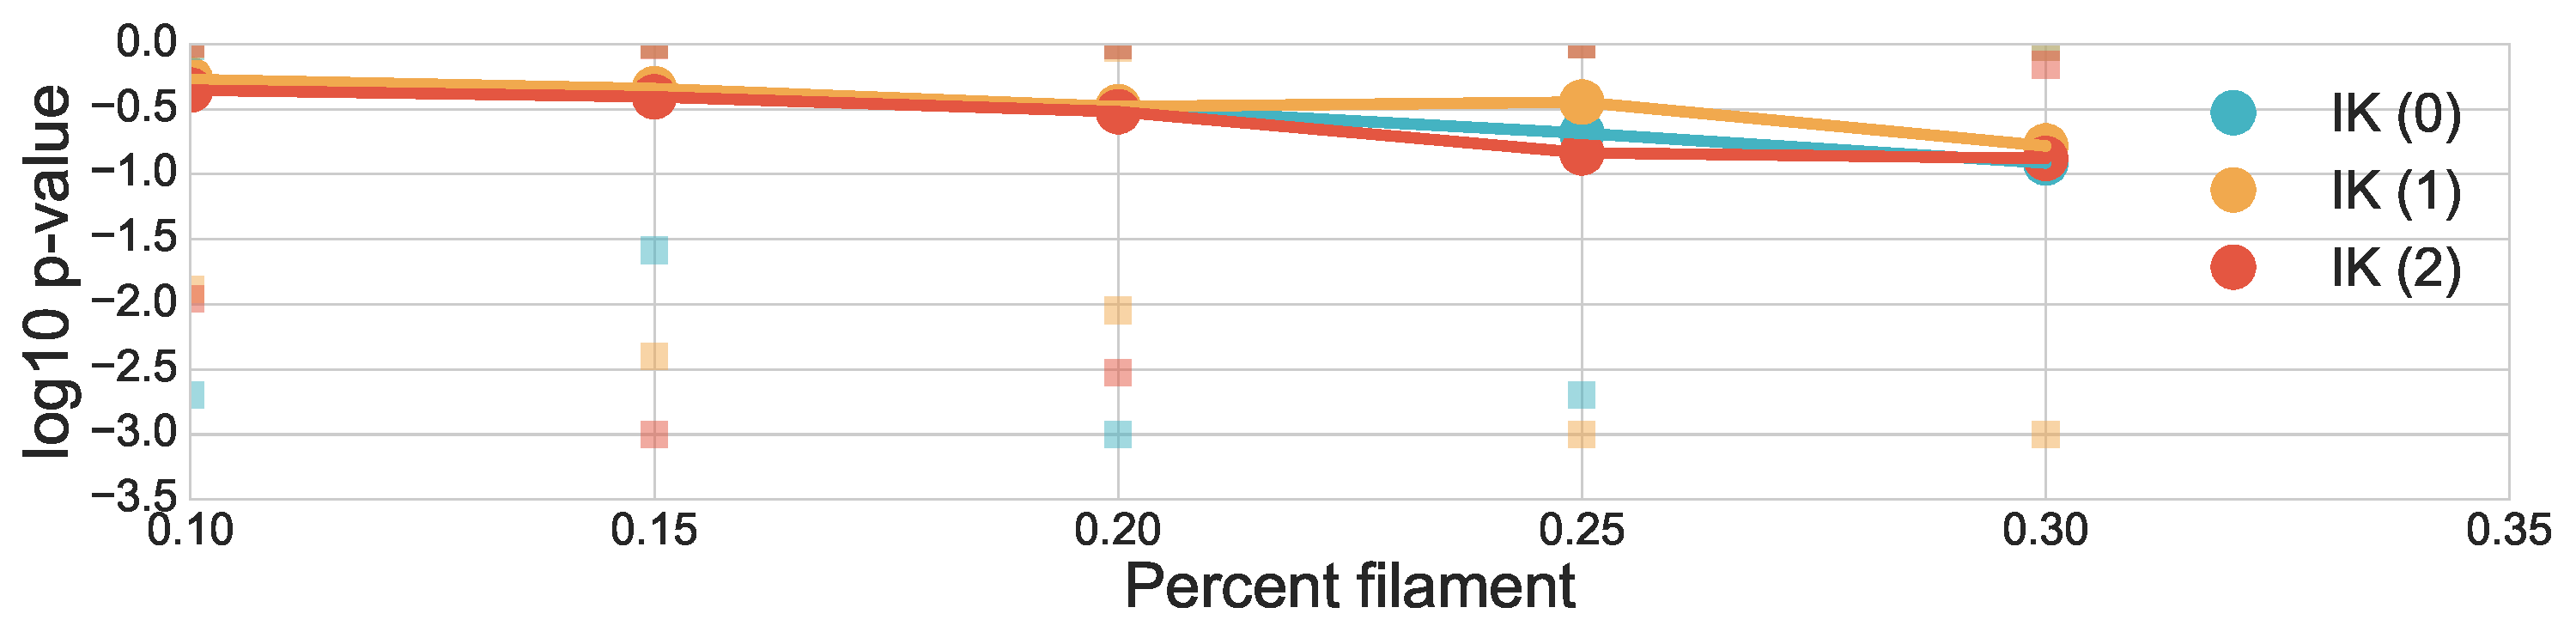
\includegraphics[height = .78in]{figure_8_contour_group.pdf}
      \label{fig:sub_contour}
    \end{subfigure}
%    \begin{subfigure}{.48\textwidth}
%      \centering
%      \caption{IK Tests (Standardized Ratio)}
%      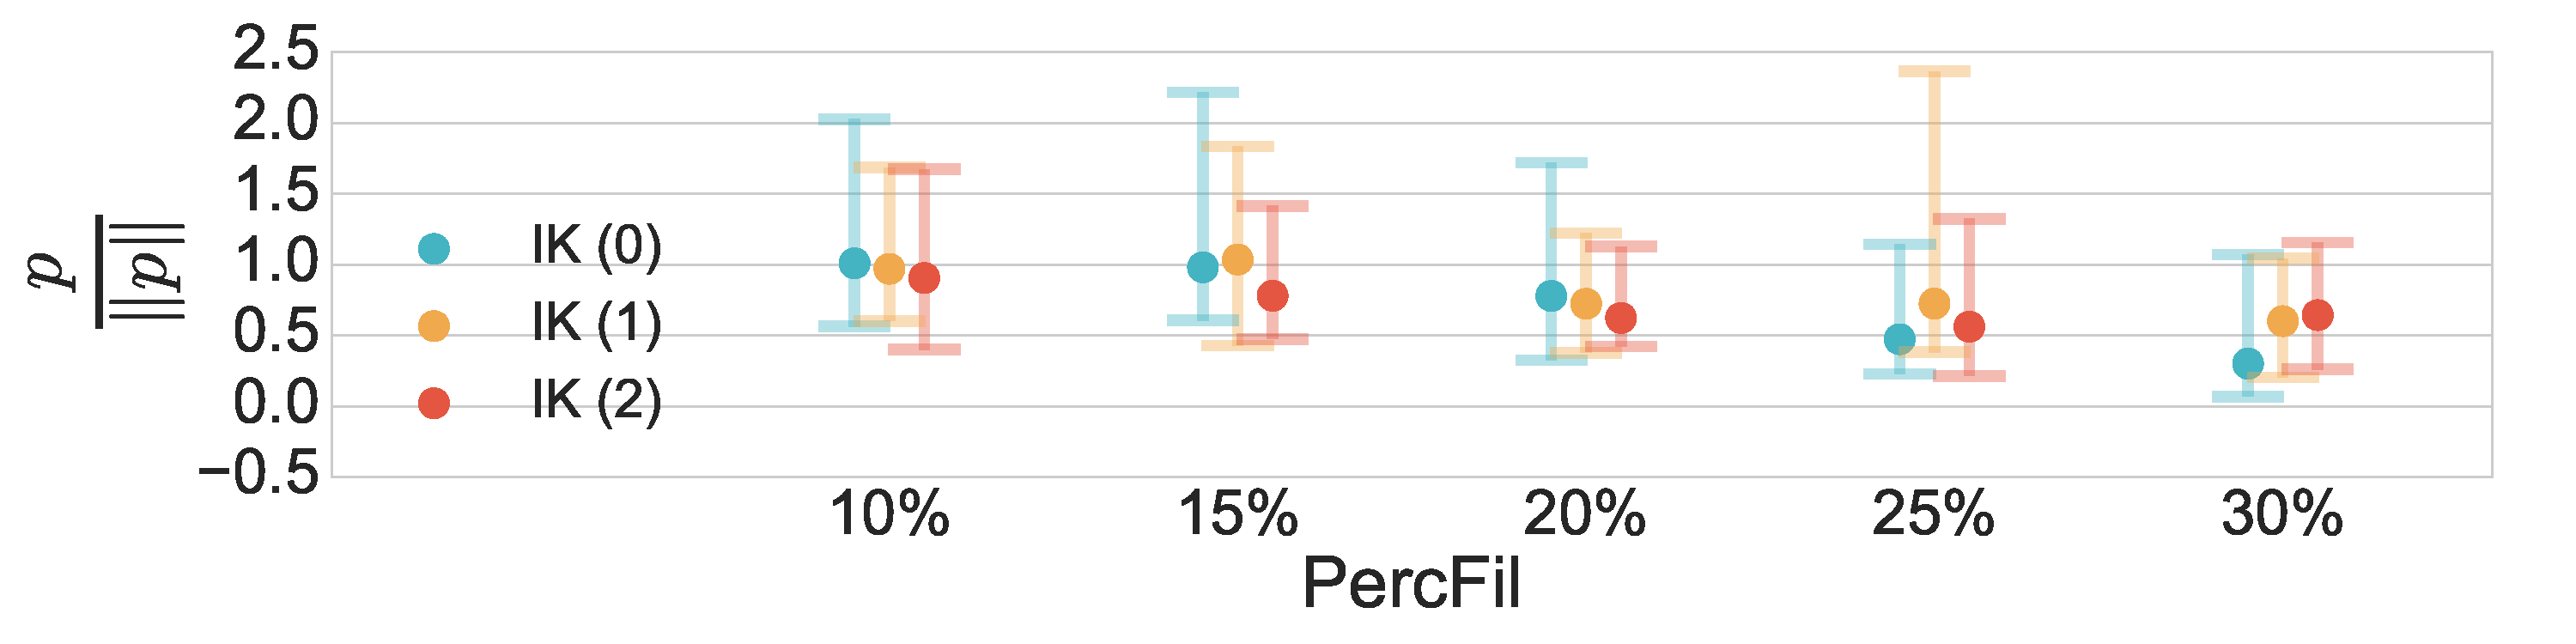
\includegraphics[width=\linewidth, height = .75in]{figure_8_joint_contour_group.pdf}
%      \label{fig:sub_contour_normed}
%    \end{subfigure}
    \begin{subfigure}{.47\textwidth}
      \centering
      \caption{WIK/PI Tests}
      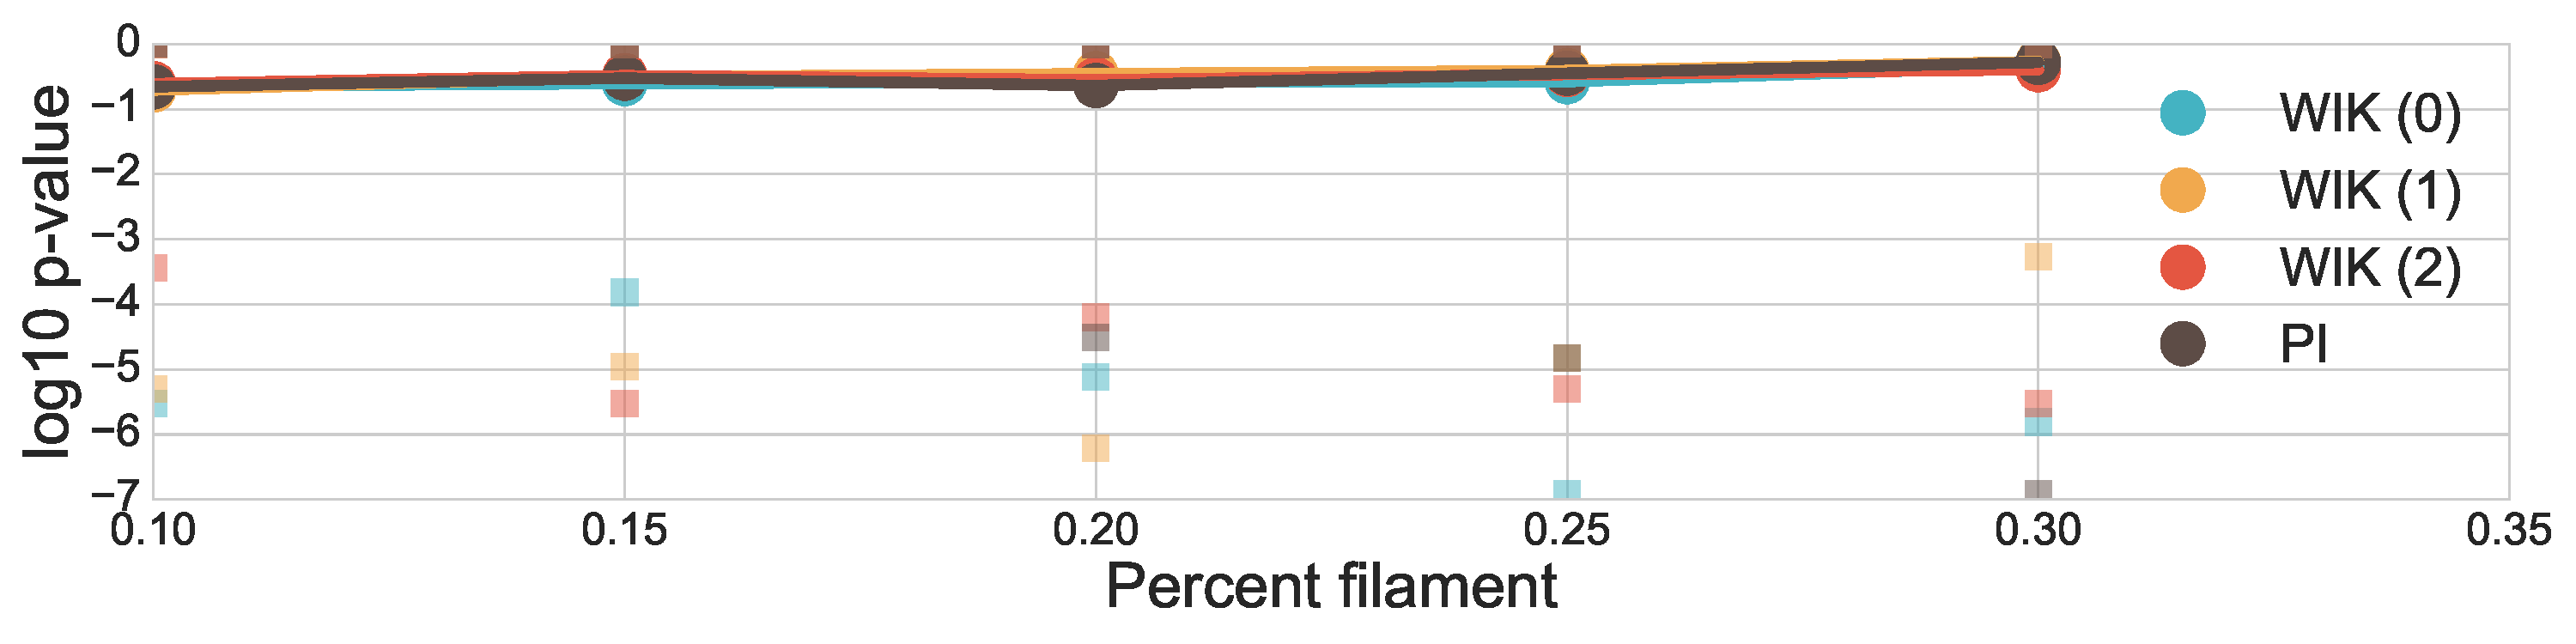
\includegraphics[height = .78in]{figure_8_weighted_contour_group.pdf}
      \label{fig:sub_weight}
    \end{subfigure}
%    \begin{subfigure}{.48\textwidth}
%      \centering
%      \caption{WIK/PI Tests (Standardized Ratio)}
%      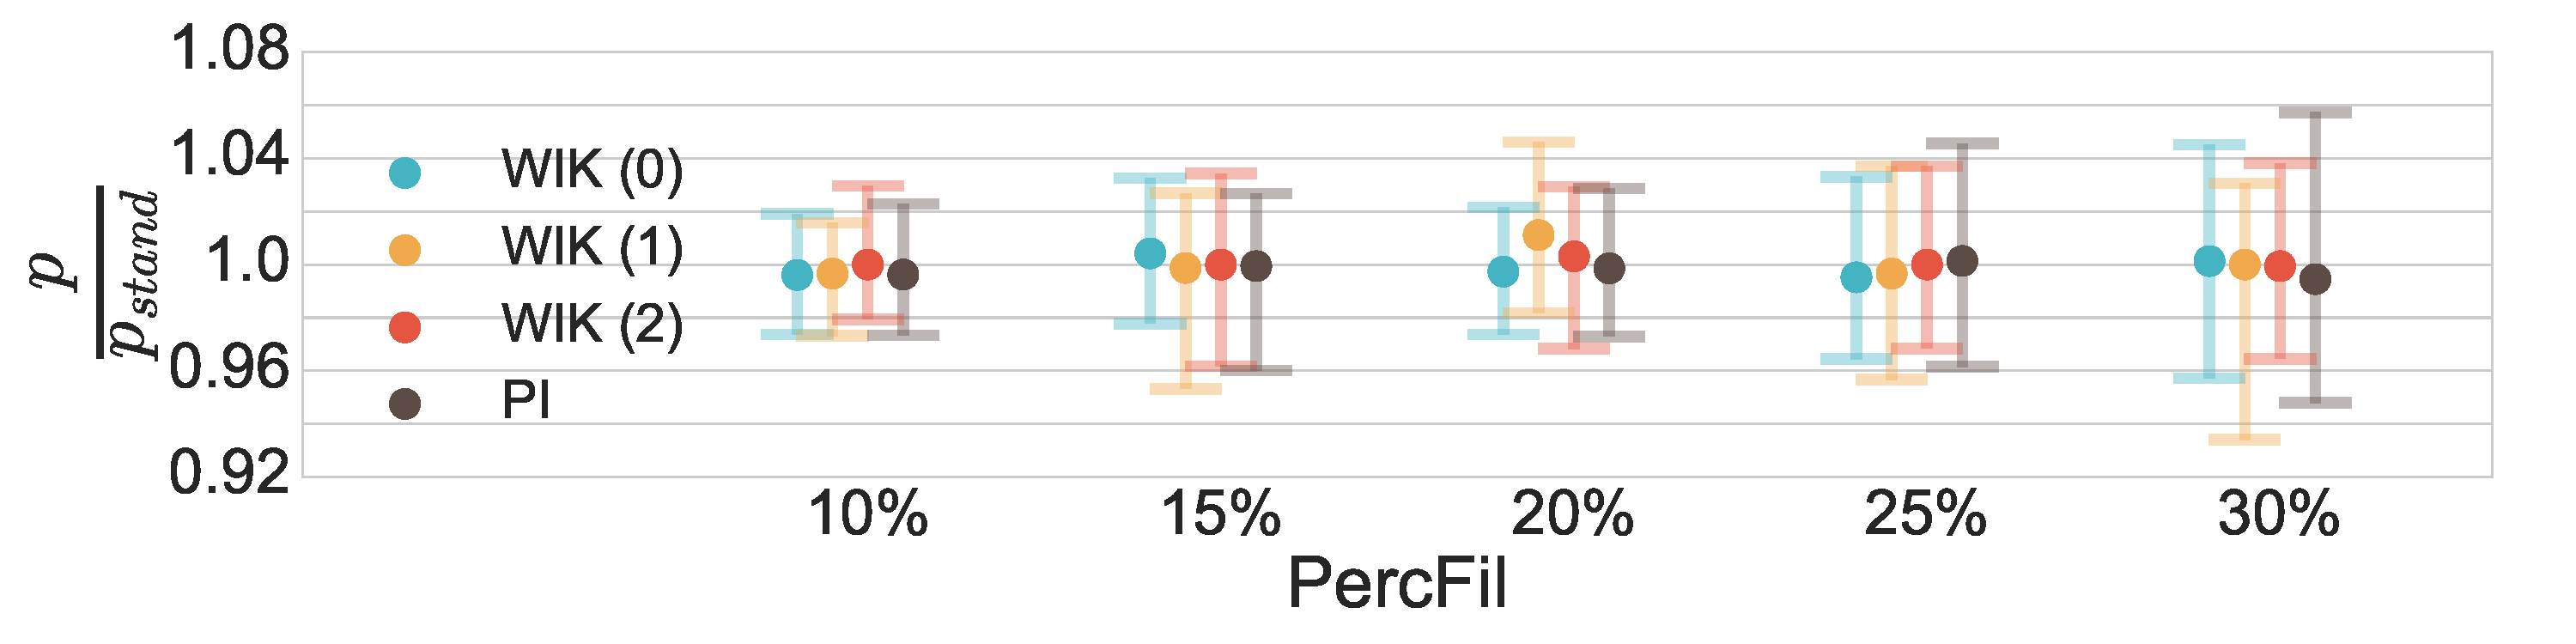
\includegraphics[width=\linewidth, height = .75in]{figure_8_joint_weighted_contour_group.pdf}
%      \label{fig:sub_weight_normed}
%    \end{subfigure}
    \begin{subfigure}{.47\textwidth}
      \caption{CORR Tests}
      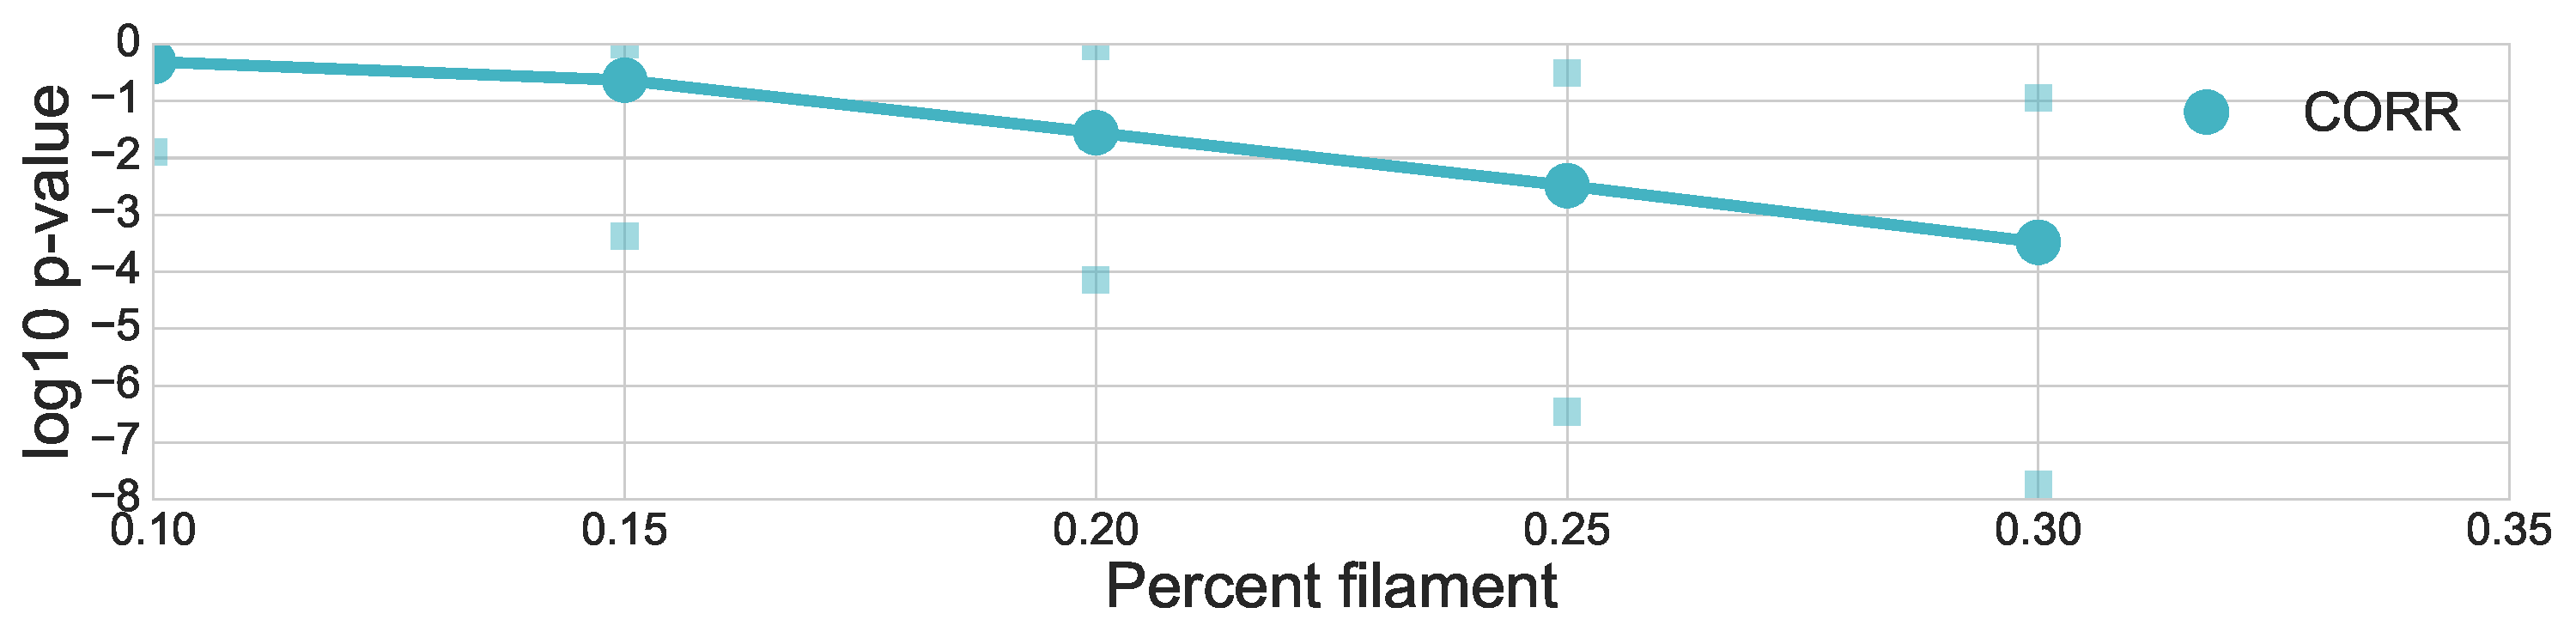
\includegraphics[height = .78in]{figure_8_correlation_group.pdf}
      \label{fig:sub_corr}
    \end{subfigure}
%    \begin{subfigure}{.48\textwidth}
%      \caption{CORR Tests (Standardized Ratio)}
%      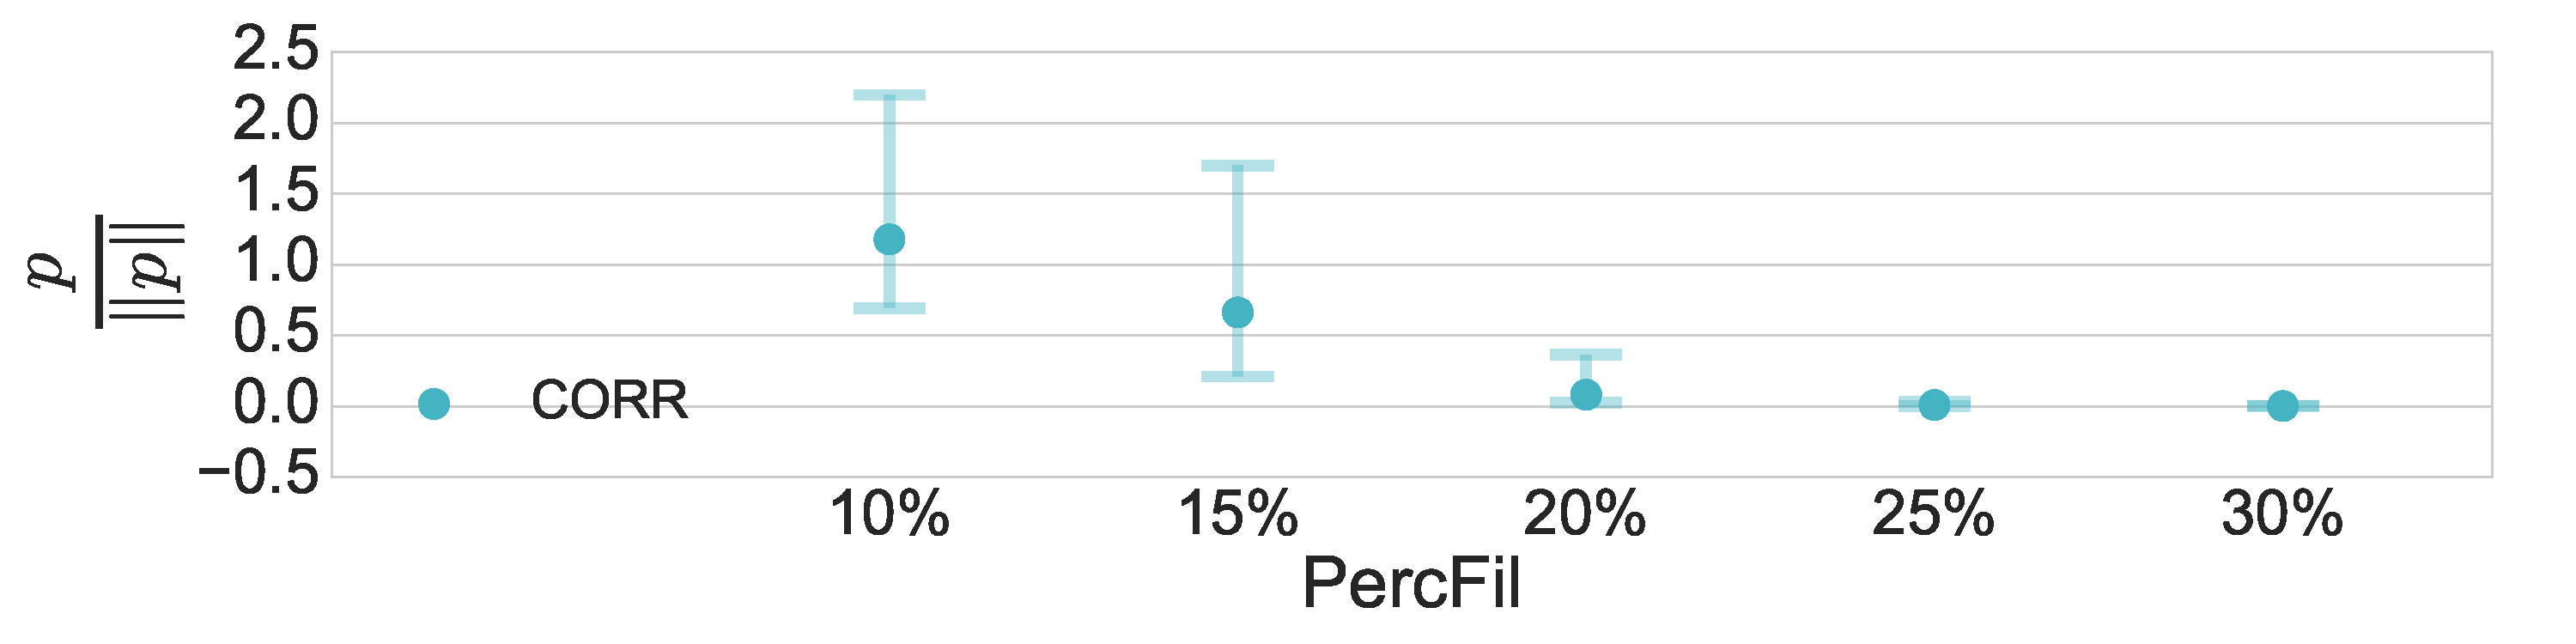
\includegraphics[width=\linewidth, height = .75in]{figure_8_joint_correlation_group.pdf}
%      \label{fig:sub_corr_normed}
%    \end{subfigure}
    \begin{subfigure}{.47\textwidth}
      \caption{Comparison of Tests}
      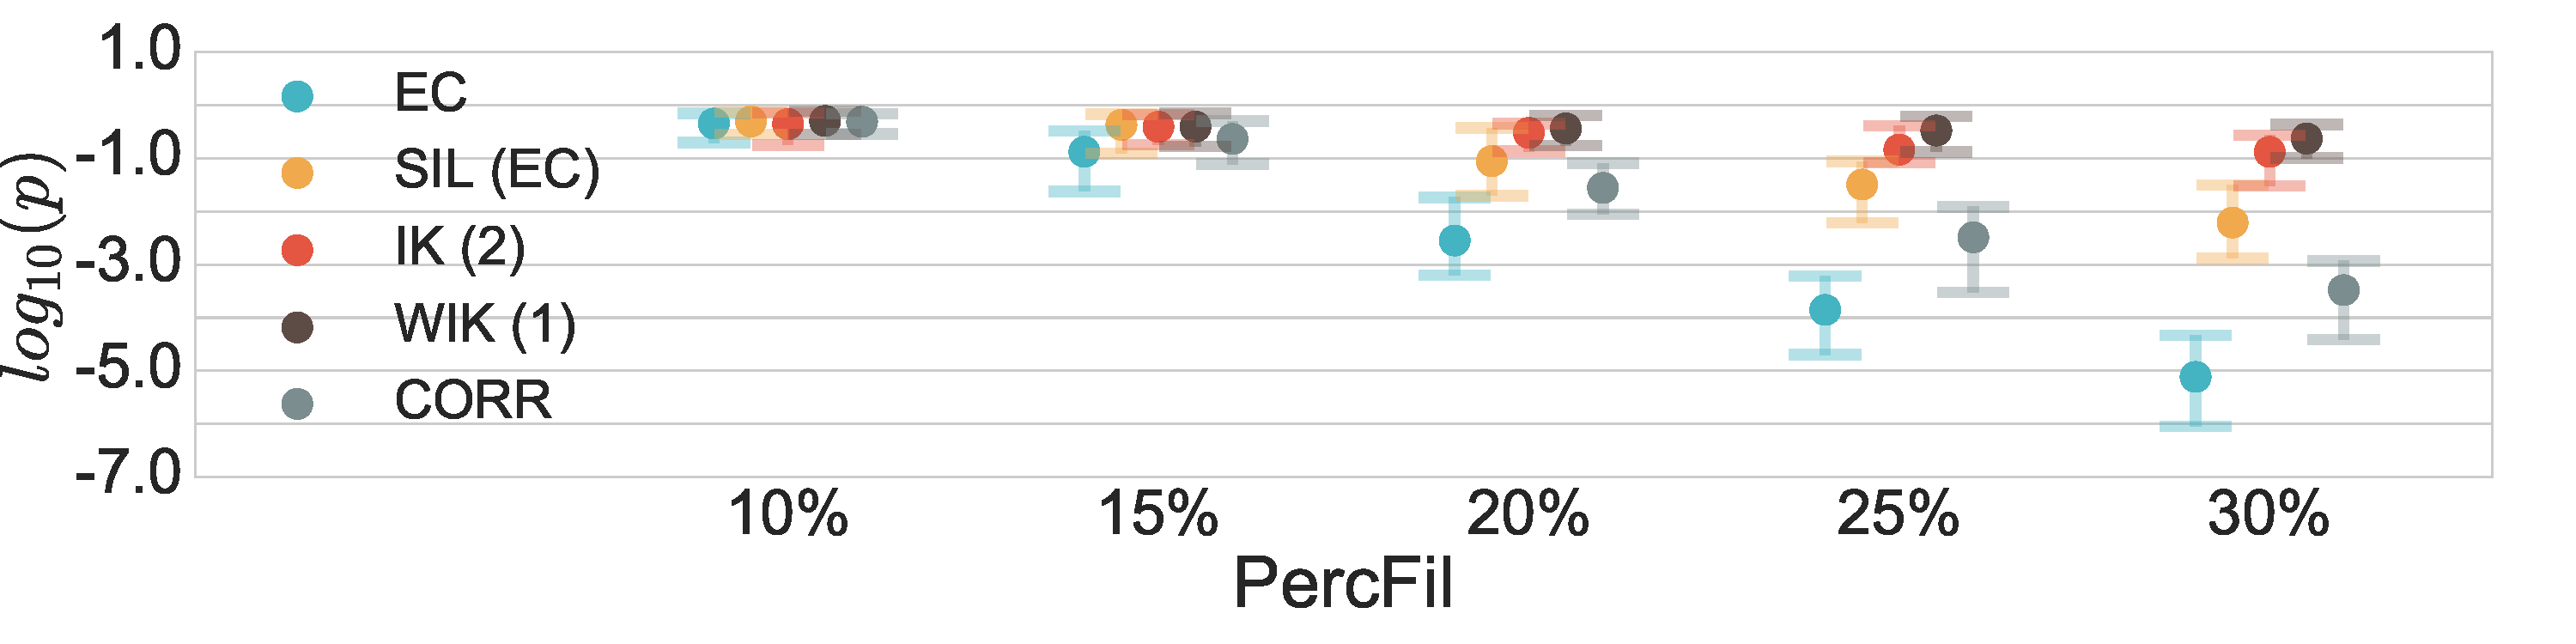
\includegraphics[height = .78in]{figure_8_best_group}
      \label{fig:sub_best}
    \end{subfigure}
    \caption{Results for EC, SIL, IK, WIK/PI, and CORR tests. X-axis represents the true PercFil (10\%, 15\%, 20\%, 25\%, 30\%), compared to the null PercFil of 10\%; The vertical axis shows the $\log_{10}$(p-values). The lines plots the median $\log_{10}$ p-value and error bars show the 25th and 75th percentiles of the 1000 iterations.  (\subref{fig:sub_best}) is a comparison of the best results for each approach.
    }
    \label{fig:subLinesUnnormApp}
  \end{figure}
\end{center}

% \begin{figure}[htp!]
%   \centering
%   \begin{subfigure}{.75\textwidth}
%     \centering
%     \caption{EC Tests}
%     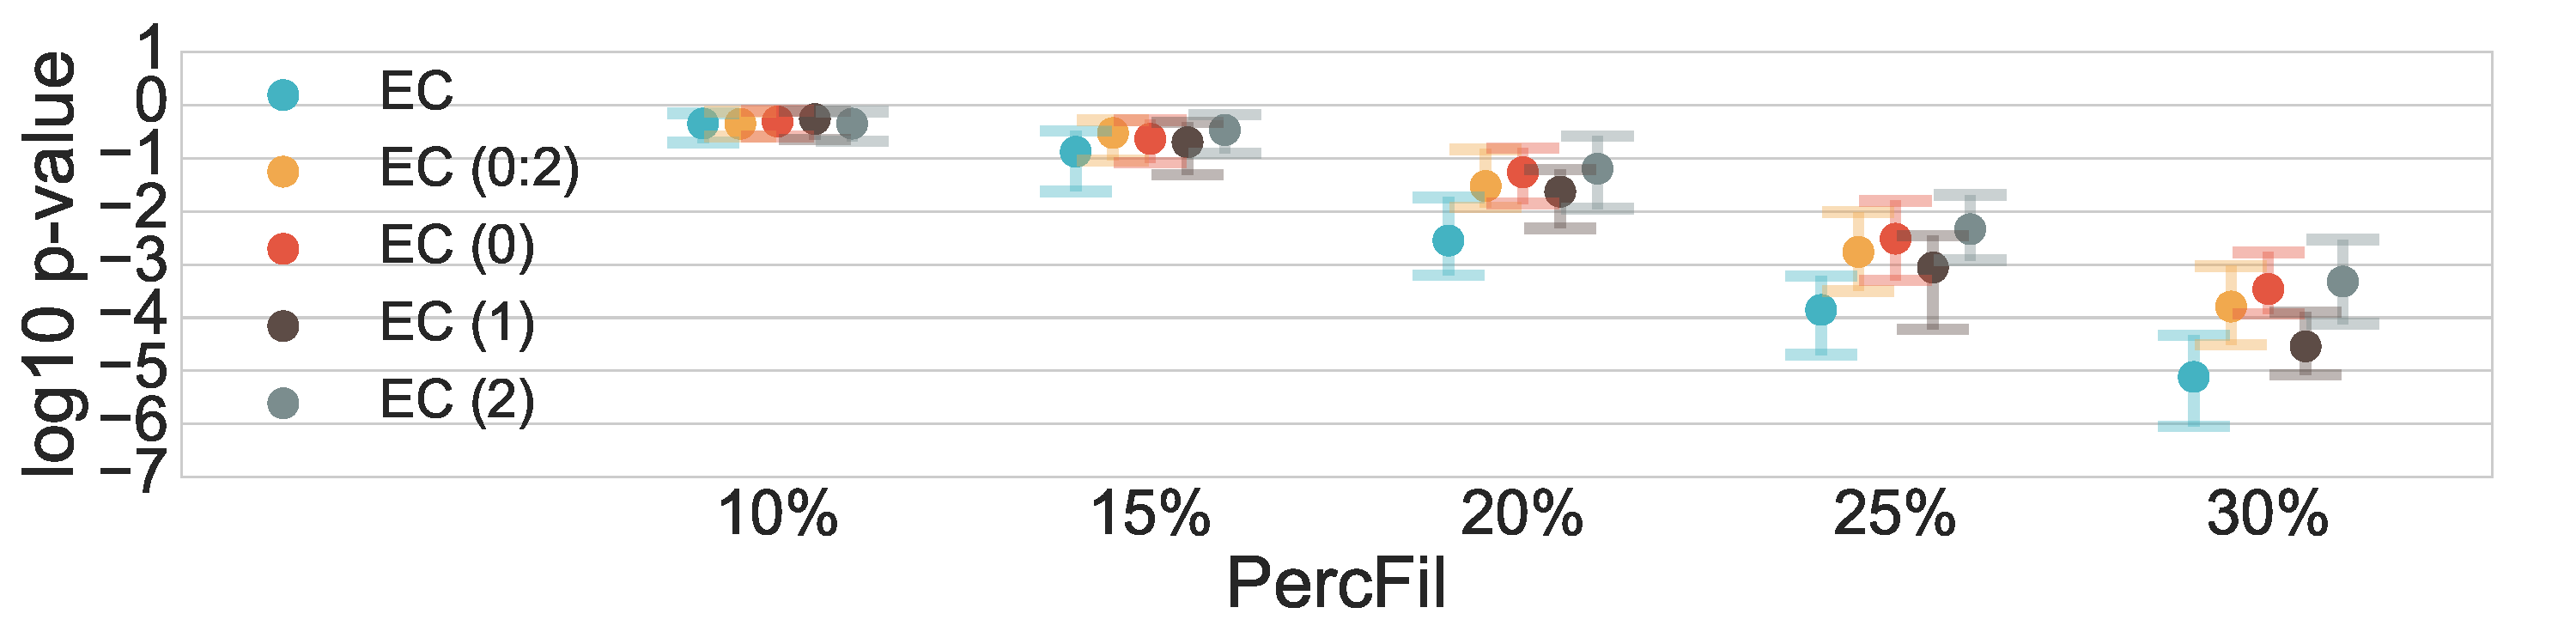
\includegraphics[height = 1.25in]{figure_8_euler_group.pdf}
%     \label{fig:sub_euler}
%   \end{subfigure}
%   \begin{subfigure}{.75\textwidth}
%     \centering
%     \caption{EC Tests (Standardized Ratio)}
%     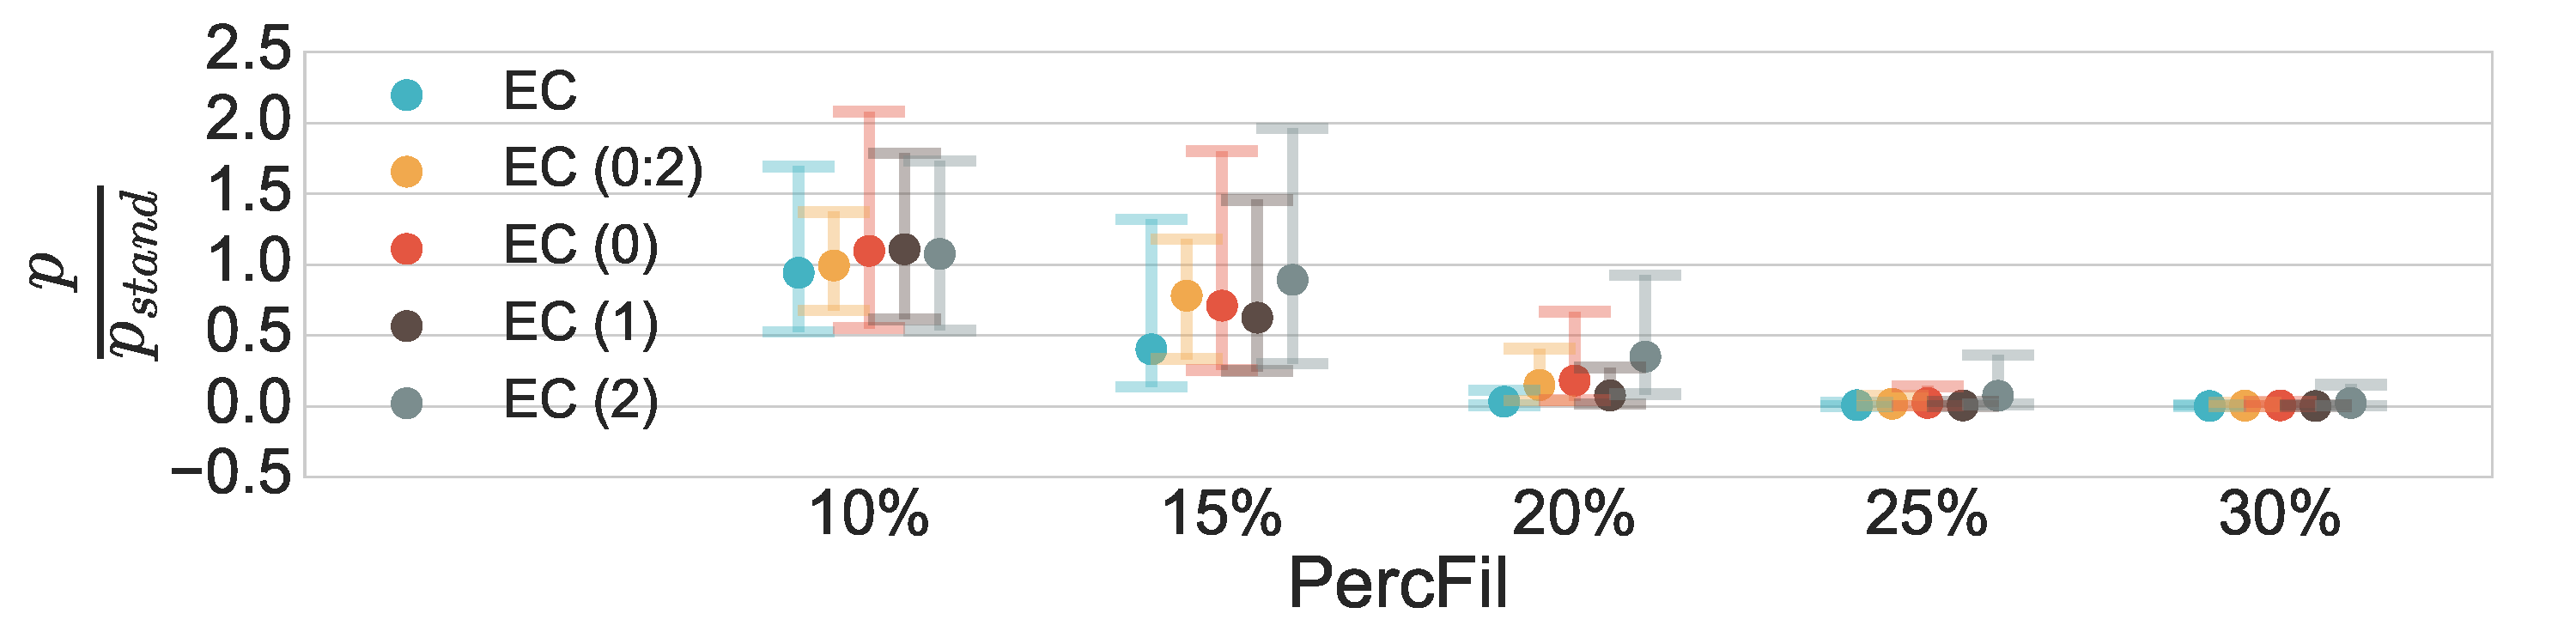
\includegraphics[height = 1.25in]{figure_8_joint_euler_group.pdf}
%     \label{fig:sub_euler_normed}
%   \end{subfigure}
% \caption{(a) Results for the EC tests. X-axis represents the true PercFil (10\%, 15\%, 20\%, 25\%, 30\%) of the second population, compared to the null PercFil of 10\%. The vertical axis shows the $\log_{10}$(p-values). The lines plots the median $\log_{10}$ p-value and error bars show the 25th and 75th percentiles of the 1,000 iterations. (b) plots the ratio of the unstandardized p-value divided by the standardized p-value for each PercFil. }
% \label{fig:sub_euler_results}
% \end{figure}

% \begin{figure}[htp!]
%   \centering
%   \begin{subfigure}{.75\textwidth}
%     \centering
%     \caption{SIL Tests}
%     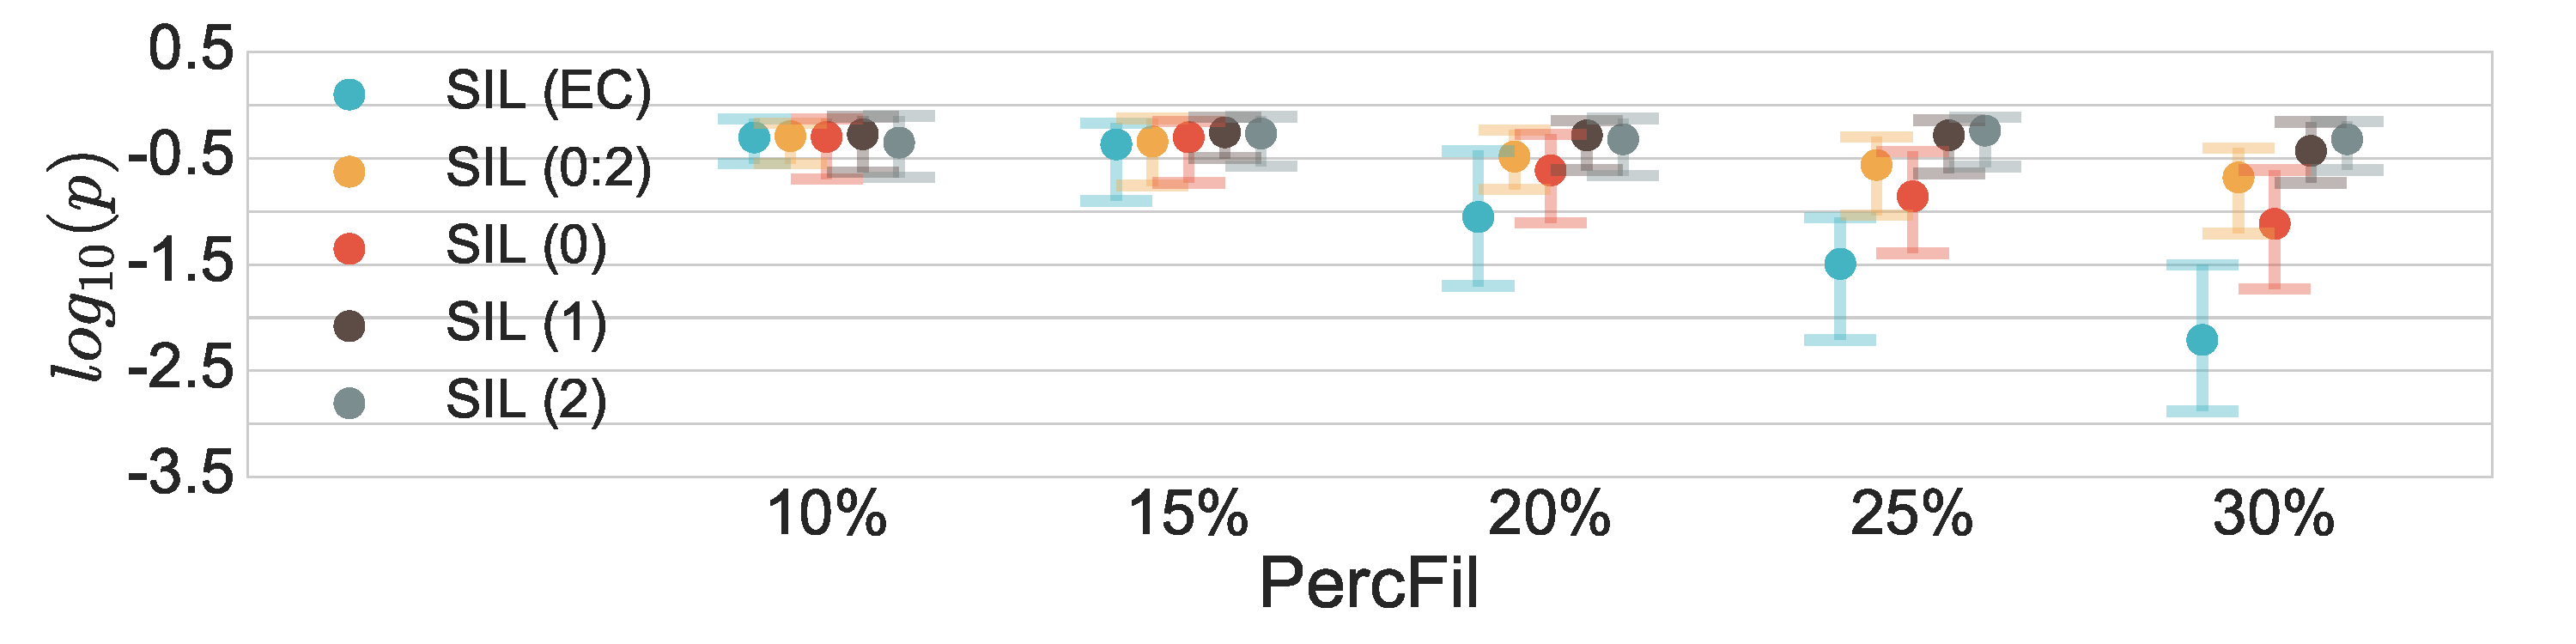
\includegraphics[height = 1.25in]{figure_8_silhouette_group.pdf}
%     \label{fig:sub_silh}
%   \end{subfigure}
%   \begin{subfigure}{.75\textwidth}
%     \centering
%     \caption{SIL Tests (Standardized Ratio)}
%     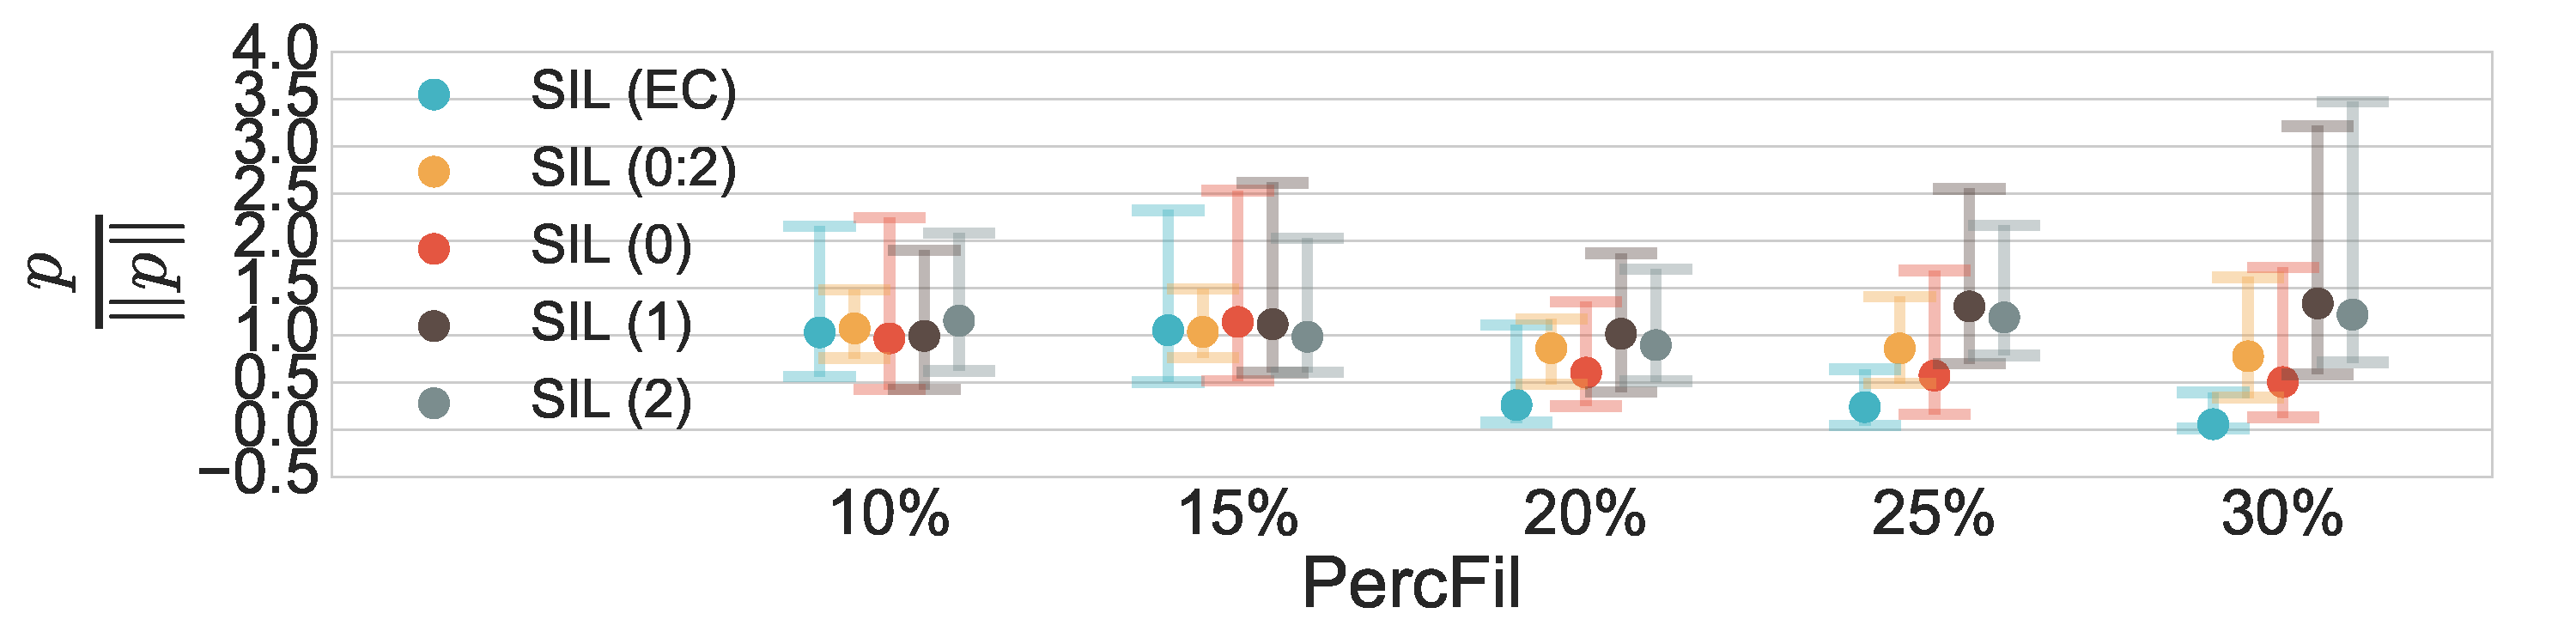
\includegraphics[height = 1.25in]{figure_8_joint_silhouette_group.pdf}
%     \label{fig:sub_silh_normed}
%   \end{subfigure}
% \label{fig:sub_silh_results}
% \caption{(a) Results for the SIL tests. X-axis represents the true PercFil (10\%, 15\%, 20\%, 25\%, 30\%) of the second population, compared to the null PercFil of 10\%. The vertical axis shows the $\log_{10}$(p-values). The lines plots the median $\log_{10}$ p-value and error bars show the 25th and 75th percentiles of the 1,000 iterations. (b) plots the ratio of the unstandardized p-value divided by the standardized p-value for each PercFil. }

% \end{figure}

% \begin{figure}[htp!]
%   \centering
%   \begin{subfigure}{.75\textwidth}
%     \centering
%     \caption{IK Tests}
%     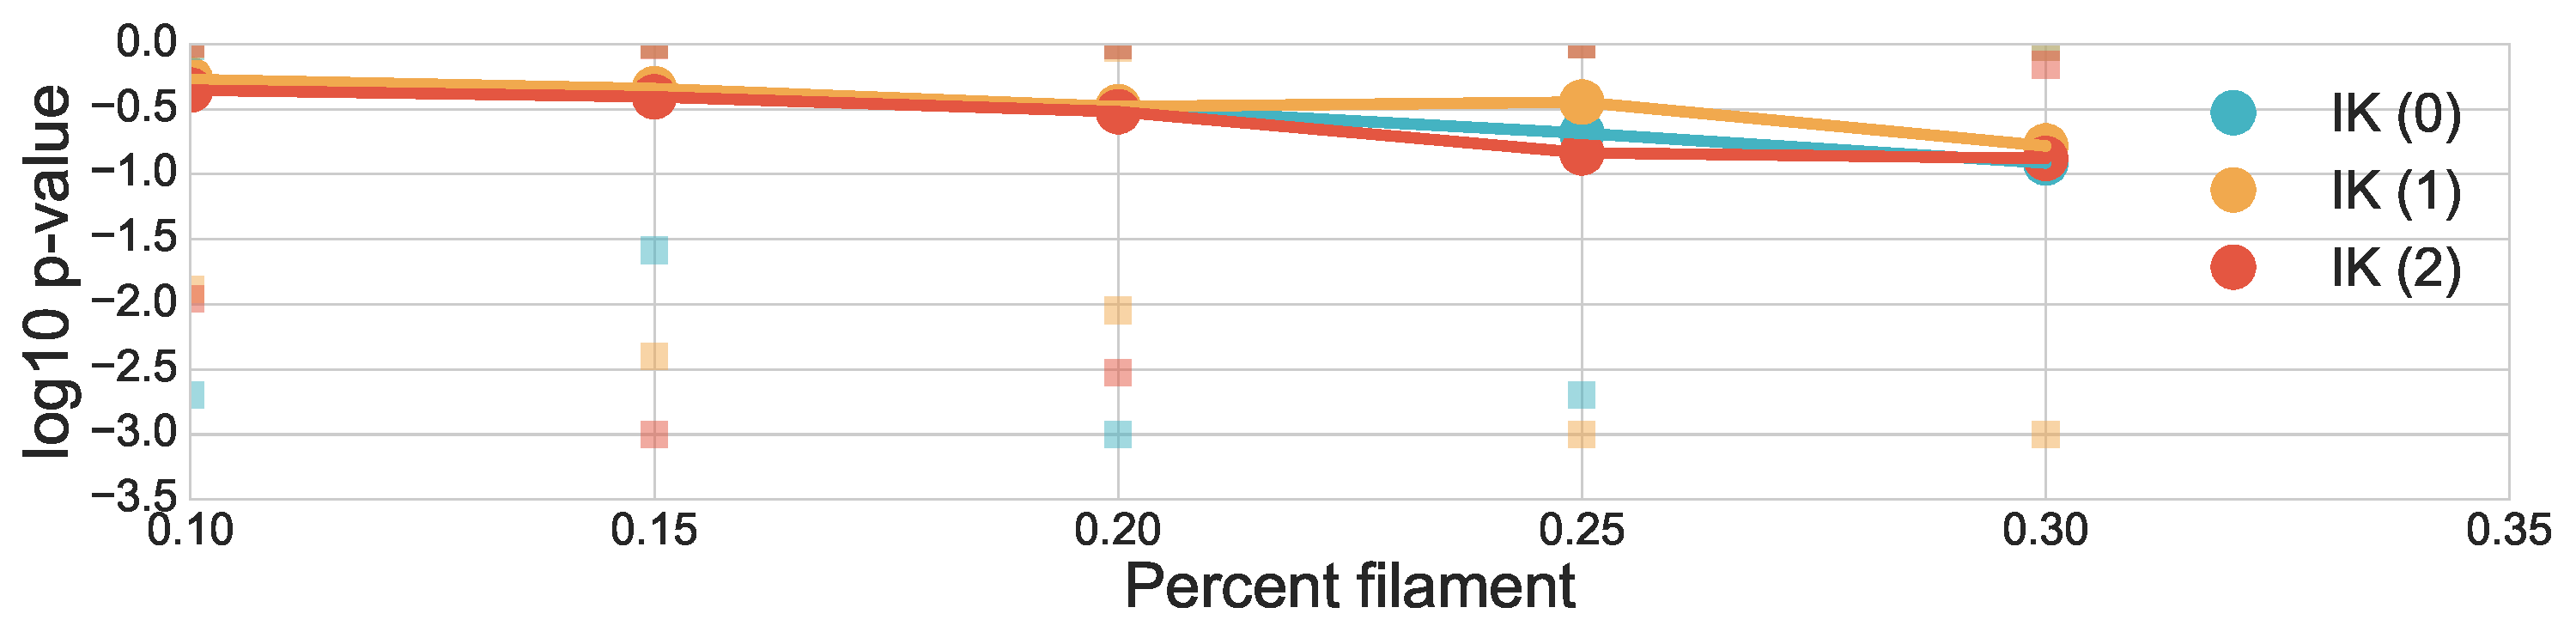
\includegraphics[height = 1.25in]{figure_8_contour_group.pdf}
%     \label{fig:sub_contour}
%   \end{subfigure}
%   \begin{subfigure}{.75\textwidth}
%     \centering
%     \caption{IK Tests (Standardized Ratio)}
%     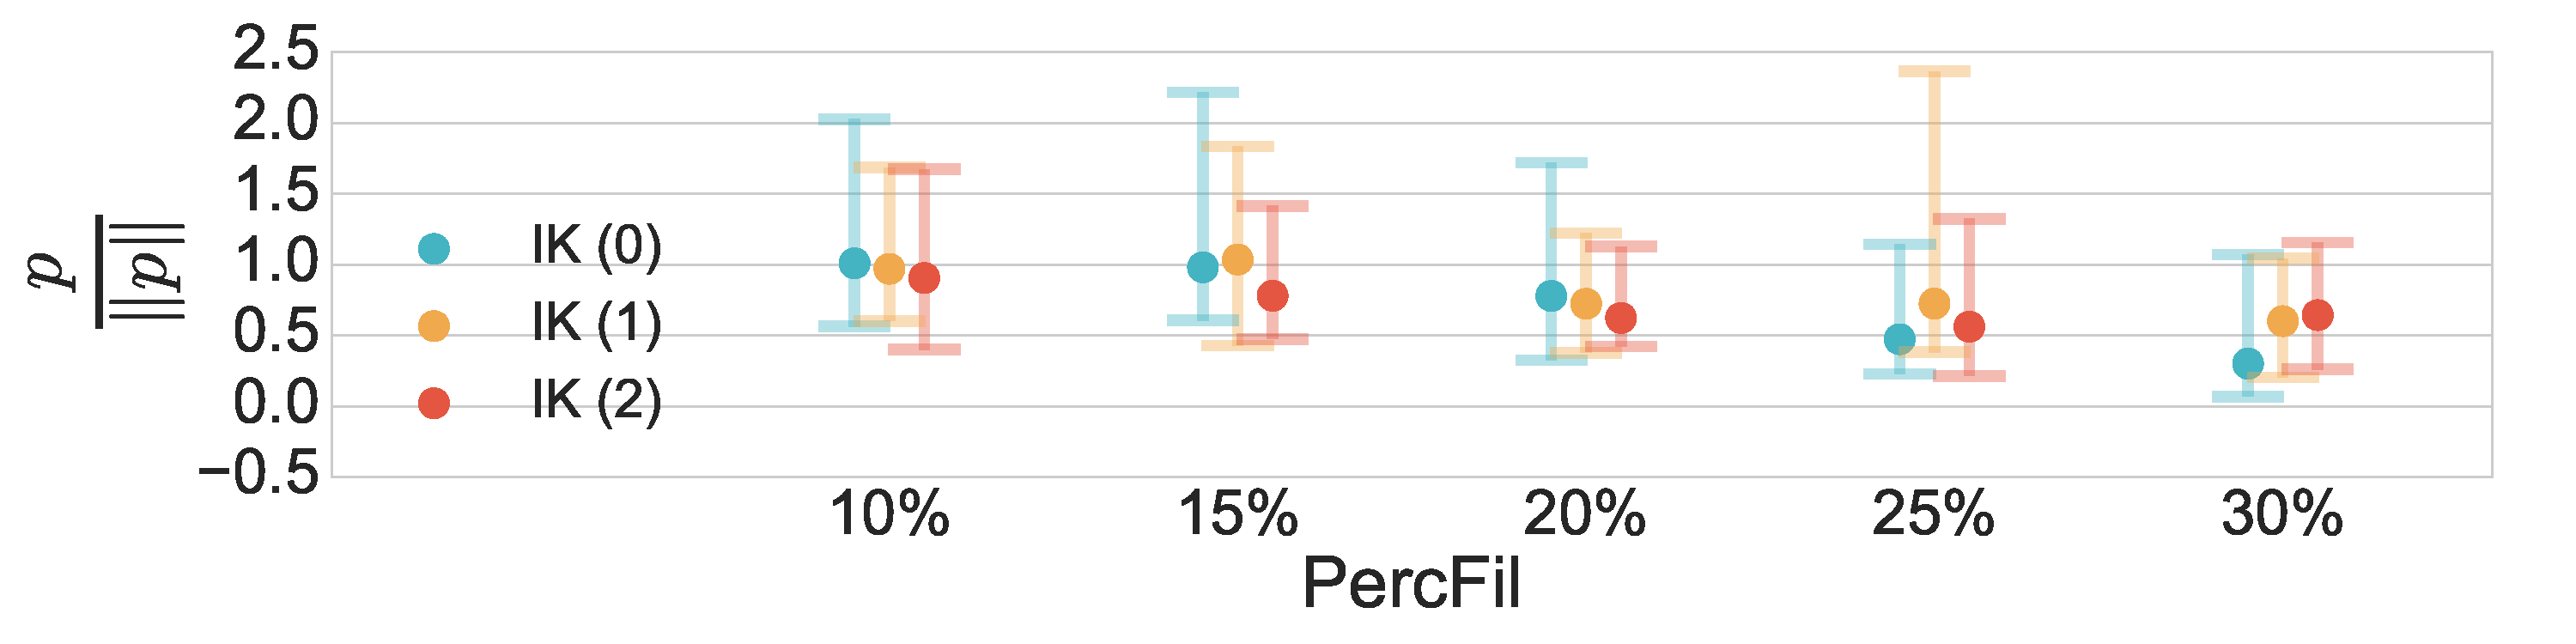
\includegraphics[height = 1.25in]{figure_8_joint_contour_group.pdf}
%     \label{fig:sub_contour_normed}
%   \end{subfigure}
% \label{fig:sub_contour_results}
% \caption{(a) Results for the IK tests. X-axis represents the true PercFil (10\%, 15\%, 20\%, 25\%, 30\%) of the second population, compared to the null PercFil of 10\%. The vertical axis shows the $\log_{10}$(p-values). The lines plots the median $\log_{10}$ p-value and error bars show the 25th and 75th percentiles of the 1,000 iterations. (b) plots the ratio of the unstandardized p-value divided by the standardized p-value for each PercFil. }
% \end{figure}

% \begin{figure}[htp!]
%   \centering
%   \begin{subfigure}{.75\textwidth}
%     \centering
%     \caption{WIK/PI Tests}
%     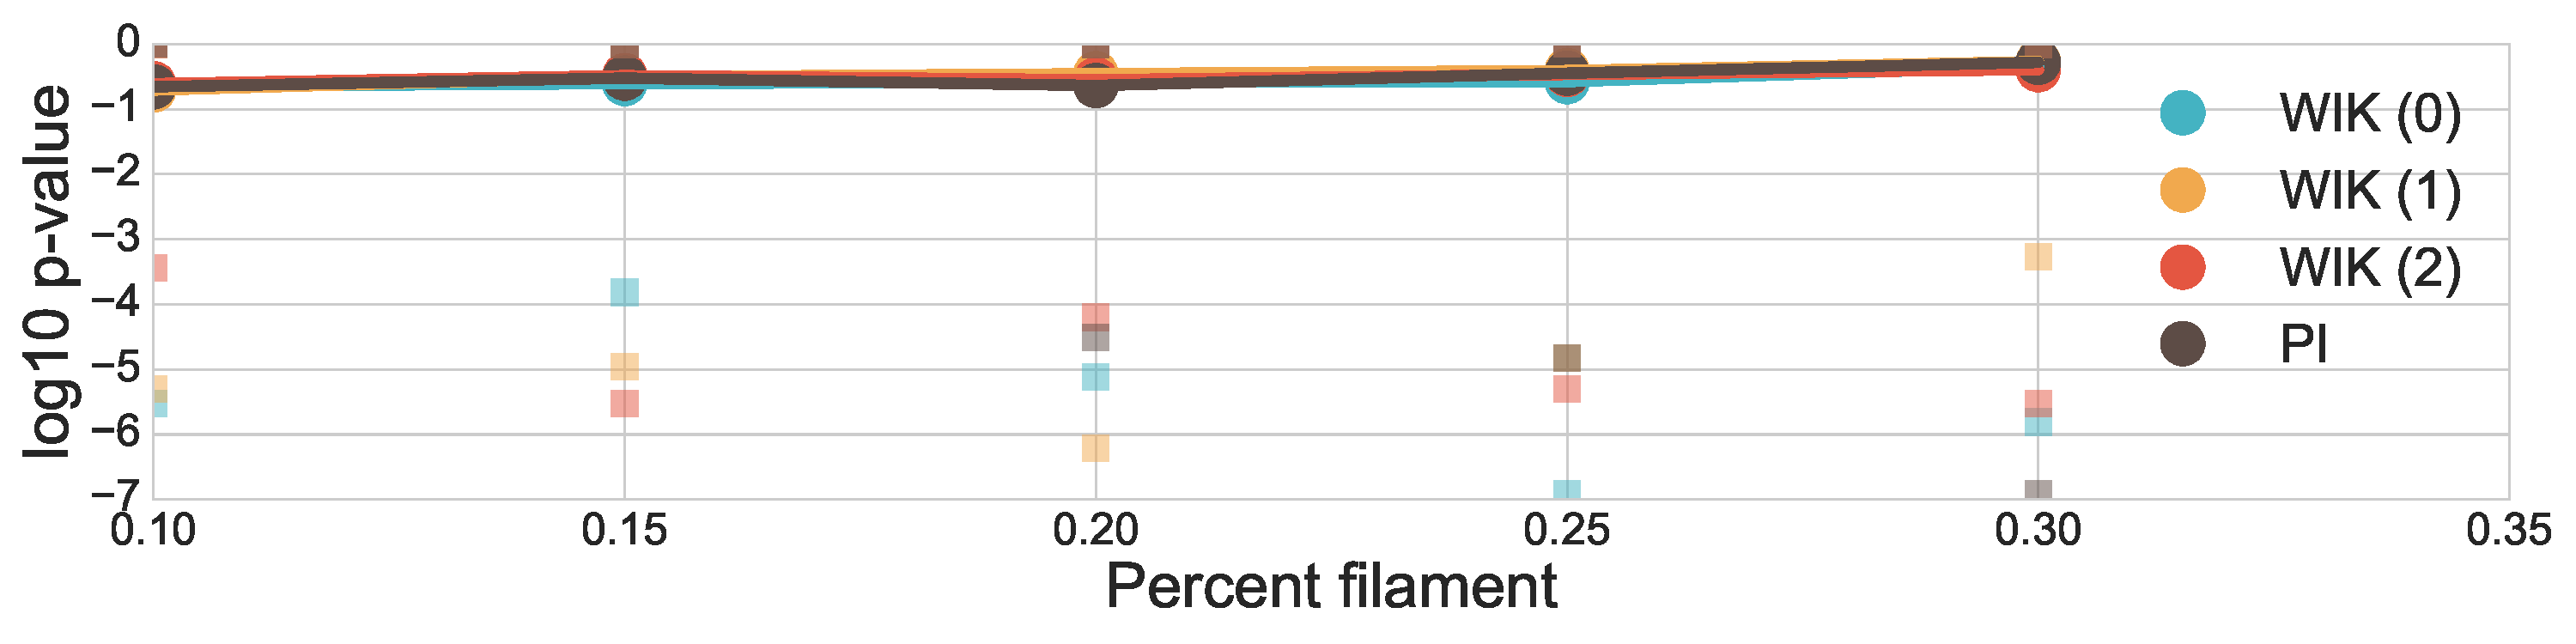
\includegraphics[height = 1.25in]{figure_8_weighted_contour_group.pdf}
%     \label{fig:sub_weight}
%   \end{subfigure}
%   \begin{subfigure}{.75\textwidth}
%     \centering
%     \caption{WIK/PI Tests (Standardized Ratio)}
%     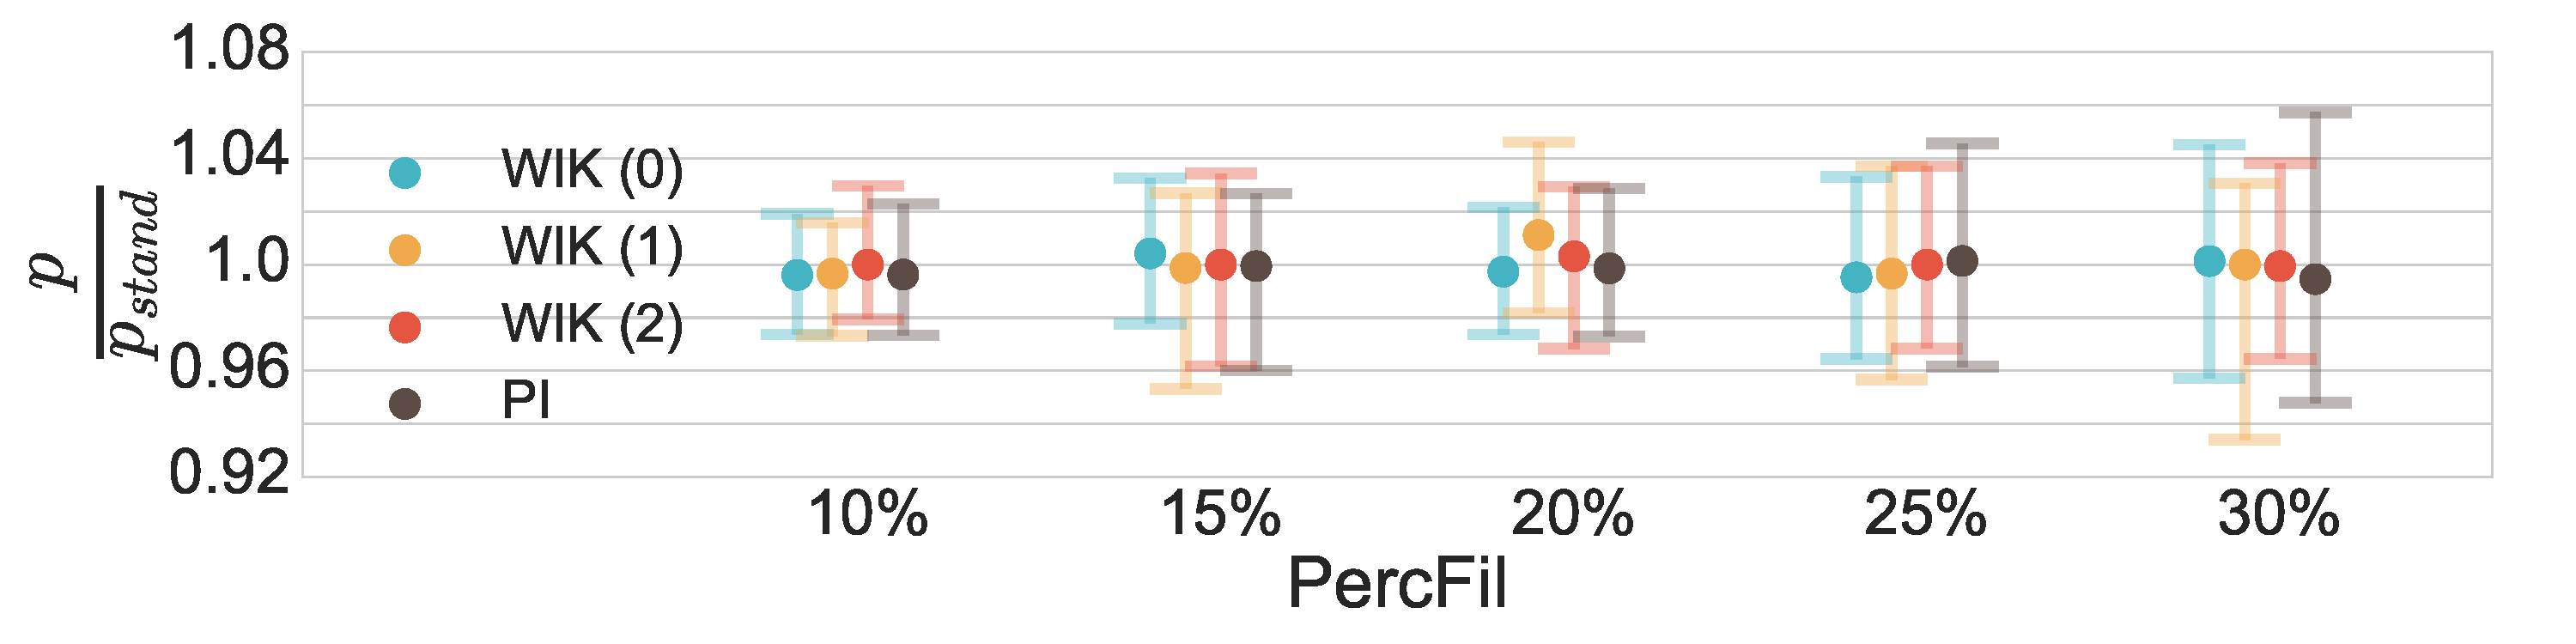
\includegraphics[height = 1.25in]{figure_8_joint_weighted_contour_group.pdf}
%     \label{fig:sub_weight_normed}
%   \end{subfigure}
% \label{fig:sub_weight_results}
% \caption{(a) Results for the WIK/PI tests. X-axis represents the true PercFil (10\%, 15\%, 20\%, 25\%, 30\%) of the second population, compared to the null PercFil of 10\%. The vertical axis shows the $\log_{10}$(p-values). The lines plots the median $\log_{10}$ p-value and error bars show the 25th and 75th percentiles of the 1,000 iterations. (b) plots the ratio of the unstandardized p-value divided by the standardized p-value for each PercFil. }

% \end{figure}

% \begin{figure}[htp!]
%   \centering
%   \begin{subfigure}{.75\textwidth}
%     \caption{CORR Tests}
%     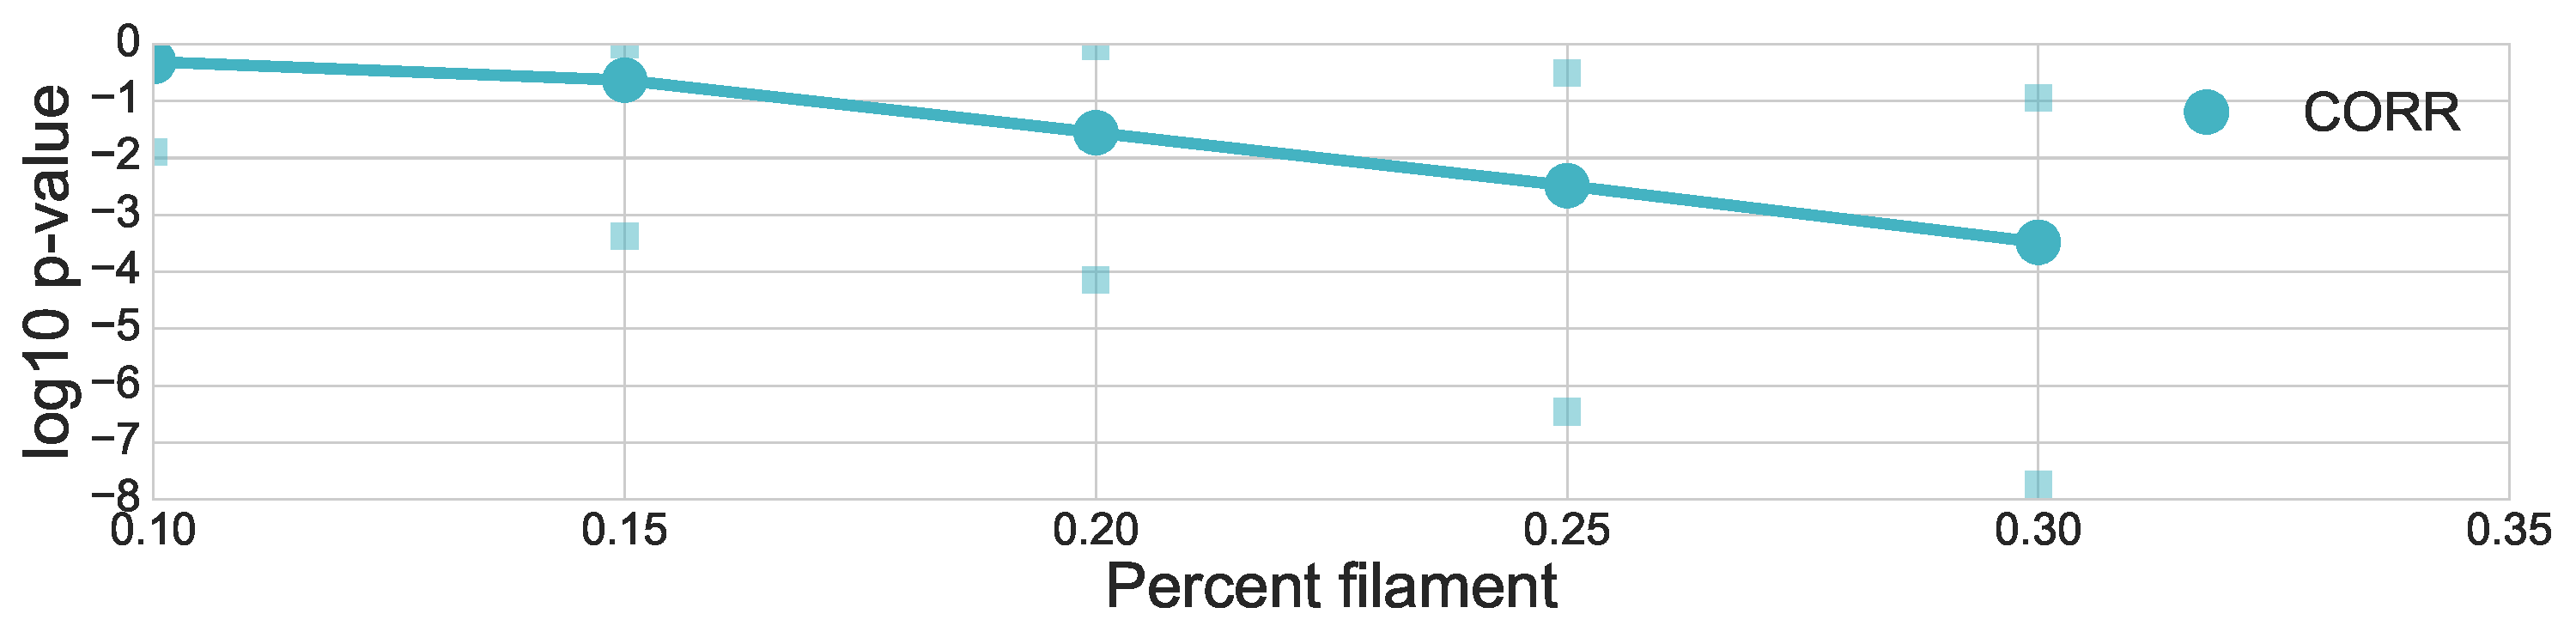
\includegraphics[height = 1.25in]{figure_8_correlation_group.pdf}
%     \label{fig:sub_corr}
%   \end{subfigure}
%   \begin{subfigure}{.75\textwidth}
%     \caption{CORR Tests (Standardized Ratio)}
%     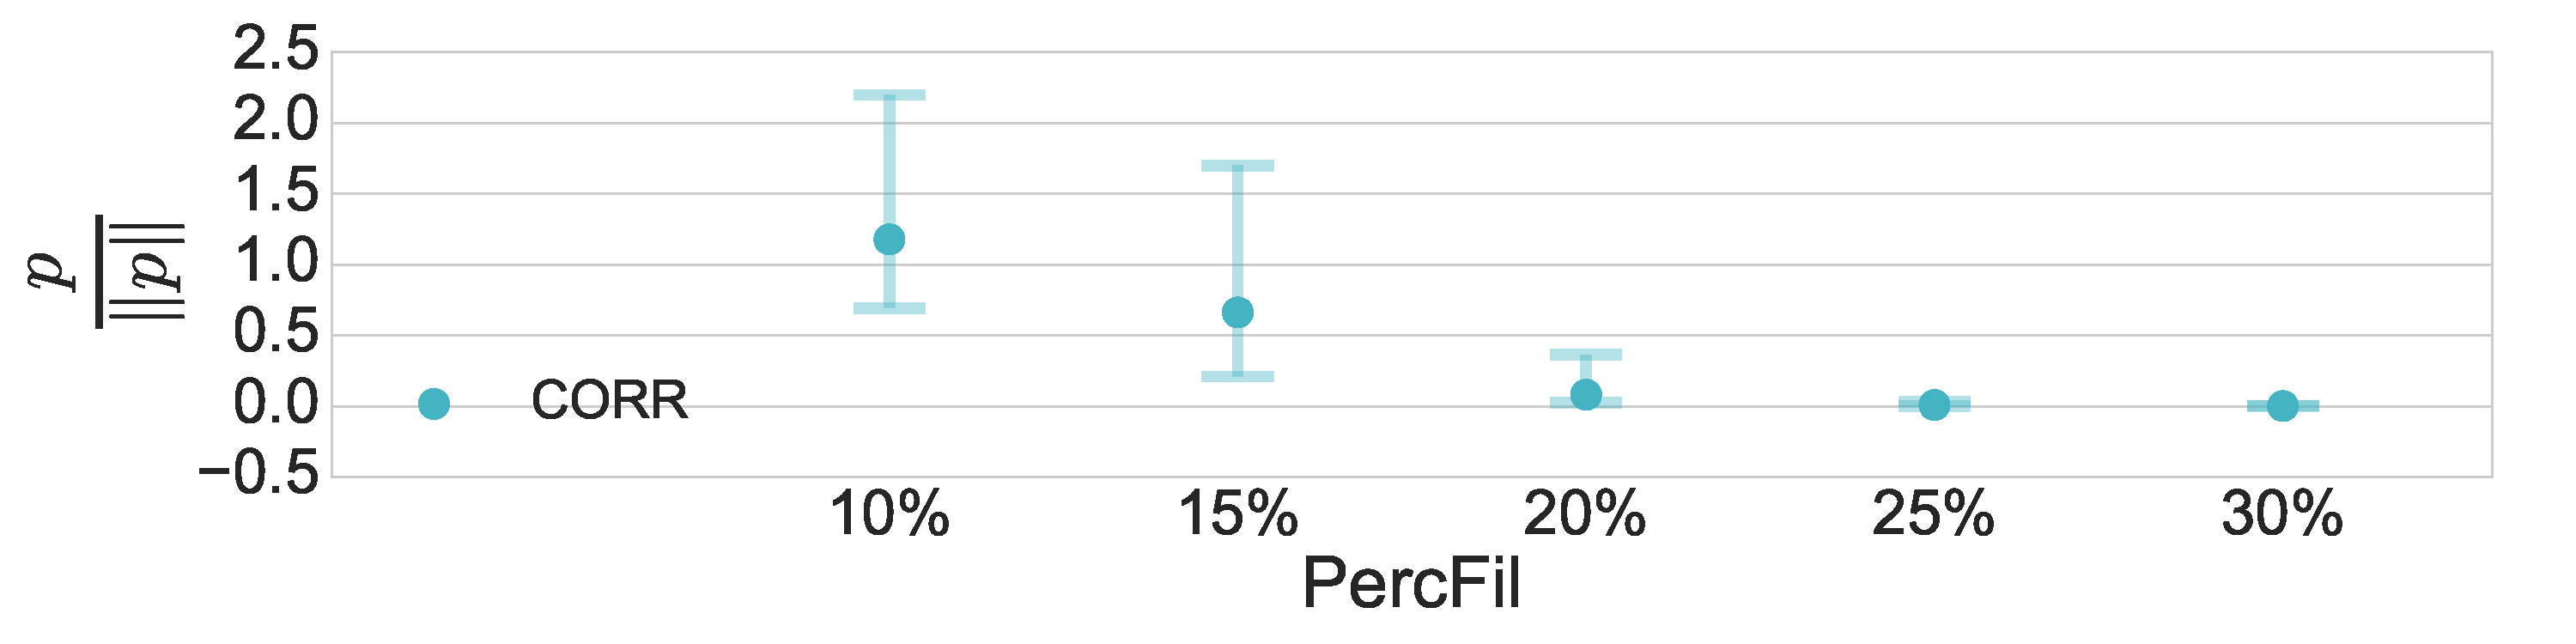
\includegraphics[height = 1.25in]{figure_8_joint_correlation_group.pdf}
%     \label{fig:sub_corr_normed}
%   \end{subfigure}
% \caption{(a) Results for the CORR tests. X-axis represents the true PercFil (10\%, 15\%, 20\%, 25\%, 30\%) of the second population, compared to the null PercFil of 10\%. The vertical axis shows the $\log_{10}$(p-values). The lines plots the median $\log_{10}$ p-value and error bars show the 25th and 75th percentiles of the 1,000 iterations. (b) plots the ratio of the unstandardized p-value divided by the standardized p-value for each PercFil. }
% \label{fig:sub_corr_results_2}
% \end{figure}

% --------------- END FIGURES -----------------



\subsubsection{Standardization of persistence diagrams} \label{sec:standardize}
In the methods proposed above, difference in scale can also result in rejection when, in fact there are not statistically significant topological differences. For example, suppose we are considering two datasets - each has points randomly sampled from the perimeter of a circle with a radius of 1 and 10 respectively. It may or may not be desirable to conclude that the two datasets come from different persistence diagram generators (i.e. conclude $\mathcal P^{(1)} \neq \mathcal P^{(2)}$) since inference would be based on geometrical (scaling) differences rather than topological differences. If we wish to focus only on topological differences, we propose a possible preprocessing step to normalize scaling. Specifically, we standardize the persistence diagrams so that all the homological features are re-scaled to $[0, 1]\times[0,1]$. This simple standardization takes the persistence diagram window and shrinks it or expands it to fill the $[0, 1]\times[0,1]$ window, maintaining the same relationship among all the homological features. If there is concern about outliers, then other quantiles could be used for the standardization. The exception is with the CORR, in which the point cloud itself is standardized to $[0, 1]\times[0, 1]\times[0, 1]$.

We repeated the simulation study from \S \ref{sec:results1} except including our standardization; the results are displayed in \figref{fig:subLinesNormApp}. Standardization had an appreciable impact on hypothesis test results, decreasing the effectiveness and sensitivity of all test statistics. Notice, however, that the best-performing test statistics remain the same: EC, CORR, SILEC tests, confirming that the properties underlying those three tests are better able to capture purely topological differences than any other test presented in this paper. Notably after standardization, the KC, WIK, and other SIL tests have essentially constant p-values across the percFil variation, losing effectiveness in distinguishing differences. One interpretation may be that these tests captured only geometric dissimilarities in the unstandardized setting.



% --------------- BEGIN FIGURES -----------------

\begin{center}
  \begin{figure}[htp!]
    \centering
%    \begin{subfigure}{.48\textwidth}
%      \centering
%      \caption{EC Tests}
%      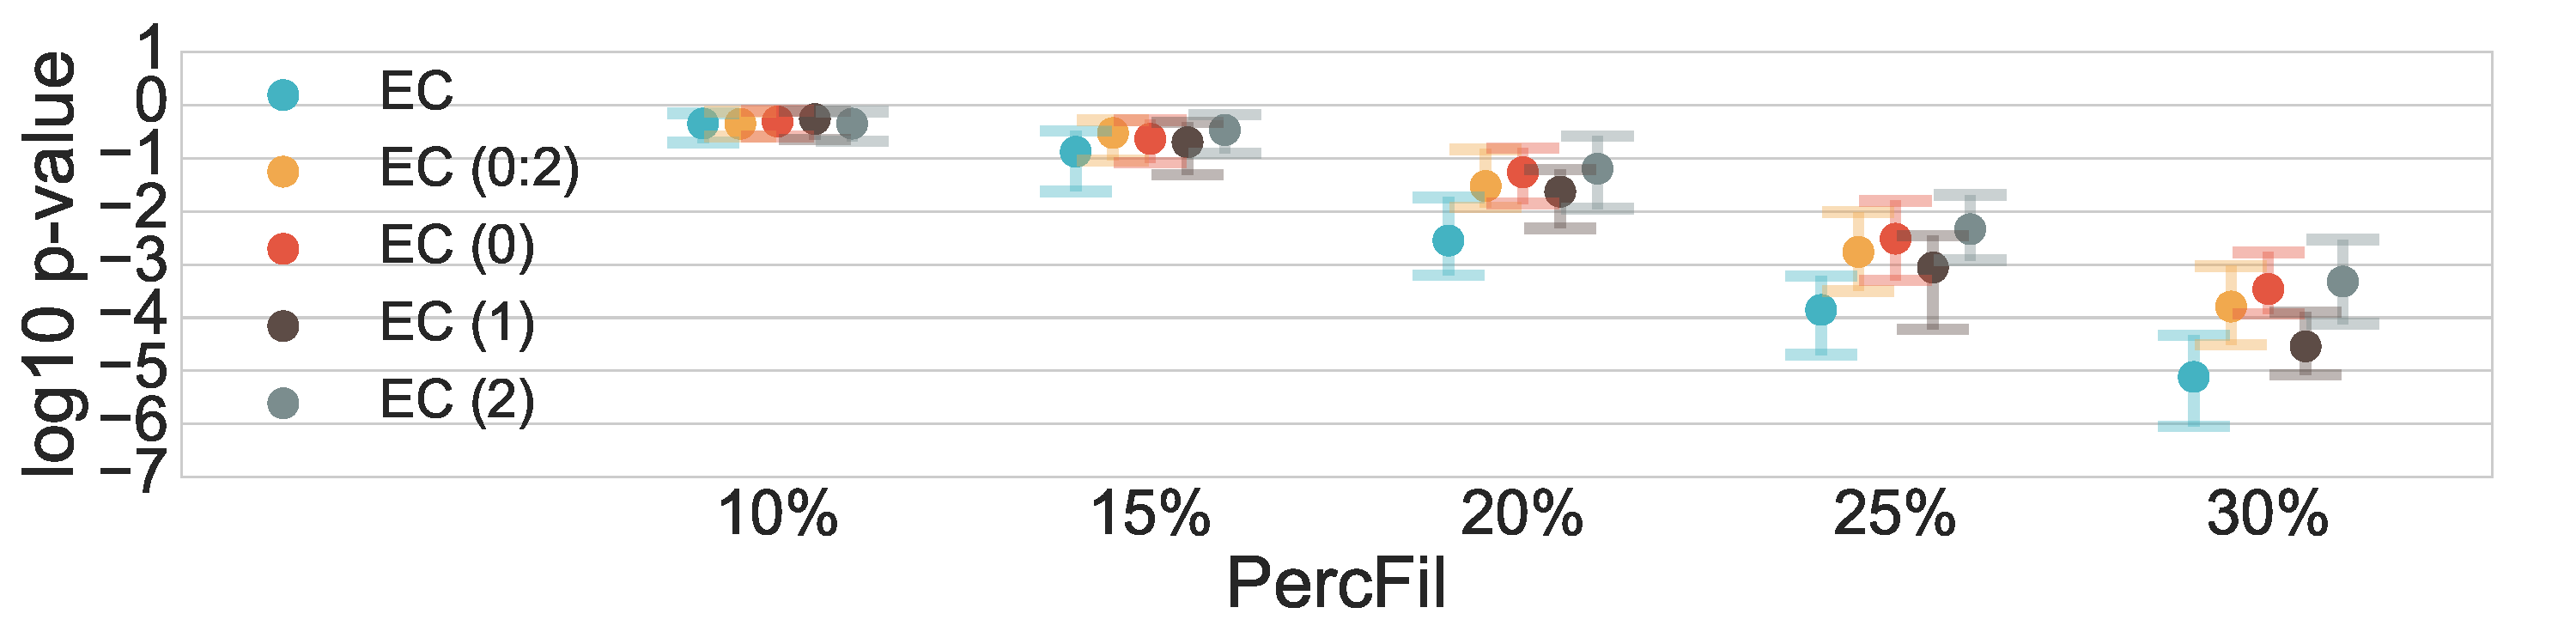
\includegraphics[width=\linewidth, height = .75in]{figure_8_euler_group.pdf}
%      \label{fig:sub_euler}
%    \end{subfigure}
    \begin{subfigure}{.47\textwidth}
      \centering
      \caption{EC Tests (Standardized Ratio)}
      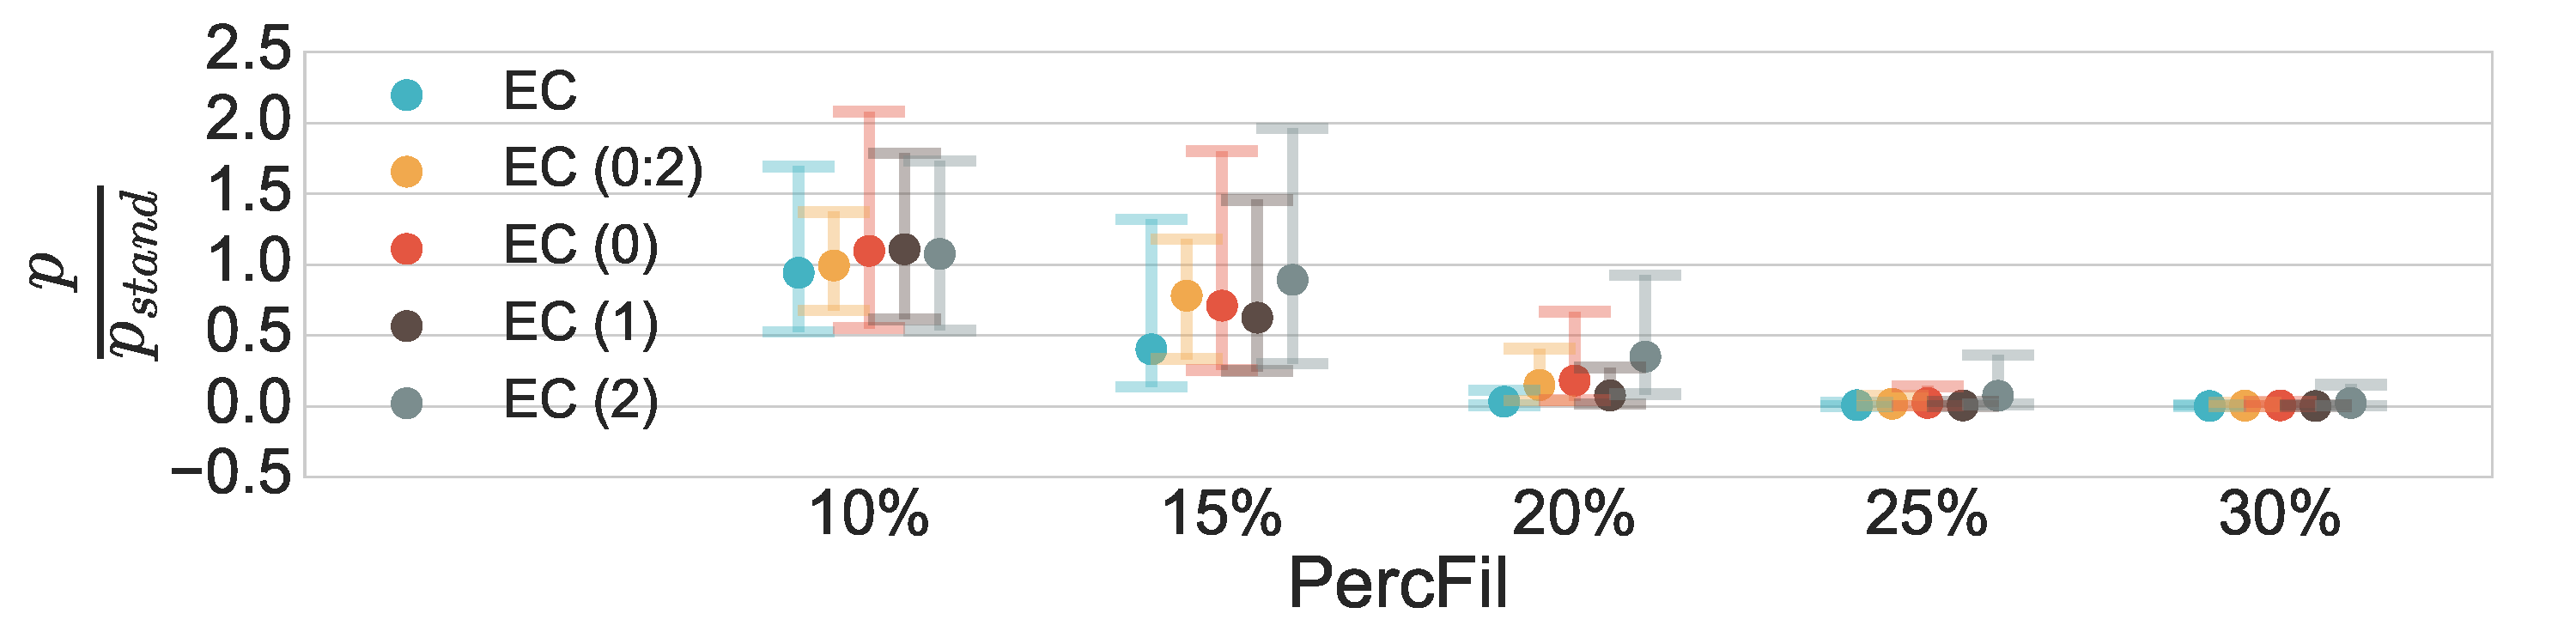
\includegraphics[height = .78in]{figure_8_joint_euler_group.pdf}
      \label{fig:sub_euler_normed}
    \end{subfigure}
%    \begin{subfigure}{.48\textwidth}
%      \centering
%      \caption{SIL Tests}
%      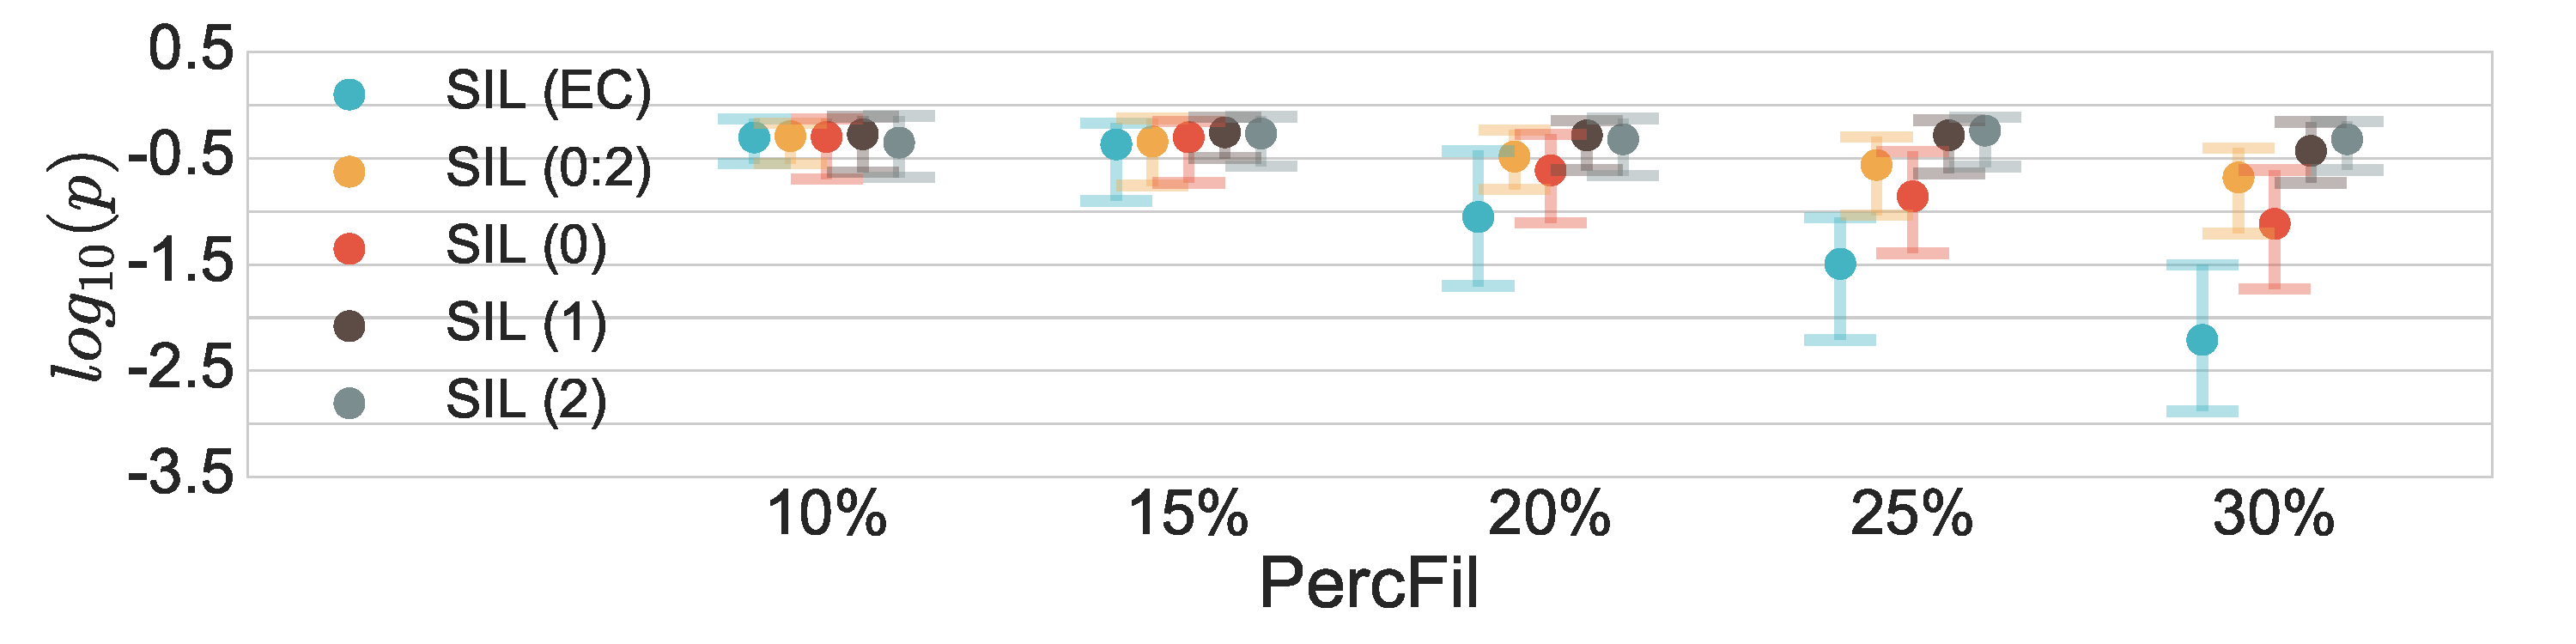
\includegraphics[width=\linewidth, height = .75in]{figure_8_silhouette_group.pdf}
%      \label{fig:sub_silh}
%    \end{subfigure}
    \begin{subfigure}{.47\textwidth}
      \centering
      \caption{SIL Tests (Standardized Ratio)}
      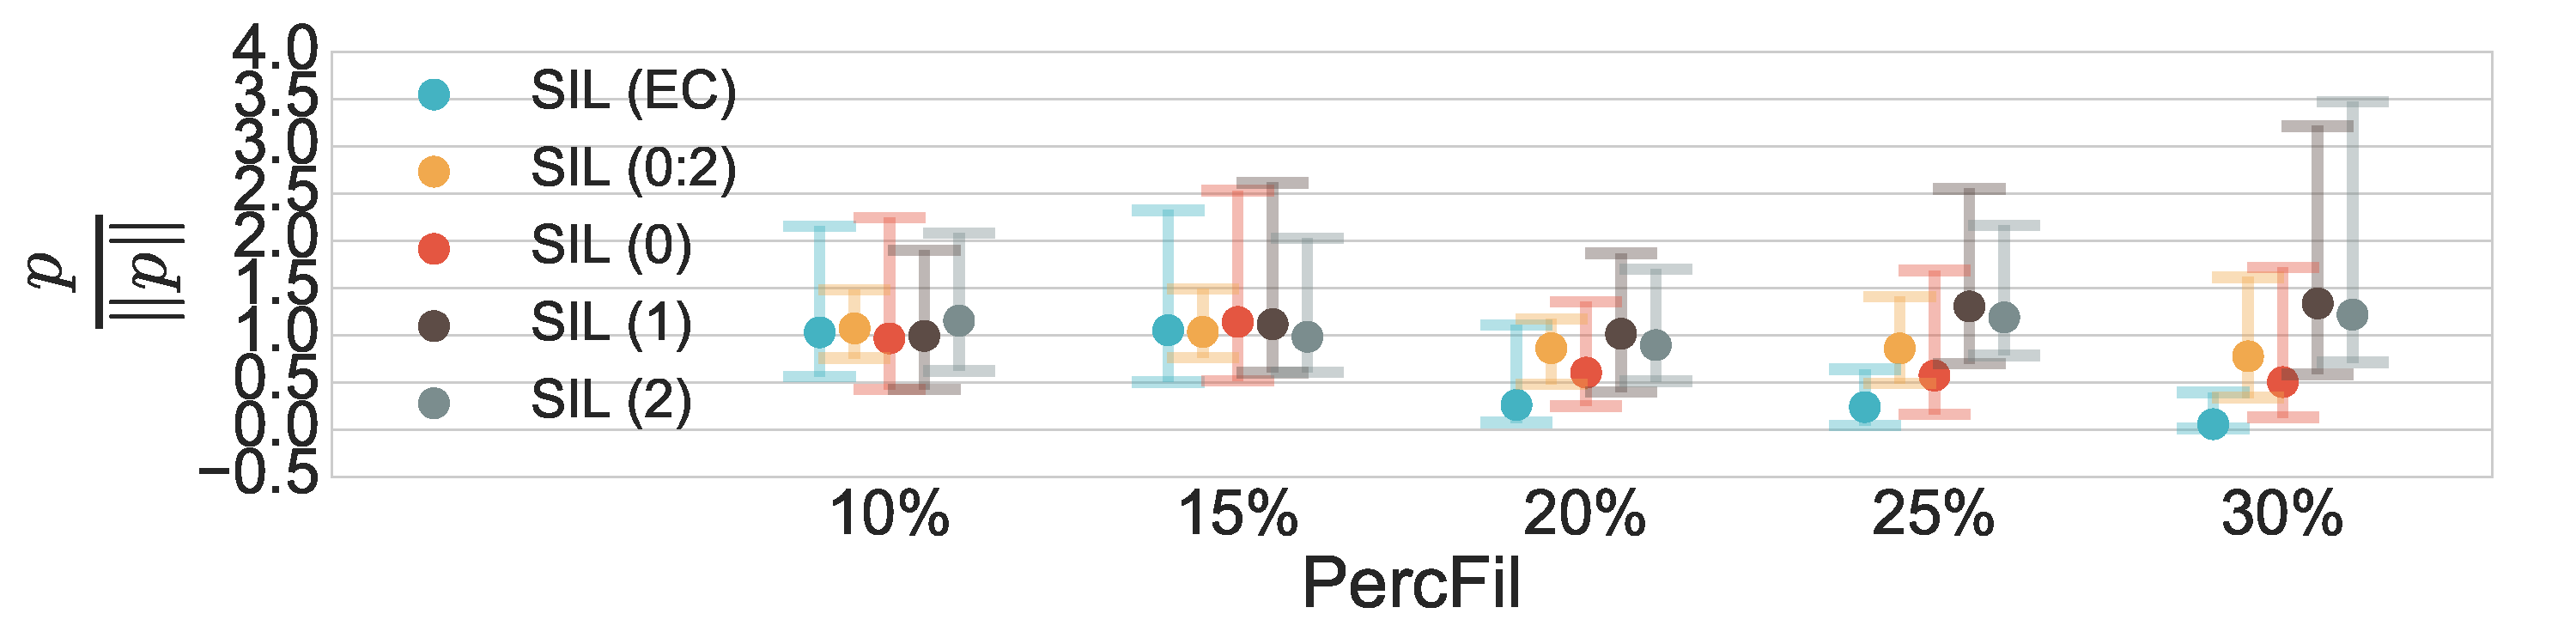
\includegraphics[height = .78in]{figure_8_joint_silhouette_group.pdf}
      \label{fig:sub_silh_normed_normed}
    \end{subfigure}
%    \begin{subfigure}{.48\textwidth}
%      \centering
%      \caption{IK Tests}
%      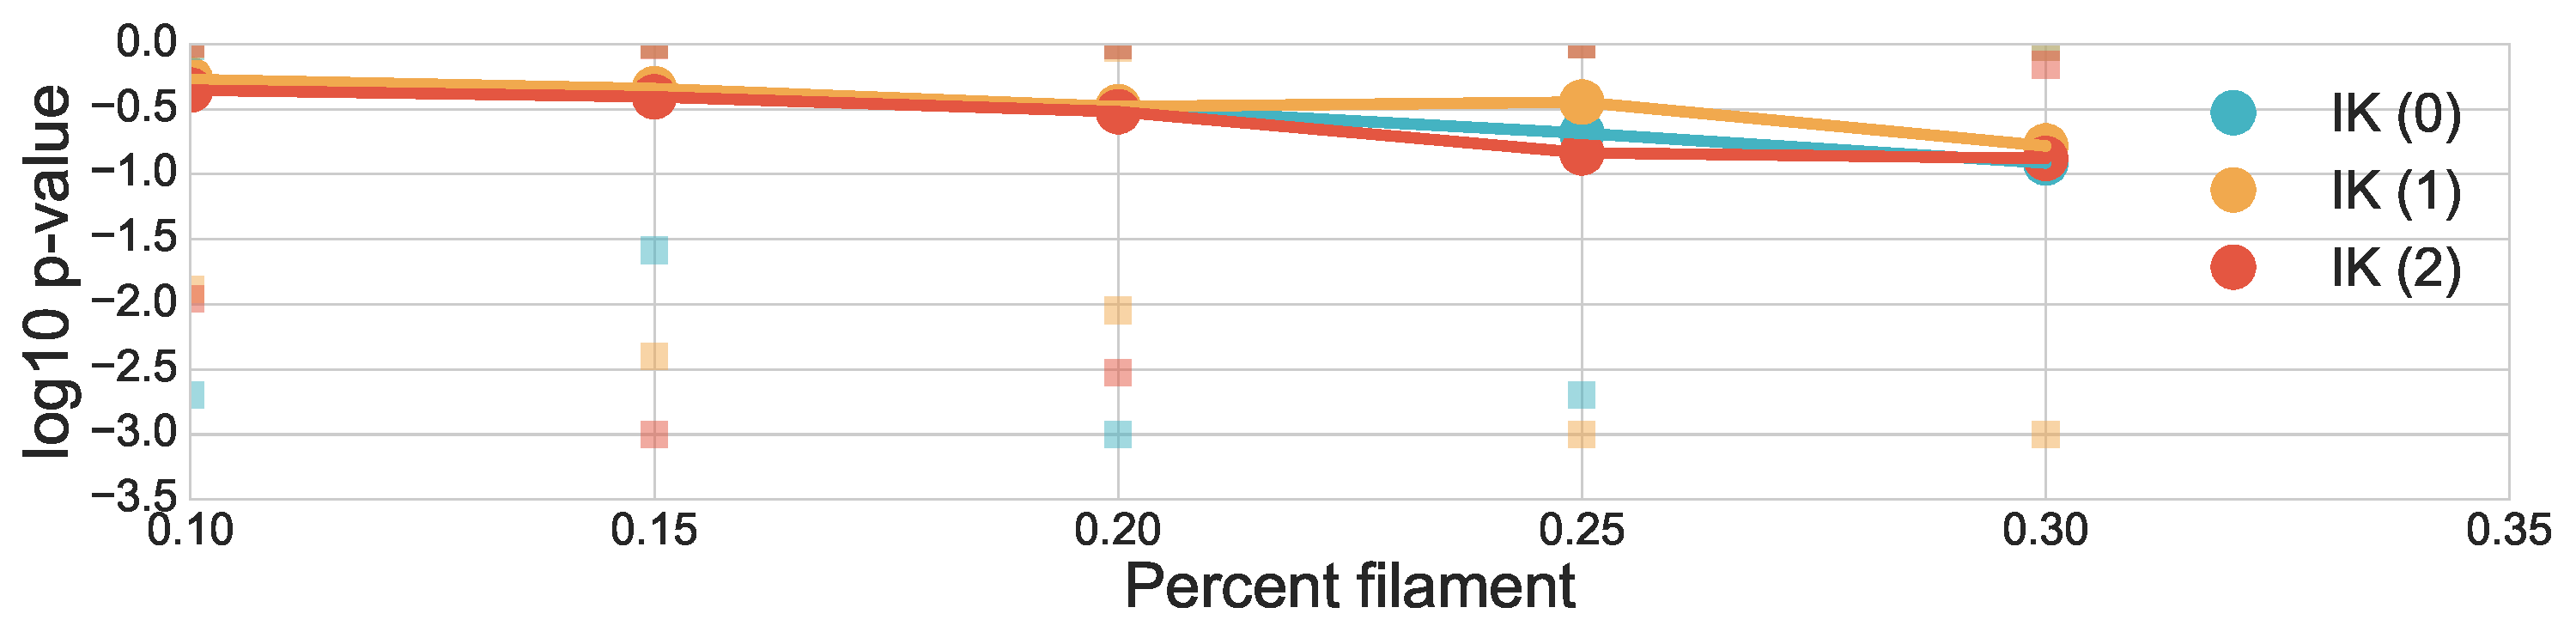
\includegraphics[width=\linewidth, height = .75in]{figure_8_contour_group.pdf}
%      \label{fig:sub_contour}
%    \end{subfigure}
    \begin{subfigure}{.47\textwidth}
      \centering
      \caption{IK Tests (Standardized Ratio)}
      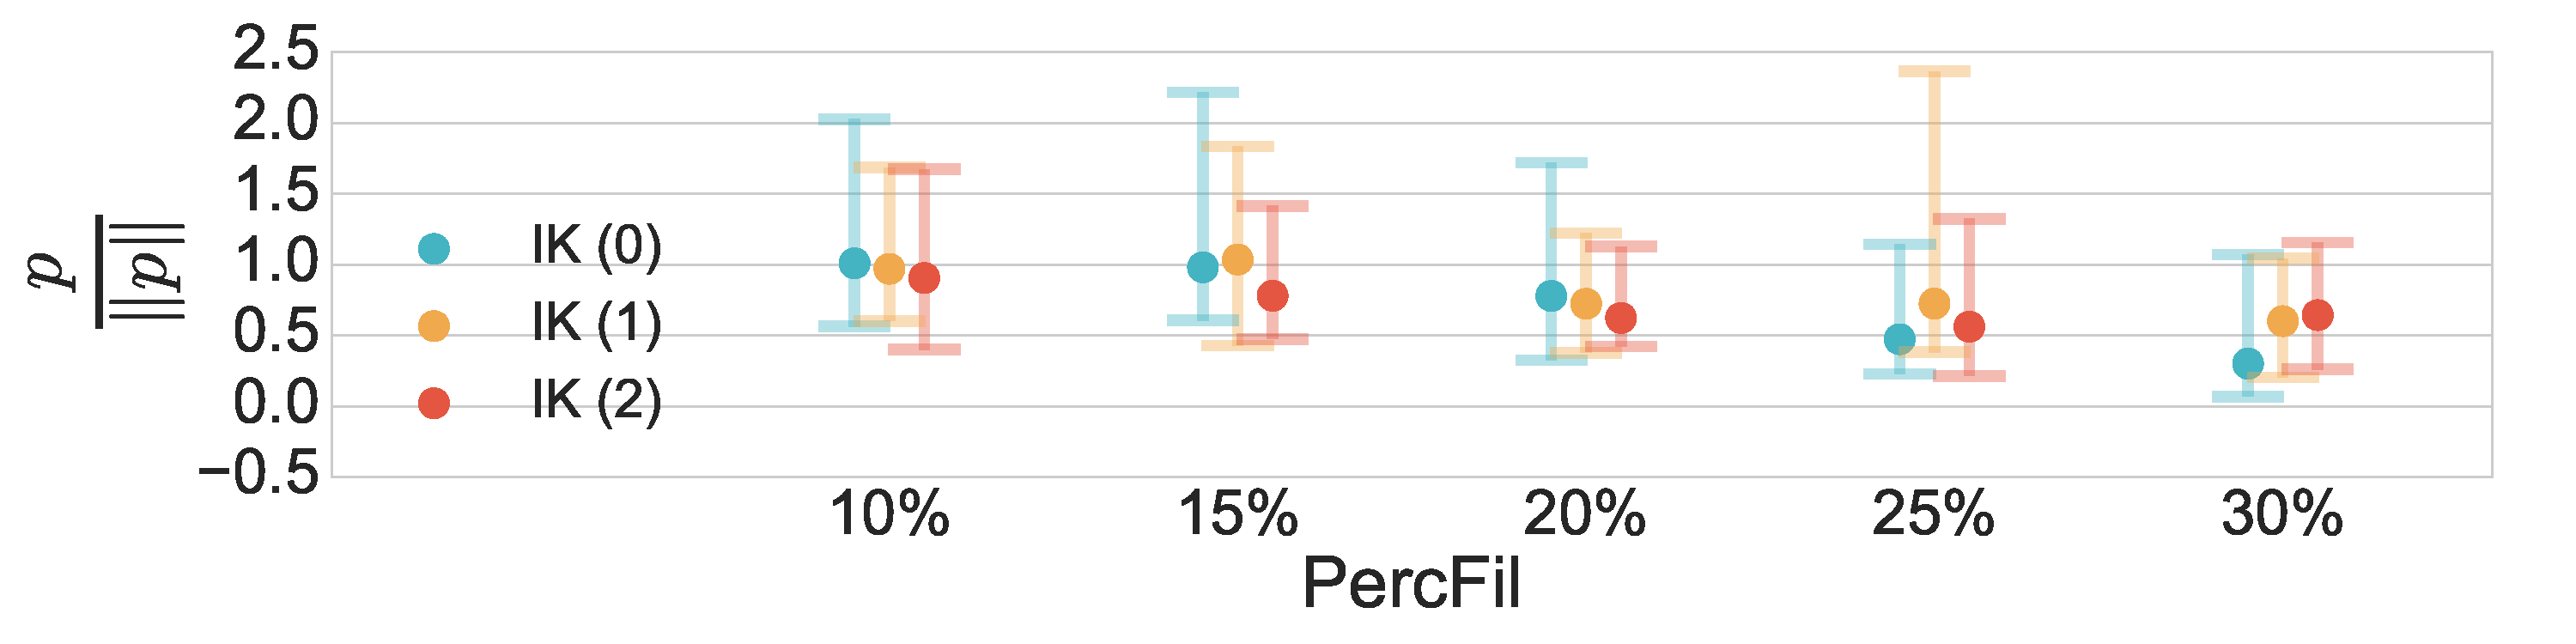
\includegraphics[height = .78in]{figure_8_joint_contour_group.pdf}
      \label{fig:sub_contour_normed}
    \end{subfigure}
%    \begin{subfigure}{.48\textwidth}
%      \centering
%      \caption{WIK/PI Tests}
%      \includegraphics[width=\linewidth, height = .75in]{figure_8_weighted_contour_group.pdf}
%      \label{fig:sub_weight}
%    \end{subfigure}
    \begin{subfigure}{.47\textwidth}
      \centering
      \caption{WIK/PI Tests (Standardized Ratio)}
      \includegraphics[height = .78in]{figure_8_joint_weighted_contour_group.pdf}
      \label{fig:sub_weight_normed}
    \end{subfigure}
%    \begin{subfigure}{.48\textwidth}
%      \caption{CORR Tests}
%      \includegraphics[width=\linewidth, height = .75in]{figure_8_correlation_group.pdf}
%      \label{fig:sub_corr}
%    \end{subfigure}
    \begin{subfigure}{.47\textwidth}
      \caption{CORR Tests (Standardized Ratio)}
      \includegraphics[height = .78in]{figure_8_joint_correlation_group.pdf}
      \label{fig:sub_corr_normed}
    \end{subfigure}
    \caption{Results for EC, SIL, IK, WIK, PI, and CORR tests. X-axis represents the true PercFil (10\%, 15\%, 20\%, 25\%, 30\%), compared to the null PercFil of 10\%; The vertical axis shows the ration of the unstandardized p-values (from Figure~\ref{fig:subLinesUnnormApp}) over the standardized p-values. The lines plots the median ratio and the error bars show the 25th and 75th percentiles of the 1000 iterations. 
    }
    \label{fig:subLinesNormApp}
  \end{figure}
\end{center}

%%%%%%%%%%%%%%%%%%%%%%%%%%%%%%%%%%%%%%%%%%%%%%%%%%%%%%%
%% SECTION: APPLICATION
%%%%%%%%%%%%%%%%%%%%%%%%%%%%%%%%%%%%%%%%%%%%%%%%%%%%%%%

\section{Application: Cosmological Simulation Data}
\label{sec:application}

In order to study differences in LSS under varying cosmological models, cosmologists run large-scale, computationally intensive simulations using the varying cosmological model settings as inputs.  In this work, we are interested in how the LSS under the assumption of CDM compares to the LSS under the assumption of WDM.
We analyze the N-body simulations of structure formation displayed in Figure~\ref{fig:introData}. The simulation box is 100 comoving\footnote{Because of the expansion of the universe, distances between objects change across time.  Comoving distance removes the effect of the expansion.  This is in contrast to a \emph{proper distance}, which changes across cosmic time.  For more discussion on distances in astronomy, see \cite{Hogg:1999aa}.} Mpc on each side, and the numerical integration of the gravitational forces is run from redshift 127, when the age of the Universe is assumed to be less than 10Myr, to the present day (13.8 Gyr). The cosmological parameters are consistent with the 7-year results from the WMAP satellites: matter density $\Omega_0 = 0.272$, dark energy density $\Omega_{\Lambda} = 0.728$, Hubble parameter $h_0 = 0.704$, spectral index $n_s=0.967$, and power spectrum normalization $\sigma_8=0.81$. The mass of the simulation particle is $8.8 \times 10^6$ $M_{sun}$. Haloes and subhaloes were identified using the SUBFIND algorithm \citep{springel2001populating}, and the smallest halo that can be resolved has 20 particles. These runs were performed to be dark matter-only counterparts to the the hydrodynamical runs of the Eagle project \citep{schaye2015eagle}; we stress that the runs used in this paper use gravity alone.


Both the WDM and CDM simulations make use of the same initial phases (giving them similar large-scale features), and differ in that the latter has wave amplitudes rescaled using the transfer function of a 3.3keV thermal relic, with the relic mass chosen to be in agreement with the Lyman-alpha constraints of \citep{viel2013warm}. This results in the suppression of structure on the scale of dwarf galaxies. Spurious subhaloes have been removed using the algorithm of \citep{lovell2014properties}. \figref{fig:eagleDiags} shows the persistence diagrams for the WDM and CDM simulations in Figure~\ref{fig:introData}.   The CDM data appear denser than the WDM data, but seem to share similar internal structure (due to the same initial phases); the persistence diagrams also share a general structure but we can identify smaller differences in homology groups that we hope to quantify using the hypothesis testing framework. 
These diagrams were generated using DTM with a resolution of $2$ Mpc for each side of the simulation cube and a tuning parameter of $0.001$.


\begin{figure}[htp!]
  \centering
%  \begin{subfigure}{0.24\textwidth}
%    \caption{Eagle CDM}
%    \includegraphics[width=\linewidth]{figure_11_cdm_plot.png}
%    \label{fig:eagleDiagsA}
%  \end{subfigure}
%  \begin{subfigure}{0.24\textwidth}
%    \caption{Eagle WDM}
%    \includegraphics[width=\linewidth]{figure_11_wdm_plot.png}
%    \label{fig:eagleDiagsB}
%  \end{subfigure}
  \begin{subfigure}{0.45\textwidth}
    \caption{WDM Persistence Diagram}
    \includegraphics[width=\linewidth]{figure_11_wdm_pd.pdf}
    \label{fig:eagleDiagsD}
  \end{subfigure}
  \begin{subfigure}{0.45\textwidth}
    \caption{CDM Persistence Diagram}
    \includegraphics[width=\linewidth]{figure_11_cdm_pd.pdf}
    \label{fig:eagleDiagsC}
  \end{subfigure}
  \caption{(a) Persistence diagram for the WDM simulation of Figure~\ref{fig:introDataWDM}; (b) Persistence diagram for the CDM simulation of Figure~\ref{fig:introDataCDM}.}
  \label{fig:eagleDiags}
\end{figure}


Because we only have one realization of the WDM simulation and one of the CDM simulation, we consider a modification of the two-sample hypothesis tests used in the simulation study of Section~\ref{sec:simulation}.   
Each simulation cube is divided into disjoint sub-cubes producing $2^3$ and $4^3$ samples.
%
An additional issue is that the WDM and CDM simulations were generated using the same initial phase - this results in a correlation of the largest-scale structures between the WDM and CDM simulations.  Rather than performing two-sample T-tests, the sub-cubes of the two simulation cubes are \emph{paired} with the corresponding cube in the other simulation.


%\begin{figure}[htp!]
%  \centering
%  \begin{subfigure}{0.31\textwidth}
%    \centering
%        \caption{Cube 1}
%  \includegraphics[width=\linewidth]{figure_10_cdm_slice_17.pdf}
%    \label{fig:cubeDiagsA}
%  \end{subfigure}
%    \begin{subfigure}{0.31\textwidth}
%    \centering
%        \caption{Cube 2}
%  \includegraphics[width=\linewidth]{figure_10_cdm_slice_34.pdf}
%    \label{fig:cubeDiagsB}
%  \end{subfigure}
%    \begin{subfigure}{0.31\textwidth}
%    \centering
%        \caption{Cube 3}
%  \includegraphics[width=\linewidth]{figure_10_cdm_slice_51.pdf}
%    \label{fig:cubeDiagsC}
%  \end{subfigure}
%    \caption{Three subsets of the CDM simulation each representing $\frac{1}{64}$th of the CDM simulation.}
%    \label{fig:cubeDiags}
%\end{figure}



%\subsection{Results}
Table \ref{table:hypoCDMWDMresults} shows both the standardized (right) and unstandardized (left) results of the proposed hypothesis tests on the cosmological simulation data.. The unstandardized results suggest that with a higher number of sub-cubes, we are able to focus on smaller-scale topology, finding more significant differences. 
%
As expected, standardizing the persistence diagrams results in higher p-values on average. 
Judging from our most sensitive test statistics, Table \ref{table:hypoCDMWDMresults} suggest that statistically significant differences in topology exist between WDM and CDM realizations.

\begin{table}[htp!]
    \begin{center}
        \begin{tabular}{ l | c | c }
          \toprule
          \multicolumn{3}{c}{Unstandardized} \\
          \toprule
          Test & $2^3$ Sub-cubes & $4^3$ Sub-cubes \\
          \midrule
          EC & 1.2e-06 & 7.4e-26 \\
          $\textup{EC}_{0:2}$ & 2.1e-05 & 7.4e-28 \\
          $\textup{EC}_{0}$ & 3.3e-08 & 3.8e-30 \\
          $\textup{EC}_{1}$ &  1.8e-05 & 0.935 \\
          $\textup{EC}_{2}$ & 0.340 & 0.088 \\
          \midrule
          $\textup{Sil}_{\textup{EC}}$ & 7.7e-08 & 2.5e-20 \\
          $\textup{Sil}_{0:2}$ & 1.9e-06 & 1.1e-33 \\
          $\textup{Sil}_{0}$ &3.0e-08 & 1.5e-34 \\
          $\textup{Sil}_{1}$ & 1.2e-05 & 2.9e-23 \\
          $\textup{Sil}_{2}$ & 0.93 & 0.035 \\
          \midrule
          $\textup{KC}_{0}$ & 0.442 & 0.000 \\
          $\textup{KC}_{1}$ & 0.192 & 0.000 \\
          $\textup{KC}_{2}$ & 0.248 & 0.002 \\
          \midrule
          $\textup{WIK}_{0}$ & 0.084 & 0.000 \\
          $\textup{WIK}_{1}$ & 0.051 & 0.000 \\
          $\textup{WIK}_{2}$ & 0.496 & 0.000 \\
          $\textup{PI}$ & 0.923 & 0.281 \\
          \midrule
          $\textup{CORR}$ & 6.7e-04 & 7.4e-16 \\
          \bottomrule
        \end{tabular}
        \begin{tabular}{ l | c |  c }
          \toprule
          \multicolumn{3}{c}{Standardized} \\
          \toprule
          Test & $2^3$ Sub-cubes& $4^3$ Sub-cubes \\
          \midrule
          EC & 1.1e-04 &  7.3e-12 \\
          $\textup{EC}_{0:2}$ & 1.3e-05 &  4.0e-14 \\
          $\textup{EC}_{0}$ & 1.4e-06 & 1.6e-12 \\
          $\textup{EC}_{1}$ & 0.024 & 0.001 \\
          $\textup{EC}_{2}$ & 0.004 & 2.0e-07 \\
          \midrule
          $\textup{Sil}_{\textup{EC}}$ & 0.0122 & 0.005 \\
          $\textup{Sil}_{0:2}$ & 4.3e-04 & 8.1e-12 \\
          $\textup{Sil}_{0}$ & 6.5e-06 & 1.8e-11 \\
          $\textup{Sil}_{1}$ & 0.028 & 3.9e-07 \\
          $\textup{Sil}_{2}$ & 0.003 & 1.5e-04 \\
          \midrule
          $\textup{KC}_{0}$ & 0.986 & 0.856 \\
          $\textup{KC}_{1}$ & 0.962 & 0.956 \\
          $\textup{KC}_{2}$ & 0.962 & 0.260 \\
          \midrule
          $\textup{WIK}_{0}$ & 0.092 & 0.000 \\
          $\textup{WIK}_{1}$ & 0.066 & 0.000 \\
          $\textup{WIK}_{2}$ & 0.459 & 0.001 \\
          $\textup{PI}$ & 0.999 & 0.306 \\
          \midrule
          $\textup{CORR}$ & 0.0289 & 0.918 \\
          \bottomrule
        \end{tabular}
    \end{center}
\caption{P-values from hypothesis tests on the unstandardized (left) and standardized (right) WDM and CDM simulations using $2^3$ and $4^3$ sub-cubes. A p-value of $0.000$ comes from a permutation test with no positive examples. 
}
\label{table:hypoCDMWDMresults}
\end{table}

%\subsection{Local comparisons}
The results from Table~\ref{table:hypoCDMWDMresults} suggests that there are topological differences in the LSS under CDM and WDM.  Next we explore where these differences in structure are most pronounced.  The bottleneck distances between the persistence diagrams for each sub-cube for $H_0$, $H_1$, and $H_2$ are computed, where the bottleneck distance between two persistence diagrams $\mathcal D_{1h}$ and $\mathcal D_{2h}$ for a homology dimension $h$ is
%
\begin{equation*}
\text{Bottleneck}(\mathcal D_{1h}, \mathcal D_{2h}) = \inf_{\eta: \mathcal D_{1h} \rightarrow \mathcal D_{2h}} \sup_{x \in \mathcal D_{1h}} \|x - \eta(x)  \|_{\infty}
\end{equation*}
%
where $\eta$ defines a bijection between the two persistence diagrams (allowing for matches to the diagonal if there is an imbalance of features on the diagrams), and $x \in \mathbb R^2$ \citep{edelsbrunner2010computational}.


The results for the full simulation cubes, $2^3$ sub-cubes, and $4^4$ sub-cubes are displayed in \figref{fig:cubeHeatmap}.  The standardized persistence diagrams result in smaller bottleneck distances, as expected.  
%
It is also clear that there are regions of topologically similar areas and partitions of topologically dissimilar areas between the WDM and CDM simulations.
In \figref{fig:validationfigs}, the EC functions and two-point correlation functions are displayed for the sub-cubes with the highest bottleneck distance.


{\color{blue}  Jessi:  add more discussion here.}


\begin{figure}[htp!]
  \centering
  \begin{subfigure}{.48\textwidth}
    \centering
    \caption{$H_0$ Bottleneck distance}
    \includegraphics[width=\linewidth]{fig_12_hmap_dim0_nonorm.pdf}
    \label{fig:cubeHeatmap0}
  \end{subfigure}
  \begin{subfigure}{.48\textwidth}
    \centering
    \caption{$H_0$ Bottleneck distance (standardized)}
    \includegraphics[width=\linewidth]{fig_12_hmap_dim0_yesnorm.pdf}
    \label{fig:cubeHeatmapStand0}
  \end{subfigure}
  \begin{subfigure}{.48\textwidth}
    \centering
    \caption{$H_1$ Bottleneck distance}
    \includegraphics[width=\linewidth]{fig_12_hmap_dim1_nonorm.pdf}
    \label{fig:cubeHeatmap1}
  \end{subfigure}
  \begin{subfigure}{.48\textwidth}
    \centering
    \caption{$H_1$ Bottleneck distance (standardized)}
    \includegraphics[width=\linewidth]{fig_12_hmap_dim1_yesnorm.pdf}
    \label{fig:cubeHeatmapStand1}
  \end{subfigure}
  \begin{subfigure}{.48\textwidth}
    \centering
    \caption{$H_2$ Bottleneck distance}
    \includegraphics[width=\linewidth]{fig_12_hmap_dim2_nonorm.pdf}
    \label{fig:cubeHeatmap2}
  \end{subfigure}
  \begin{subfigure}{.48\textwidth}
    \centering
    \caption{$H_2$ Bottleneck distance (standardized)}
    \includegraphics[width=\linewidth]{fig_12_hmap_dim2_yesnorm.pdf}
    \label{fig:cubeHeatmapStand2}
  \end{subfigure}
  \caption{Bottleneck distances between the persistence diagrams of the CDM and WDM simulations for the full cube (first panel), $2^3$ sub-cubes (2nd panel), and $4^3$ sub-cubes (bottom panel).  The left column (a, c, e) use the raw persistence diagrams while the right column (b, d, f) use the standardized persistence diagrams.  Row one (a, b) are for $H_0$, row two (c, d) is for $H_1$, and row three (e, f) is for $H_2$.
}
  \label{fig:cubeHeatmap}
\end{figure}










\begin{figure}[htp!]
  \centering
    \begin{subfigure}{0.48\textwidth}
    \centering
        \caption{EC (High)}
\includegraphics[height = 2in]{figure_13_max_margin_2euler.pdf}
    \label{fig:valid1}
  \end{subfigure}
    \begin{subfigure}{0.48\textwidth}
    \centering
        \caption{CORR (High)}
\includegraphics[height = 2in]{figure_13_max_margin_corr.pdf}
    \label{fig:valid2}
  \end{subfigure} \\
    \begin{subfigure}{0.48\textwidth}
    \centering
        \caption{EC (Low)}
\includegraphics[height = 2in]{figure_13_min_margin_2euler.pdf}
    \label{fig:valid3}
  \end{subfigure}
    \begin{subfigure}{0.48\textwidth}
    \centering
        \caption{CORR (Low)}
\includegraphics[height = 2in]{figure_13_min_margin_corr.pdf}
    \label{fig:valid4}
  \end{subfigure}
    \caption{A comparison of EC and CORR between the cube with the highest bottleneck distance and the cube with the lowest. (a) and (b) clearly depict larger distinctions between the CDM (red) and WDM (blue) slices than (c) and (d).}
    \label{fig:validationfigs}
\end{figure}



%%%%%%%%%%%%%%%%%%%%%%%%%%%%%%%%%%%%%%%%%%%%%%%%%%%%%%%
%% SECTION: CONCLUSION
%%%%%%%%%%%%%%%%%%%%%%%%%%%%%%%%%%%%%%%%%%%%%%%%%%%%%%%

\section{Conclusion}
\label{sec:conc}
In this paper, we presented a hypothesis testing framework built on persistent homology to compare topological summaries of two sets of point cloud data. We showed empirically that such a framework is able to infer differences in the true distribution of topology by comparing Voronoi tessellations with controlled hyperparameters. Additionally, we presented the application of this framework on the EAGLE data set to analyze the topology of the cosmic mass given assumptions of warm and cold dark matter, resulting in the discovering of locally significant spatial differences in geometry and topology. We believe this framework may provide a standard method for evaluating topological hypotheses in a diverse array of fields that greatly improve over currently existing methods.

{\color{blue}  Jessi:  add more discussion here.}



%%%%%%%%%%%%%%%%%%%%%%%%%%%%%%%%%%%%%%%%%%%%%%%%%%%%%%%
%% SECTION: Appendix
%%%%%%%%%%%%%%%%%%%%%%%%%%%%%%%%%%%%%%%%%%%%%%%%%%%%%%%

%\appendix
%
%
%\section{Expanded Simulation Study} \label{app:simulation}
%
%Hypothesis testing p-values for voronoi simulations of percent filament varying from 0.1 to 0.9. See \figref{fig:linesUnnormApp}.
%
%  \begin{center}
%    \begin{figure}[htp!]
%      \centering
%      \begin{subfigure}{.48\textwidth}
%        \centering
%        \caption{EC Tests}
%        \includegraphics[width=\linewidth, height = .75in]{figure_8_all_euler_group.pdf}
%        \label{fig:all_euler}
%      \end{subfigure}
%      \begin{subfigure}{.48\textwidth}
%        \centering
%        \caption{EC Tests (Standardized Ratio)}
%        \includegraphics[width=\linewidth, height = .75in]{figure_8_joint_all_euler_group.pdf}
%        \label{fig:all_euler_normed}
%      \end{subfigure}
%      \begin{subfigure}{.48\textwidth}
%        \centering
%        \caption{SIL Tests}
%        \includegraphics[width=\linewidth, height = .75in]{figure_8_all_silhouette_group.pdf}
%        \label{fig:all_silh}
%      \end{subfigure}
%      \begin{subfigure}{.48\textwidth}
%        \centering
%        \caption{SIL Tests (Standardized Ratio)}
%        \includegraphics[width=\linewidth, height = .75in]{figure_8_joint_all_silhouette_group.pdf}
%        \label{fig:all_silh_normed_normed}
%      \end{subfigure}
%      \begin{subfigure}{.48\textwidth}
%        \centering
%        \caption{IK Tests}
%        \includegraphics[width=\linewidth, height = .75in]{figure_8_all_contour_group.pdf}
%        \label{fig:all_contour}
%      \end{subfigure}
%      \begin{subfigure}{.48\textwidth}
%        \centering
%        \caption{IK Tests (Standardized Ratio)}
%        \includegraphics[width=\linewidth, height = .75in]{figure_8_joint_all_contour_group.pdf}
%        \label{fig:all_contour_normed}
%      \end{subfigure}
%      \begin{subfigure}{.48\textwidth}
%        \centering
%        \caption{WIK/PI Tests}
%        \includegraphics[width=\linewidth, height = .75in]{figure_8_all_weighted_contour_group.pdf}
%        \label{fig:all_weight}
%      \end{subfigure}
%      \begin{subfigure}{.48\textwidth}
%        \centering
%        \caption{WIK/PI Tests (Standardized Ratio)}
%        \includegraphics[width=\linewidth, height = .75in]{figure_8_joint_all_weighted_contour_group.pdf}
%        \label{fig:all_weight_normed}
%      \end{subfigure}
%      \begin{subfigure}{.48\textwidth}
%        \caption{CORR Tests}
%        \includegraphics[width=\linewidth, height = .75in]{figure_8_all_correlation_group.pdf}
%        \label{fig:all_corr}
%      \end{subfigure}
%      \begin{subfigure}{.48\textwidth}
%        \caption{CORR Tests (Standardized Ratio)}
%        \includegraphics[width=\linewidth, height = .75in]{figure_8_joint_all_correlation_group.pdf}
%        \label{fig:all_corr_normed}
%      \end{subfigure}
%      \caption{Results for EC, SIL, IK, WIK, PI, and CORR tests. X-axis represents the true PercFil (10\% to 90\% by 10\% increments) of the second population, compared to the null PercFil of 10\%; The vertical axis shows the $\log_{10}$(p-values). The lines plots the median $\log_{10}$ p-value and error bars show the 25th and 75th percentiles of the 1000 iterations. Points containing X marks indicate a p-value of exactly 0, usually by imprecision of the permutation test. The right column of plots show the ratio of the unstandardized p-value divided by the standardized p-value for each PercFil.  
%      }
%      \label{fig:linesUnnormApp}
%    \end{figure}
%  \end{center}


%%%%%%%%%%%%%%%%%%%%%%%%%%%%%%%%%%%%%%%%%%%%%%%%%%%%%%%
%% SECTION: REFERENCES
%%%%%%%%%%%%%%%%%%%%%%%%%%%%%%%%%%%%%%%%%%%%%%%%%%%%%%%

\bibliographystyle{agsm}
\bibliography{mybib}
\end{document}
